\documentclass[a4paper, 12pt,headsepline, openany,fleqn,titlepage,twoside=false,openright,
numbers=noenddot,%
headings=normal, %small,big
index=totoc,listof=totoc,bibliography=totoc]{scrbook}



%===== Sprache und Struktur =============================================================
%---- Sprache und Codierung ---
%\usepackage{ngerman}								% Deutsches Sprachpaket
\usepackage[german,ngerman]{babel}					% Legt die Trennregeln fest
\usepackage[ansinew]{inputenc}			% Inputencoding
\usepackage[T1]{fontenc}				% legt fest, wie die Schriften kodiert werden
\newcommand{\changefont}[3]{				% Befehle zum einfachen �ndern der Schriftart (KOMA-Skript-Standard
\fontfamily{#1} \fontseries{#2} \fontshape{#3} \selectfont}


%---- Links ----
\usepackage[breaklinks=true]{hyperref}						% Verlinkung zwischen Zitaten und Verweisen
\usepackage[all]{hypcap}        % Sorgt dafuer, dass Links im Text auf das entsprechende Bild und nicht auf die Bildunterschrift verweisen. 
\usepackage{breakurl}						% Umbrechen zu langer URLs

\usepackage{blindtext}		% Blindtext


%===== Layout ===================================================================

%---- Seitenlayout ----
%\pagestyle{headings}

%\usepackage[paperwidth=17cm,paperheight=24cm,top=15.5mm,inner=20.5mm,outer=18.5mm,includeheadfoot]{geometry}  %Einstellen der Seitengeometrie und des Druckbereichs f�r Originalformat 17x24cm
% !!!!! Beim Originalformat Schriftgr��e 10pt verwenden
\usepackage[a4paper%,total={15.5cm,23.5cm}
,top=19mm,bottom=19mm,inner=25.5mm,outer=23mm,includeheadfoot]{geometry}	%Einstellen der Seitengeometrie und des Druckbereichs f�r A4 Format

% Inhaltsverzeichnis-Design
\usepackage{tocloft}
\renewcommand{\cftchapleader}{\cftdotfill{\cftdotsep}} 	% Punkte zwischen 
\renewcommand{\cftpartleader}{\cftdotfill{\cftdotsep}}	% Kapitelbezeichnung und 
														% Seitenzahl


\emergencystretch 1.5em                            % verhindert ueberlange Zeilen durch "Strecken" der Zeichenabstaende

\parindent0mm			% Einzug am Anfang eines neuen Abschnitts
\unitlength1mm		% L�nge 

% horizontale Ausrichtung von �berschriften 
\newlength{\secnumwidth}
\setlength{\secnumwidth}{3em}

\makeatletter
\def\@makechapterhead#1{%
	\vspace*{50\p@}%
	{\interlinepenalty\@M
		\parindent \z@ \raggedright \normalfont 
		\huge\bfseries
		\ifnum \c@secnumdepth >\m@ne
		\makebox[\secnumwidth][l]{\thechapter}%
		\fi
		#1\par\nobreak
		\vskip 40\p@
	}}
\renewcommand{\@seccntformat}[1]{\makebox[\secnumwidth][l]{\csname the#1\endcsname}}
\makeatother

%---- mathematische Symbole und Umgegungen ----
% \usepackage{tensor}                  % Tensordarstellungen
\usepackage{mathrsfs}                % F�r Sonderzeichen, z.B. Lagrange \mathscr{}
\usepackage{amsmath,amssymb,amsbsy,amsthm}  % AMS-Style


\usepackage{units}	            		 % Setzen von Einheiten nicht kursiv in Formeln
% \usepackage{undertilde}							 % Paket f�r Tilden unter Buchstaben

%---- Grafik und Farben ----
\usepackage{graphicx}						% Grafikpaket (erm�glicht unter anderem das Einbinden von .jpg-Bildern)

\usepackage[export]{adjustbox}
\usepackage{subfig}							% Paket zum Einbinden von Subfigures
%\usepackage{subfigure}
\usepackage[table]{xcolor}			% Paket zur Verwendung von farbigen Schriften, Hintergruenden etc., spezieller Zusatz Tabellenzellen unterlegen
\usepackage{pdfpages}	        % Einbinden externer PDF-Dokumente
% Zus�tzlicher Grafikpfad
\graphicspath{{Bilder/}
}
\usepackage{tikz,pgfplots}
\usepackage{wasysym}
\pgfplotsset {
    compat                   = newest,
    every tick/.append style = thin, 
    select coords between index/.style 2 args={
        x filter/.code={
            \ifnum\coordindex<#1\def\pgfmathresult{}\fi
            \ifnum\coordindex>#2\def\pgfmathresult{}\fi
        }
        }
  }
\tikzset{
  every picture/.append style={
    line join=round,
    line cap=round,
  }
}
\usetikzlibrary{positioning}
%\usepackage{KITcolors}
\usepackage{cancel}


\usepackage[framemethod=TikZ]{mdframed}

%==== Listen,Verzeichnisse und Tabellen ========================================

%---- Floats und Tabellen ----
\usepackage{float}							%	Package f"ur Floats
\usepackage[section]{placeins}	% Barriere f"ur Floats "uber sectionengrenze hinweg
\usepackage{booktabs}           % sch{\"o}nere Tabellen
\usepackage{footnpag}           % Sorgt daf�r, dass die Fussnotennummerierung mit jeder neuen Seite wieder bei 1 startet.
\usepackage{longtable}


%---- Verzeichnisse ----
\usepackage[printonlyused]%
			{acronym}					% Paket f�r die Erstellung des Abk�rzungsverzeichnisses
\usepackage{expdlist}						% Erweiterte Listenfunktionen (enumerate und Co)
\usepackage{index}              % Zur Erstellung eines Indexverzeichnisses, \makeindex
\usepackage[numbers]{natbib}    % F�r Literaturdarstellung
%\usepackage{multibib}
%\newcites{Eigene}{Eigene Publikationen}
%\newcites{BscMsc}{Betreute Abschlussarbeiten}

% Nomenklatur-Paket (Symbolvereichnis)
\usepackage[german]{nomencl}		%Nomenklatur-Paket (+ in Inhaltsverzeichnis aufgenommen)
\RequirePackage{ifthen}					% Package zum unterteilen des Symbolverzeichnisses ben�tigt
\newcommand{\nomunit}[1]{\renewcommand{\nomentryend}{\hspace*{\fill}#1}} % Erm�glicht Spalte f�r Einheit beim Formelverzeichnis
% Untergruppen im Symbolverzeichnis anlegen:
\renewcommand{\nomgroup}[1]{%
\ifthenelse{\equal{#1}{I}}{\item[\textbf{Indizes\\}]}{
\ifthenelse{\equal{#1}{S}}{\item[\textbf{Symbole}]}}}
\newcommand{\Symbol}[3]{\nomenclature[S]{$#1$}{#2 \nomunit{$\left[\unit{#3}\right]$} }} % Zum einfachen Einf�gen von Symbolen mit Makebox
\makeindex



%====== Definitions�nderungen f�r den \Autoref-Befehl ====================================

% ACHTUNG LATEX SPEZIAL: Die Eintraege muessen mit % enden sonst gibt es ueberfluessige Leerzeichen
\makeatletter  
\let\orgautoref\autoref% F�r alle, denen "`Unterunterabschnitt"' grotesk anmutet
% Definition der Singularform
\renewcommand{\autoref}%
            {\def\sectionautorefname{Abschnitt}%
            \def\subsectionautorefname{\sectionautorefname}%
            \def\subsubsectionautorefname{\sectionautorefname}%
            \def\equationautorefname{Gleichung}%
            \def\figureautorefname{Abbildung}%
            \def\subfigureautorefname{\figureautorefname}% Subfloats sind Abb.
            \def\tableautorefname{Tabelle}%
    \orgautoref}%
% Definition der Pluralform ... f�r alle, die Pluralformen verwenden wollen 
% <siehe \autoref{ADAMS}, \ref{MATLAB} und \ref{FORTRAN}> ergibt dann beispielsweise: 'siehe Abschnitte (2.3.1), (2.3.2) und (2.3.3)'
\providecommand{\autorefs}%
            {\def\sectionautorefname{Abschnitte}%
               \def\subsectionautorefname{\sectionautorefname}%
               \def\subsubsectionautorefname{\sectionautorefname}%
               \def\equationautorefname{Gleichungen}%
               \def\figureautorefname{Abbildungen}%
               \def\subfigureautorefname{\figureautorefname}%
               \def\tableautorefname{Tabellen}%
    \orgautoref}%
% Definition der im Dativ abweichenden Pluralform von Abschnitt
% <in den \autoref{ADAMS}, \ref{MATLAB} und \ref{FORTRAN}> ergibt dann beispielsweise: 'in den Abschnitten (2.3.1), (2.3.2) und (2.3.3)'
\providecommand{\autorefsd}%
            {\def\sectionautorefname{Abschnitten}%
               \def\subsectionautorefname{\sectionautorefname}%
               \def\subsubsectionautorefname{\sectionautorefname}%
               \def\equationautorefname{Gleichungen}%
                        \def\figureautorefname{Abbildungen}%
                     \def\subfigureautorefname{\figureautorefname}%
                        \def\tableautorefname{Tabellen}%
    \orgautoref}%
%---- automatische Klammern bei mathematischen Formeln ----
%%\makeatletter
\newcommand\embrace[1]{(#1)}
\renewcommand\p@equation{\expandafter\embrace}
\makeatother



%--- Ver�nderte Schriftart ------
% Latex Standard f�r Druck in Unidruckerei nicht erlaubt!

\usepackage{palatino}	% Palatino
%\usepackage{txfonts}		% Times Roman
%\usepackage{bookman}		% Bookman
%\usepackage{fouriernc} % New Century
%\usepackage{lmodern}		% Latin Modern
%\usepackage{sans}


\setkomafont{disposition}{\normalcolor\bfseries}
\usepackage{setspace}
\setstretch{1.15}

% Schriftgr��e von Bildunterschriften
\usepackage[font=footnotesize]{caption}

% Kopf- und Fu�zeile
\usepackage[]{scrlayer-scrpage}
\pagestyle{scrheadings}
\clearpairofpagestyles
% Seitenzahl (Fu�zeile)
\ofoot[\pagemark]{\pagemark}
%\ofoot[\pagemark]{Page style with \KOMAScript}
\setkomafont{pagefoot}{\normalsize}
% Kopfzeile: nicht kursiv, kleiner als Text
\ohead[]{\emph\headmark}
\setkomafont{pagehead}{\footnotesize}
%\automark[chapter]{chapter}
%\automark*[section]{}

% Fu�noten einstellen
\usepackage[hang]{footmisc}
\setlength\footnotemargin{10pt}

% Hurenkinder und Schusterjungen verhindern (f�r Druckerei)
\clubpenalty10000
\widowpenalty10000
\displaywidowpenalty=10000

\hyphenpenalty=500
\exhyphenpenalty=500

% Seiten nach unten auslaufen lassen
\raggedbottom

% Textrahmen anzeigen (Layout-check)
%\usepackage{showframe}


%%% eigene 
\usepackage{listings}    
\usepackage{subfig}
\usepackage{float}
\usepackage{tikz,pgfplots}

%\usepackage{wasysym}
\pgfplotsset {
	compat                   = newest,
	every tick/.append style = thin, 
	select coords between index/.style 2 args={
		x filter/.code={
			\ifnum\coordindex<#1\def\pgfmathresult{}\fi
			\ifnum\coordindex>#2\def\pgfmathresult{}\fi
		}
	}
}
\tikzset{
	every picture/.append style={
		line join=round,
		line cap=round,
	}
}
\usetikzlibrary{arrows,decorations.markings}


\usepgfplotslibrary{external}
\tikzexternalize[prefix=BilderExternalized/, shell escape=-enable-write18,optimize=false]

%\tikzexternalize[prefix=tikz/]
\tikzexternalenable



%Mathematik
\newcounter{theo}[chapter] \setcounter{theo}{0}
\renewcommand{\thetheo}{\arabic{chapter}.\arabic{theo}}
\newenvironment{theo}[2][]{%
	\refstepcounter{theo}%
	\ifstrempty{#1}%
	{\mdfsetup{%
			frametitle={%
				\tikz[baseline=(current bounding box.east),outer sep=0pt]
				\node[anchor=east,rectangle,fill=blue!20]
				{\strut Mathematik~\thetheo};}}
	}%
	{\mdfsetup{%
			frametitle={%
				\tikz[baseline=(current bounding box.east),outer sep=0pt]
				\node[anchor=east,rectangle,fill=blue!20]
				{\strut Mathematik~\thetheo:~#1};}}%
	}%
	\mdfsetup{innertopmargin=10pt,linecolor=blue!20,%
		linewidth=2pt,topline=true,%
		frametitleaboveskip=\dimexpr-\ht\strutbox\relax
	}
	\begin{mdframed}[]\relax%
		\label{#2}}{\end{mdframed}}
%%%%%%%%%%%%%%%%%%%%%%%%%%%%%%
%Mechanik
\newcounter{lem}[chapter] \setcounter{lem}{0}
\renewcommand{\thelem}{\arabic{chapter}.\arabic{lem}}
\newenvironment{lem}[2][]{%
	\refstepcounter{lem}%
	\ifstrempty{#1}%
	{\mdfsetup{%
			frametitle={%
				\tikz[baseline=(current bounding box.east),outer sep=0pt]
				\node[anchor=east,rectangle,fill=green!20]
				{\strut Mechanik~\thelem};}}
	}%
	{\mdfsetup{%
			frametitle={%
				\tikz[baseline=(current bounding box.east),outer sep=0pt]
				\node[anchor=east,rectangle,fill=green!20]
				{\strut Mechanik~\thelem:~#1};}}%
	}%
	\mdfsetup{innertopmargin=10pt,linecolor=green!20,%
		linewidth=2pt,topline=true,%
		frametitleaboveskip=\dimexpr-\ht\strutbox\relax
	}
	\begin{mdframed}[]\relax%
		\label{#2}}{\end{mdframed}}
%%%%%%%%%%%%%%%%%%%%%%%%%%%%%%

%Beispiel
\newcounter{beispiel}[chapter] \setcounter{beispiel}{0}
\renewcommand{\thebeispiel}{\arabic{chapter}.\arabic{beispiel}}
\newenvironment{beispiel}[2][]{%
	\refstepcounter{beispiel}%
	\ifstrempty{#1}%
	{\mdfsetup{%
			frametitle={%
				\tikz[baseline=(current bounding box.east),outer sep=0pt]
				\node[anchor=east,rectangle,fill=red!20]
				{\strut Beispiel~\thebeispiel};}}
	}%
	{\mdfsetup{%
			frametitle={%
				\tikz[baseline=(current bounding box.east),outer sep=0pt]
				\node[anchor=east,rectangle,fill=red!20]
				{\strut Beispiel~\thebeispiel:~#1};}}%
	}%
	\mdfsetup{innertopmargin=10pt,linecolor=red!20,%
		linewidth=2pt,topline=true,%
		frametitleaboveskip=\dimexpr-\ht\strutbox\relax
	}
	\begin{mdframed}[]\relax%
		\label{#2}}{\end{mdframed}}
%%%%%%%%%%%%%%%%%%%%%%%%%%%%%%


\begin{document}


\pagestyle{plain}

\title{Skript zur Vorlesung Maschinendynamik}
\author{Georg Jehle}
\date{Wintersemester 2020/21}
\maketitle
% %\begin{titlepage}
%\unitlength1mm
%\begin{picture}(1,1)
%\put(-50,-248){\includegraphics{Bilder/front_KIT}} %f�r A$
%%\put(0,-705.5){\includegraphics{Bilder/front_KIT}} %f�r A$
%%\put(0,-248){\includegraphics[scale=1]{Bilder/front_KIT}} %f�r A$
%\end{picture}
%\begin{minipage}[t]{2cm}
%\hspace{1cm}
%\end{minipage}
%\begin{minipage}[t]{13cm}
%    \vspace*{4.5cm}
%
%%\changefont{cmss}{bx}{n}
%%\changefont{phv}{m}{n}     % gute schrift
%%\changefont{pag}{m}{n}
%    
%\begin{flushleft}
%\Huge\textbf{\textcolor[gray]{0.35}{\itmtyp}}\huge\\[1em]
%\huge{
%\itmtitle}\\[1em]
%
%%\includegraphics[width=0.8\textwidth]{\itmtitlepic}\\[1em]
%\vspace*{1em}
%
%    
%\Large {\textbf{\itmauthor}}\\[1em]
%    
%%\Large   % Betreuer: ~{\itmbetreuer}\\[1em]
%%    \Abgabedatum
%
%\end{flushleft}
%    
%
%\end{minipage}
%
%%\maketitle[-1]
%\end{titlepage}


%\newpage
%\vspace*{5cm}
%\pagestyle{plain} %
%\vfill
%%Abbildung auf der Titelseite: \itmtitlepictext

\includepdf[pages={1}]{CC-BY-SA_Vermerk_A4_2016_DE.pdf}
\cleardoublepage  % Dekortitelseite f�r Referentenversion
% \pagestyle{headings}

% \begin{titlepage}
  \pagestyle{plain}
  \parindent0mm
%  \setcounter{page}{3} % Setzen der Seitenzahl auf 7 wegen vorangehenden Seiten

\begin{center}
\vspace*{1cm}

  {\Large \textbf{\itmtitle}}
  \\[6mm]
  \parbox[t]{5cm}{\hrulefill}
  \\[1cm]
  %
  Zur Erlangung des akademischen Grades \\[.6cm]

\textbf{ \large Doktor der Ingenieurwissenschaften }\\[.6cm]

 der

  Fakult�t f�r Maschinenbau\\
  Karlsruher Institut f�r Technologie (KIT)\\[.6cm]

%vorgelegte\\
genehmigte \\
\textbf{ Dissertation} \\[.6cm]


  von\\[2cm]

\textbf{{\large \itmauthor}}

  aus K�nigsfeld \\[6mm]
  \parbox[t]{5cm}{\hrulefill}
  \\[1cm]


\end{center}

\vfill

Tag der m�ndlichen Pr�fung: \hfill \Abgabedatum \\
Hauptreferent: \hfill Prof.~Dr.-Ing. habil. Alexander Fidlin\\
Korreferent: \hfill Prof.~Dr.-Ing. Utz von Wagner\\
%Hauptreferent: \hfill  \\
%Korreferent: \hfill


%
%\cleardoublepage
%






\cleardoublepage
%\pagestyle{plain}
\pagestyle{scrheadings}


\chapter*{Kurzfassung}
\pagenumbering{Roman}  % Ab hier wird die Nummerierung gestartet
\setcounter{page}{1} % Setzen der Seitenzahl auf 7 wegen vorangehenden Seiten
\addcontentsline{toc}{chapter}{Kurzfassung}	% F�gt den Abschnitt dem Inhaltsverzeichnis hinzu
\markboth{Kurzfassung}{Kurzfassung} 	% Eintrag in Kopfzeile
Reibungserregte Schwingungen in Pkw-Schaltgetrieben sind ein unerw�nschtes dynamisches Ph�nomen, das beim Schalten der G�nge auftreten kann und zu h�rbarem Quietschen, manchmal sogar zur Sch�digung f�hrt. Es wurde bisher experimentell beobachtet, aber noch nicht vollst�ndig verstanden, weshalb die zuverl�ssige Unterdr�ckung nicht gelingt. \\
In dieser Arbeit wird die mechanische Modellbildung eines Schaltgetriebes als System flexibler K�rper beschrieben, mit dem Ziel, die Ursachen reibungserregter Schwingungen zu finden. Die Grundannahme besteht darin, dass die Entstehung aus der Interaktion von Getriebewellen, Verzahnungsstufen, Reibkupplung und Bet�tigung resultiert, weshalb diese Komponenten im Modell enthalten sind. Die Wellen sind starre K�rper, die Kr�fte �bertragen. Die Verzahnung wird als nichtholonome Bindungsgleichung ber�cksichtigt. In der gleitenden Kupplung wirken Reibkr�fte und -momente. Sie wird -- je nach Modell -- entweder starr oder elastisch eingef�hrt. Die Bet�tigung ist im einfachsten Fall eine �u�ere Kraft, im detaillierten Modell eine als Rohrstr�mung modellierte Hydraulikleitung mit Bet�tigungszylindern. \\
Die Grundeffekte, mit denen Instabilit�ten erkl�rt werden, k�nnen bereits an einem Starrk�rpermodell bestehend aus Kupplung, Verzahnung und Wellen demonstriert werden. Dabei findet eine Modenkopplung von Starrk�rper-Eigenmoden statt. Im Falle einer Instabilit�t kann es zu sich l�senden Kontakten und Haft-Gleit-�berg�ngen kommen, weshalb neben dem Quietschen grunds�tzlich auch Materialsch�digung denkbar ist. \\
Die Grundeffekte kommen bei Modellverfeinerungen und -erweiterungen in modifizierter Form vor. Da die Hydraulikleitung eine mitbewegte Komponente des Getriebes ist, die bei Eintreten der Instabilit�t zu vibrieren beginnt, stellt sich in der Leitung eine pulsierende Str�mung ein. Diese Eigenschaft wird experimentell best�tigt. Die Kopplung mit dem Schaltgetriebe f�hrt zur Interaktion von Fluid- und Starrk�rper-Schwingungsformen. \\
Die Ber�cksichtigung der Reibung im Verzahnungsmodell induziert sowohl eine periodische Anregung als auch einen Anstieg der D�mpfung, hat aber auf die Instabilit�t einen vergleichsweise kleinen Einfluss. Viel gr��er ist die Ver�nderung, wenn die Elastizit�t der Kupplung mit ber�cksichtigt wird, da die Interaktion elastischer Moden, Reibung und der Starrk�rperschwingungsformen zu neuen Instabilit�ten f�hrt. \\
Die Ursachen reibungserregter Schwingungen in Schaltgetrieben werden in minimalen Modellen gefunden. Komplexere Simulationsmodelle (z.B. in industriellen Anwendungen) m�ssen eine vergleichbare Struktur besitzen, um eine quantitative Vorhersage solcher Effekte treffen zu k�nnen. 

\cleardoublepage

\end{titlepage}         % Titelseite f�r Fakult�t, Vorwort und Kurzfassung 
%
%\setcounter{tocdepth}{2}				% aufgef�hrte Ebenen im Inhaltverzeichnis
% \pdfbookmark{Inhaltsverzeichnis}{Inhaltsverzeichnis} % Eintrag in PDF und Inhaltsverzeichnis
\tableofcontents


%\cleardoublepage
\addcontentsline{toc}{section}{Symbolverzeichnis}	% F�gt das Symbolverzeichnis dem Inhaltsverzeichnis
 \markboth{Symbolverzeichnis}{Symbolverzeichnis} 	% Eintrag in Kopfzeile
\printnomenclature[12mm]	% Darstellung des Symbolverzeichnisses, 12mm Breite f�r die Variablen


\makenomenclature				% Start des Sammelns von Eintr�gen f�r das Symbolverzeichnis



\nomenclature[I]{$_{IR}$}{Test} 	  %Referenz als Index: Innenring
\nomenclature[I]{$_{AR}$}{Au�enring} 		%Referenz als Index: Aussenring
\nomenclature[I]{$_{MR}$}{Mittelring} 		%Referenz als Index: Aussenring



%===== W I C H T I G E R   H I N W E I S: =====
%
% Syntax f�r makeindex in TeXnicCenter (unter: Ausgabe -> Ausgabeprofile definieren)
% Entweder:
%		%bm.nlo -s nomencl.ist -o %bm.nls
% Oder:
%   "%bm".nlo -s nomencl.ist -o "%bm".nls
%
% %bm steht dabei f�r den Dateinamen der Hauptdatei, 





\cleardoublepage
\chapter*{Abk�rzungsverzeichnis}  
\markboth{Abk�rzungsverzeichnis}{Abk�rzungsverzeichnis} % Eintrag in Kopfzeile
\addcontentsline{toc}{section}{Abk�rzungsverzeichnis}	% F�gt den Abschnitt dem Inhaltsverzeichnis hinzu

% Abkuerzungen definieren
\label{Abkuerzungsverzeichnis}



\begin{acronym}[abcdefg]  % optionaler Parameter ist f�r die L�nge der Abk�rzunsspalte zust�ndig



\acro{AMM}{Agilent Measurement Manager}
\acro{CAD}{Computer Aided Design}
\acro{csv}{Comma Separated Values, ein Dateiformat f�r ASCII-Daten}
\acro{DMS}{Dehnungsmessstreifen}
\acro{EHD}{Elasto-Hydrodynamisch}
\acro{eps}{Encapsulated PostScript, ein Dateiformat f�r Vektorgrafiken}
\acro{FAG}{Fischers Aktien-Gesellschaft}
\acro{FEM}{Finite-Elemente-Methode}
\acro{FVA}{Forschungsvereinigung Antriebstechnik}
\acro{fig}{Figure, Dateiformat f�r Matlab-Grafiken}
\acro{GfT}{Gesellschaft f�r Tribologie}
\acro{GUI}{Graphical User Interface}
\acro{mat}{Dateiformat f�r Daten aus Matlab}
\acro{mnf}{Modal Neutral File-Format, ein Dateiformat f�r modal reduzierte K�rper}
\acro{pdf}{Portable Document Format, ein Dateiformat f�r den Dateiaustausch}
\acro{png}{Portable Network Graphics, ein Dateiformat f�r Bitmap-Grafiken}
\acro{SKF}{Svenska Kullagerfabriken (schwedisch)}


\end{acronym}

%Der Befehl \ac{betai} f�gt die Abk�rzung ein. Beim ersten Vorkommen der Abk�rzung wird zun�chst der ganze Begriff angegeben und das Akronym bzw. die Abk�rzung in Klammern.
% \include{Vorwort}
% \chapter*{Notation}
\markboth{Notation}{Notation} % Eintrag in Kopfzeile
\addcontentsline{toc}{chapter}{Notation}
\hspace*{-3mm}
%\begin{table}[h]
\begin{tabular}{l l}
$a$ & Skalar\\
$\underline a$ & Zeilenmatrix $ [a_1,a_2,...,a_n]^T \in \mathbb R^{n\times 1}$ \\[1mm]
$\underline A$ & Matrix $\in \mathbb R^{m\times n}$\\[1mm]
$a_i$, $A_{ij}$& Komponenten von $\underline a$ bzw. $\underline A$\\[3mm]
$\boldsymbol b$ & Tensor 1. Stufe \\[1mm]
$\boldsymbol B$ & Tensor 2. Stufe \\[1mm]
$b_{i}$, $B_{ij}$& Komponenten von $\boldsymbol b$ bzw. $\boldsymbol B$\\[5mm]
$\underline{\boldsymbol e} = [\boldsymbol e_1,\boldsymbol e_2,\boldsymbol e_3]^T$ & Basissystem \\[5mm]
$\sum_{i=1}^{n} A_{ij}\boldsymbol e_i = A_{ij}\boldsymbol e_i$& Euler'sche Summationskonvention\\[5mm]
$\underline a^T \underline a = a_i a_i$& Skalarprodukt zwischen Zeilenmatrizen\\[1mm]
$A a = \left[A_{ij}a_j\right]^T$& Matrix-Vektor-Produkt\\[5mm]
$(\underline b)^T\underline{\boldsymbol e } = b_i\boldsymbol e_i$ & Darstellung von $\boldsymbol b$ in $\underline{\boldsymbol e}$ \\[5mm]
$\boldsymbol b \cdot \boldsymbol c = b_i c_i$ & Skalarprodukt zwischen Tensoren 1. Stufe\\[1mm]
$\boldsymbol B \cdot \boldsymbol C = B_{ij} C_{ij}$ & Skalarprodukt zwischen Tensoren 2. Stufe\\[1mm]
$\boldsymbol B \boldsymbol c = B_{ij} c_{j}\boldsymbol e_i$ & Abbildung von $\boldsymbol B$ auf $\boldsymbol c$\\[1mm]
$(\boldsymbol b \otimes \boldsymbol c)\boldsymbol a = (\boldsymbol a\cdot \boldsymbol c)\boldsymbol b$ & dyadisches Produkt zwischen Tensoren 1. Stufe\\[1mm]
$\boldsymbol b \times \boldsymbol c $ & Vektorprodukt zwischen Tensoren 1. Stufe\\[5mm]
$\boldsymbol I=\boldsymbol e_i\otimes\boldsymbol e_i $ & Einheitstensor 2. Stufe\\[1mm]
$\textrm{sp}(\boldsymbol B)=\sum_{i=1}^{3}B_{ii} $ & Spur eines Tensors 2. Stufe\\[1mm]
$\textrm{det}(\boldsymbol B)$ & Determinante\\[1mm]
$\textrm{sym}(\boldsymbol B) =\frac{1}{2} \left(\boldsymbol B+\boldsymbol B^T\right)$ & Symmetrischer Anteil eines Tensors 2. Stufe\\[1mm]
$\textrm{skw}(\boldsymbol B) =\frac{1}{2} \left(\boldsymbol B-\boldsymbol B^T\right)$ & Schiefsymmetrischer Anteil eines Tensors 2. Stufe\\[5mm]
$\delta_{ij}$ & Kroneckersymbol\\[1mm]
$\boldsymbol \epsilon = \epsilon_{ijk}\boldsymbol e_i\otimes \boldsymbol e_j\otimes\boldsymbol e_k$ & Permutationstensor (3. Stufe)\\[1mm]
\end{tabular}
%\end{table}

\cleardoublepage

%%% Eigene Befehle 

%%% Eigentlicher Text %%%%%%%%%%%%%%%%%%%%%%%%%%%%%%%%%%%%%%%%%%%%%%%%%%%

\newpage
\pagenumbering{arabic}

% Hier stehen die eigentlichen Inhaltskapitel
% !TeX spellcheck = de_DE
\chapter*{Vorwort}
Dieses Skript wurde als Begleitmaterial zur Vorlesung ''Maschinendynamik'' an der Hochschule Mannheim zusammengestellt. Es behandelt das Schwingungsverhalten von linearen 1- und 2-Freiheitsgradsystemen sowie Grundlagen der Signalanalyse. Hierzu wurden Inhalte aus den Lehrb�chern von \textsc{Bronstein} \cite{bronstein2012taschenbuch}, \textsc{Dresig} \cite{dresig2014schwingungen}, \textsc{Dubbel} \cite{dubbel2013dubbel}, \textsc{Gasch} \cite{gasch2006rotordynamik}, \textsc{Hauger} \cite{hauger2013kinetik}, \textsc{Hibbeler} \cite{hibbeler2012technische} und \textsc{Wittenburg} \cite{wittenburg2013schwingungslehre} �bernommen. \\
Besonderer Dank hinsichtlich Erstellung und �berarbeitung des Skripts gilt den Herren Prof. Dr.-Ing. Jens Deppler und Dr.-Ing. Dominik Kern. 
\chapter{Einleitung}
\section{Begriffsdefinition}
Die Maschinendynamik untersucht das Schwingungsverhalten mechanischer Kons\-truk\-tionen unter Einwirkung zeitabh�ngiger Beanspruchungen. Das Ziel der Untersuchungen besteht darin, dynamische Bewegungen von Bauteilen sowie wirkende Kr�fte zu berechnen. In klassischen Problemstellungen sind die technischen Hintergr�nde vielf�ltig: 
\begin{itemize}
	\item Torsionsschwingungen von Kolbenmaschinen
	\item Biegeschwingungen von Turbinenschaufeln
	\item Unwuchterregte Schwingungen von Rotoren, z.B. Autoreifen 
	\item Bewegung von Vibrationsstampfern
	\item Dynamik von R�ttelplatten	
	\item Fahrwerksdynamik eines Fahrzeugs bei transienter Anregung, z.B. Schlaglochdurchfahrt
\end{itemize}
In vielen F�llen sind Schwingungen mechanischer Komponenten die Ursache f�r deren Versagen. Dauerschwingungen f�hren bei gro�en Amplituden und langer Dauer zu Erm�dungsversagen von Werkstoffen. Gleichzeitig erscheinen Schwingungen f�r Anwender in einigen F�llen unangenehm, z.B. wegen �bertragener Vibrationen oder Ger�uschen. Man spricht dann von der Klasse komfortrelevanter Problemstellungen (NVH: Noise- Vibration - Harshness). 
\section{Definition von Schwingungen} 
Kennzeichen einer Schwingung ist die regelm��ige Widerkehr bestimmter Merkmale. In der Mechanik werden solche Merkmale an messbaren Gr��en festgemacht: Weg, Geschwindigkeit, Beschleunigung, Winkel, Kraft, Moment. Schwingungen besitzen also eine Periodizit�t: Die gemessene Gr��e $x(t)$ muss $\forall t \in \mathbb{R}$ die Eigenschaft haben, dass 
\begin{align}
&x(t+T) = x(t); && T>0.&
\label{eq:11}
\end{align}
Dann gilt auch 
\begin{align}
&x(t+n T) = x(t);&& T>0; && n\in \mathbb{N}.&
\end{align}
Die Gr��e T ist nicht eindeutig bestimmt. Die kleinste Konstante, f�r die \ref{eq:11} gilt, hei�t {Schwingungsdauer} (Periode). Die {Frequenz} ist ihr Kehrwert 
\begin{align}
& f = \frac{1}{T}&
& [f] = \frac{1}{\textrm{s}} = \textrm{Hz}&
\end{align}
Sie gibt die Anzahl der Schwingungen pro Sekunde an.
\begin{figure}[h]
	\centering
\begin{tikzpicture}
\begin{axis}[
domain=0:10,
xmax=9,ymin=-2,ymax=2, 
samples=100,
grid=both,
x label style={at={(axis description cs:0.5,-0.1)},anchor=north},
y label style={at={(axis description cs:-0.1,.5)},rotate=0,anchor=south},
xlabel={$t$},
ylabel={$x(t)$}]
\addplot[blue, ultra thick] {sin(deg(x))+0.3*cos(3*deg(x-0.3))};
\draw (axis cs:2.2,1) -- (axis cs:2.2,-1.5);
\draw (axis cs:8.4,1) -- (axis cs:8.4,-1.5);
\draw [](axis cs:2,1.1) -- (axis cs:8.5,1.1);
\draw[<->,>=stealth] (axis cs:5.3,1) -- node[left]{$2 \hat x$} (axis cs:5.3,-1);
\draw[<->,>=stealth] (axis cs:2.2,-1.3) -- node[below]{T} (axis cs:8.4,-1.3);
\end{axis}
\end{tikzpicture}
\caption{Schwingung, Schwingungsdauer, Amplitude}
\label{abb:Schwingung}
\end{figure} \\
Die Schwingungsamplitude eines Signals ist gegeben durch 
\begin{align}
\hat x = \frac{\max(x)-\min(x)}{2}
\end{align}
\section{Typische Schwingungsverl�ufe}
\subsection{Harmonische Schwingungen}
Eine harmonische Schwingung hat die allgemeine Form 
\begin{align}
	x(t) = C\cos(\omega t) + S\sin(\omega t)
\end{align}
Hierbei sind $S$ und $C$ zwei Komponenten der Amplitude, und $\omega$ die Kreisfrequenz. Aus der Periodizit�t der trigonometrischen Funktionen $\omega T = 2\pi$ folgt 
\begin{align}
	&\omega = \frac{2\pi}{T}= 2\pi f&& [\omega] = \frac{\textrm{rad}}{\textrm{s}}&
\end{align}
die Kreisfrequenz der Schwingung. Dies ist �quivalent darstellbar mithilfe von Amplitude $\hat x$ und Nullphasenwinkel $\varphi$: 
\begin{align}
	x(t) = \hat x \cos(\omega t-\varphi)
\end{align}
Dabei gilt der Zusammenhang 
\begin{align}
	&x(\omega t=0) = \hat x \cos(\varphi) = C,&\\
	&x(\omega t=\frac{\pi}{2}) = \hat x \sin(\varphi) = S.&
\end{align}
Somit folgt der Zusammenhang zwischen den verschiedenen Darstellung der Amplituden und Nullphasenwinkel:  
\begin{align}
	&C = \hat x \cos(\varphi) && S = \hat x \sin(\varphi) &
\end{align}
oder invers 
\begin{align}
	&\hat x =\sqrt{C^2+S^2}, && \tan(\varphi) =\frac{S}{C}.&
\end{align}
\subsection{�berlagerte harmonische Schwingungen}
In verschiedenen Zusammenh�ngen �berlagern sich harmonische Schwingungen. Im einfachsten Fall handelt es sich um gleichfrequente Schwingungen mit verschiedener Amplitude und Phase: 
\begin{align}
&x_1(t) = \hat x_1 \cos(\omega t + \varphi_1 )\\
&x_2(t) = \hat x_2 \cos(\omega t + \varphi_2 )
\end{align}
F�r $\varphi_1 = \varphi_2$ hei�en die Schwingungen \emph{in Phase}, f�r  $|\varphi_1 - \varphi_2|=\pi$ \emph{in Gegenphase}. Die resultierende Schwingung ist die Summe der zwei Komponenten:
\begin{align}
	x(t) &= x_1(t)+x_2(t) \nonumber\\
	=& (\hat x_1 \cos(\varphi_1)+\hat x_2 \cos(\varphi_2))\cos(\omega t) - (\hat x_1 \sin(\varphi_1)+\hat x_2 \sin(\varphi_2))\sin(\omega t)
\end{align}
Im Fall verschiedener Frequenzen folgt f�r die Gesamtschwingung durch kurze Rechnung 
\begin{align}
x(t) &= x_1(t) + x_2(t) = \hat x_1 \cos(\omega_1 t) + \hat x_2 \cos(\omega_2 t)\\
& = \frac{\hat x_1+ \hat x_2}{2}\left(\cos(\omega_1 t) + \cos(\omega_2 t)\right)
+\frac{\hat x_1- \hat x_2}{2}\left(\cos(\omega_1 t) - \cos(\omega_2 t)\right)\\
& = (\hat x_1 + \hat x_2)\cos (\omega_D t)\cos (\omega_m t) - (\hat x_1 - \hat x_2)\sin (\omega_D t)\sin (\omega_m t)
\end{align}
Hierbei handelt es sich um zwei harmonische Schwingungen unterschiedlicher Frequenz
mit $\omega_D = \frac{\omega_1-\omega_2}{2}$ und $\omega_m = \frac{\omega_1+\omega_2}{2}$. F�r $\omega_1\approx \omega_2$ ist also $\omega_m\approx \omega_1\approx \omega_2$ (Schwingungsfrequenz wie bisher) und $\omega_D$ sehr klein (langsame �berlagerte Schwingung). Die �berlagerung l�sst sich auch umschreiben zu 
\begin{align}
	x(t) = \hat x \cos(\omega_m t +\varphi)
\end{align}
wobei 
\begin{align}
\hat x  &= \sqrt{(\hat x_1 + \hat x_2)^2\cos^2 (\omega_D t) + (\hat x_1 - \hat x_2)^2\sin^2 (\omega_D t)},\\
\tan(\varphi) &= \frac{\hat x_2-\hat x_1}{\hat x_2+\hat x_1} \tan(\omega_d t). 
\end{align}
Die Amplitude und die Phase der Schwingung �ndern sich also mit $\omega_D$. Dieser Effekt wird als Schwebung bezeichnet. 
\begin{figure}[h]
	\centering
		\begin{tikzpicture}
		\begin{axis}[
		domain=0:20,
		xmin=0,xmax=20,ymin=-2.2,ymax=2.2, 
		samples=1000,
		grid=both,
		x label style={at={(axis description cs:0.5,-0.1)},anchor=north},
		y label style={at={(axis description cs:-0.1,.5)},rotate=0,anchor=south},
		xlabel={$t$},
		ylabel={$x(t)$}]
		\addplot[blue, ultra thick] {1*cos(2*pi*deg(x)) + 1*cos(2*pi*1.1*deg(x))};
		\addplot[black, dashed] {-2*cos(0.1*pi*deg(x))};
		\addplot[black, dashed] {2*cos(0.1*pi*deg(x))};
		\end{axis}
		\end{tikzpicture}
\caption{Schwebung, entstanden aus der Addition $\cos(2\pi t) + \cos(2.2 \pi t)$.}
\end{figure}
\subsection{Nicht-harmonische Schwingungen}
Die meisten Schwingungsarten sind nicht harmonisch. An dieser Stelle seien beispielhaft die S�gezahn- und die Rechteckfunktion genannt (Abb. \ref{abb:SaegezahnRechteck}). Solche Funktionen k�nnen in eine harmonische Ersatzdarstellung �berf�hrt werden (siehe Kapitel \ref{Kap:Fourier}), was im Vergleich zu den Knick- und Sprung-behafteten urspr�nglichen Funktionen viele Vorteile bietet.  
\begin{figure}[h]
	\subfloat{
		\begin{tikzpicture}
		\begin{axis}[
		width=0.45\textwidth,
		domain=0:4,
		xmin=0,xmax=4,ymin=-2,ymax=2, 
		samples=1000,
		grid=both,
		x label style={at={(axis description cs:0.5,-0.1)},anchor=north},
		y label style={at={(axis description cs:-0.1,.5)},rotate=0,anchor=south},
		xlabel={$t$},
		ylabel={$x(t)$}]
		\addplot[blue, ultra thick] {2*(x-floor(x))-1};
		\end{axis}
		\end{tikzpicture}}
	\subfloat{
		\begin{tikzpicture}
		\begin{axis}[
		width=0.45\textwidth,
		domain=0:4,
		xmin=0,xmax=4,ymin=-2,ymax=2, 
		samples=1000,
		grid=both,
		x label style={at={(axis description cs:0.5,-0.1)},anchor=north},
		y label style={at={(axis description cs:-0.1,.5)},rotate=0,anchor=south},
		xlabel={$t$},
		ylabel={$x(t)$}]
		\addplot[blue, ultra thick] coordinates {(0,1) (0,-1) (1,-1) (1,1) (2,1) (2,-1) (3, -1) (3,1) (4,1) (4,-1)};
		\end{axis}
		\end{tikzpicture}}
	\caption{Beispiele f�r periodische nicht-harmonische Funktionen: S�gezahnfunktion, Rechteckfunktion.}
	\label{abb:SaegezahnRechteck}
\end{figure}
\subsection{Weitere Schwingungsverl�ufe}
Es gibt au�er den genannten noch weitere Schwingungsverl�ufe, die die Anforderung der Periodizit�t im eigentlichen Sinne verletzen. Sie laufen unter $T\rightarrow\infty$ (unendlich gro�e Periodendauer): 
\begin{itemize}
	\item Impulsf�rmige Schwingung: einmaliges Event\\
	Bsp.: Hammerschlag, Impulshammer, Kollision, mechanischer Sto�, ...
	\item Zufallsschwingung: Grundschwingungen werden von Rauschen �berlagert \\
Bsp.: Seitenwind bewegt Fahrzeug, die Fahrbahnunebenheit regt ein Fahrzeug zu zuf�lligen horizontalen Schwingungen an, reale Messungen mit Messrauschen, ...
\end{itemize}
\section{Schwingungsformen von Mehrfreiheitsgradsystemen}
Ein schwingungsf�higer K�rper kann je nach Anregung auch innere Deformationen ausf�hren, weshalb in einigen F�llen die Betrachtung der Problemstellung als Mehrfreiheitsgradsystem notwendig wird. Man unterscheidet also 
\begin{itemize}
	\item 1-Freiheitsgrad-Systeme
	\item $n$-Freiheitsgrad-Systeme, mit $n$ einer nat�rlichen Zahl 
	\item System mit $\infty$ vielen Freiheitsgraden (elastisches Kontinuum) 
\end{itemize}
\begin{figure}[h]
	\centering
	\subfloat{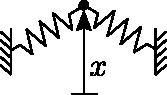
\includegraphics[width=0.11\textheight,valign=t]{Bilder/01EinMassenSchwinger.pdf}}\hspace{15mm}
	\subfloat{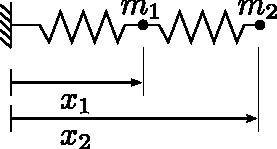
\includegraphics[width=0.155\textheight,valign=t]{Bilder/01ZweiMassenSchwinger.pdf}}\hspace{15mm}
	\subfloat{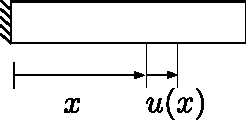
\includegraphics[width=0.14\textheight,valign=t]{Bilder/01DehnSchwinger.pdf}}
% 	\subfloat{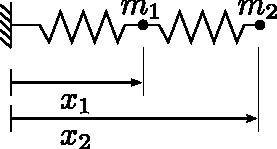
\includegraphics[width=0.3\textwidth]{Bilder/01ZweiMassenSchwinger.pdf}
	\caption{Schwingungen eines 1-, 2- und $\infty-$Freiheitsgrad-Systems}
\end{figure}
Die Schwingungsformen des betrachteten K�rpers treten in Abh�ngigkeit von der Frequenz der Anregung auf. Am Beispiel eines 4-Freiheitsgradschwingers k�nnen vier verschiedene Schwingungsformen dargestellt werden (Abb. \ref{Abb:Schwingformen4DoF}), bei denen sich die einzelnen Freiheitsgrade wechselweise in Gleich- oder Gegenphase bewegen. 
\begin{figure}[h]
	\centering
	\subfloat[Erste Schwingungsform]{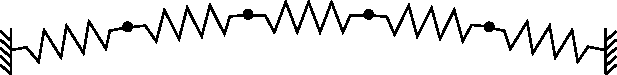
\includegraphics[width=0.3\textheight]{Bilder/01Schwingformen01.pdf}}\hfill
	\subfloat[Zweite Schwingungsform]{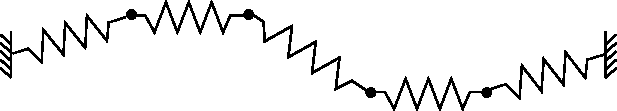
\includegraphics[width=0.3\textheight]{Bilder/01Schwingformen02.pdf}}\\[5mm]
	\subfloat[Dritte Schwingungsform]{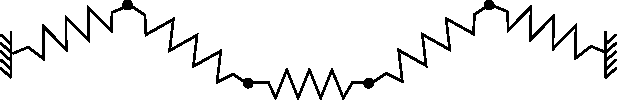
\includegraphics[width=0.3\textheight]{Bilder/01Schwingformen03.pdf}}\hfill
	\subfloat[Vierte Schwingungsform]{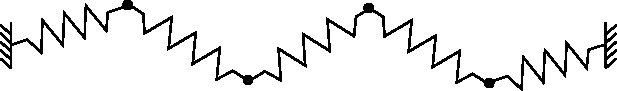
\includegraphics[width=0.3\textheight]{Bilder/01Schwingformen04.pdf}}
	% 	\subfloat{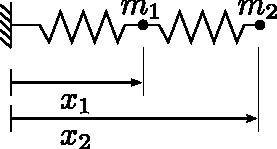
\includegraphics[width=0.3\textwidth]{Bilder/01ZweiMassenSchwinger.pdf}
	\caption{Schwingungsformen eines $4-$Freiheitsgrad-Systems}
	\label{Abb:Schwingformen4DoF}
\end{figure}
%\paragraph{Klassifikation nach Aufbau der Bewegungsgleichung}
%\begin{itemize}
%	\item Linear: geralisierte Koordinaten und Zeitableitungen treten nur linear in der Bewegungsgleichung auf. Allgemeine Form: 
%	\begin{align}
%		&M \ddot q + P \dot q + Q q = f(t)& &q \in \mathbb{R}^n&
%	\end{align}
%	\item Nichtlinear: geralisierte Koordinaten und Zeitableitungen treten nichtlinear in der Bewegungsgleichung auf. Die allgemeine Form lautet:
%	\begin{align}
%	&M (q,\dot q) \ddot q =F(t,q,\dot q)& &q \in \mathbb{R}^n&
%	\end{align}
%\end{itemize}
\section{Entstehungmechanismen von Schwingungen}
\subsection{Freie Schwingungen} 
Gitarrensaiten, Stimmgabeln oder Beispiele aus der Technik werden durch Mechanismen einmalig angesto�en oder angezupft und dann sich selbst �berlassen. Die Bewegung, die sich dann einstellt, nennt sich freie Schwingung, da die Ursache nur einmalig am Anfang der Beobachtung steht und dann instantan verschwindet. Die Schwingungsfrequenzen sind Eigenfrequenzen des Schwingungssystems. 
\subsection{Erzwungene Schwingung}
Ein Fahrzeug, welches sich �ber eine unebene Fahrbahn bewegt, wird durch �u�ere Kr�fte und/oder Momente permanent zu Schwingungen angeregt. Die Frequenz dieser Bewegung und vergleichbarer Beispiele ist im station�ren Schwingungszustand die Frequenz $\Omega$, die durch die �u�ere Anregung gegeben ist.
\subsection{Selbsterregte Schwingung}
Schwingungen wie beim Bremsenquietschen, Streichinstrumenten oder in einer mechanischen Uhr sind selbsterregt, da sich im Gesamtsystem eine Energiequelle und -Senke findet. Die Schwingungsfrequenz entspricht in vielen F�llen einer Eigenfrequenz, wobei sich hier aufgrund der komplexen Schwingungsursache und m�glicherweise dominanter Nichtlinearit�ten Abweichungen ergeben k�nnen.
\subsection{Parametererregte Schwingung}
Bei Schwingungen, die durch periodisch zeitver�nderliche Parameter im System (Steifigkeiten, Abst�nde, ...) entstehen, spricht man von parametererregten Schwingungen. Ein Beispiel aus der Technik ist im W�lzkontakt von Getrieben zu finden, wo die wechselnde Anzahl von Verzahnungseingriffen zu einer zeitver�nderlichen Steifigkeit f�hrt; ein weiteres Beispiel ist die periodische Schwerpunktverlagerung eines Kindes auf einer Schaukel, was die gew�nschte Bewegung erzeugt. Daher handelt es sich bei den Schwingungsfrequenzen auch um Teile oder Vielfache der Parameterfrequenz.
% !TeX spellcheck = de_DE
\chapter{Freie Schwingungen}
In diesem Abschnitt werden freie Schwingungen von mechanischen 1-Freiheitsgrad-Systemen untersucht, die nach einer Anfangsauslenkung sich selbst �berlassen werden. Es sollen nur statische Kr�fte auf die betrachteten Systeme wirken. 
\section{Freie unged�mpfte Schwingungen}\label{kap:UngedaempftEMS}
Ausgangspunkt f�r die freien unged�mpften Schwingungen ist ein 1-Massen-Schwinger mit nichtlinearer Federkraft $f(x)$. 
\begin{figure}[h]
	\centering
	\subfloat{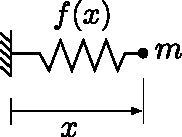
\includegraphics[width=0.11\textheight,valign=t]{Bilder/02EinMassenSchwinger.pdf}}\hspace{15mm}
	\subfloat{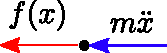
\includegraphics[width=0.11\textheight,valign=t]{Bilder/02EinMassenSchwingerdAlembert.pdf}}
	\caption{Einmassenschwinger mit nichtlinearer Kennlinie sowie dessen Kr�ftefreischnitt nach d'Alembert, wobei $m\ddot x$ die d'Alembert'sche Tr�gheitskraft ist und $f(x)$ die Federkraft.}
\end{figure}\\
Die Bilanz der Kr�fte liefert: 
\begin{align}
	m \ddot x + f(x) = 0
\label{eq:21}
\end{align}\\
Eine solche Differentialgleichung (DGL) ist aufgrund des nichtlinearen Zusammenhangs $f(x)$ im Allgemeinen nicht analytisch l�sbar. Wenn dennoch eine Analyse durchgef�hrt werden soll, dann kann die Gleichung \ref{eq:21} als n�chstes linearisiert werden (Mechanik 2.1). Nach dieser Vereinfachung beschreibt die Gleichung nur noch die Dynamik kleiner St�rungen $\Delta x$ um eine Ruhelage $x_0$, was aber in vielen F�llen in der Praxis ausreichend ist. Die Linearisierung wird nach dem Satz von Taylor (Mathematik 2.1) durchgef�hrt. 
\begin{figure}[h]
	\centering
	\begin{tikzpicture}
	\begin{axis}[
	domain=-0.5:2,
	xmin=-1,xmax=2,ymin=-3,ymax=3, 
	samples=100,
	grid=both,
	x label style={at={(axis description cs:0.5,-0.1)},anchor=north},
	y label style={at={(axis description cs:-0.1,.5)},rotate=0,anchor=south},
	xlabel={$x$},
	ylabel={$f(x)$}, 
	xtick={0,1}, 
	ytick={0}, 
	xticklabels={0,$x_0$}]
	\addplot[blue, ultra thick] {(x-1)+(x-1)*(x-1)*(x-1)};
	\addplot[black, dashed, ultra thick] {(x-1)};
	\legend{$f(x)$, Linearisierung um $x_0$}
	\end{axis}
	\end{tikzpicture}
	\caption{Nichtlineare Federkennlinie}
\end{figure} \\\newpage
\begin{theo}[Taylorreihen-Entwicklung]{theo:taylor}
Sei $f(x)$ eine $n-$mal stetig differenzierbare Funktion und $x_0$ ein Entwicklungspunkt. Dann ist die Taylorreihenentwicklung definiert als 
\[f(x) = \sum_{k=0}^{n}\frac{\textrm{d}^k f(x_0)}{\textrm{d} x^k} \frac{\left(x-x_0\right)^k}{k !} = f(x_0) + f'(x_0) (x-x_0) + f''(x_0) \frac{(x-x_0)^2}{2} + ...\]
Die Reihendarstellung konvergiert f�r $n\rightarrow\infty$ mit $f(x)$, falls $f(x)$ $\infty-$mal stetig differenzierbar ist.
\end{theo}
\begin{lem}[Linearisierung um eine Ruhelage]{lem:linearisierung}
	Zur Linearisierung einer DGL um eine Ruhelage werden folgende Schritte befolgt: 
	\begin{itemize}
		\item \textbf{Berechnung der Ruhelage:} setze $x=x_0=$konst., dann ist $\dot x=0$, $\ddot x=0$. Einsetzen in die DGL liefert eine algebraische Gleichung zur Bestimmung der Ruhelage(n): 
		\[f(x_0)=0\]
		\item \textbf{Definition der St�rung} $\Delta x$ um die Ruhelage $x_0$: $x=x_0+\Delta x$. Einsetzen in die DGL ergibt 
		\[m\Delta \ddot x + f(x_0 + \Delta x)=0\]
		\item \textbf{Linearisierung:} Taylorreihen-Entwicklung der nichtlinearen Funktion $f(x_0+\Delta x)$ in der St�rung $\Delta x$ bis zur 1. Ordnung: 
		\[f(x_0 + \Delta x)\approx f(x_0) + f'(x_0)\cdot \Delta x\]
		\item \textbf{Einsetzen und vereinfachen:}
		\[m\Delta \ddot x + f(x_0) + f'(x_0)\cdot \Delta x = 0\]
		Der Term $f(x_0)$ verschwindet, da aus ihm die Ruhelage berechnet wurde. Es bleibt die homogene lineare DGL mit konstanten Koeffizienten f�r die Beschreibung der kleinen St�rung um die Ruhelage
		\[m\Delta \ddot x + f'(x_0)\cdot \Delta x = 0\]
	\end{itemize}
\end{lem}
\begin{beispiel}[Nichtlineare Federkennlinie]{beispiel:linearisierung}
Eine Federkennlinie kann beschrieben werden durch den Kraft-Weg-Zusammenhang $f(x) = \sin(x) + a_1 x + a_3 x^3$. Die DGL des 1-Massen-Schwingers lautet somit: 
\begin{align*}
m \ddot x + \sin(x) + a_1 x + a_3 x^3 = 0
\end{align*}
Die Ruhelage berechnet sich aus der Gleichung
\begin{align*}
\sin(x_0) + a_1 x_0 + a_3 x_0^3 = 0
\end{align*}
zu $x_0=0$. Die DGL in der St�rung um $x_0$ ist also 
\begin{align*}
0 = &m(\ddot x_0+\Delta \ddot x) + \sin(x_0) + a_1 (x_0+x) + a_3 (x_0+x)^3 \\
= &m\Delta \ddot x + \sin(x_0+x) + a_1 (x_0+x) + a_3 (x_0+x)^3 \\
= &m\Delta \ddot x + \sin(x_0) + a_1 x_0 + a_3 (x_0)^3 + \left(\cos(x_0)+a_1 +3 x_0^2\right)\Delta x\\
\approx &m\Delta \ddot x + \left(1+a_1\right)\Delta x
\end{align*}
Hier ist $f'(x_0)=1+a_1=c$ die lokale Steifigkeit in der N�he der Ruhelage. Alternativ wird die DGL 
\begin{align*}
\Delta \ddot x + \omega_0^2 \Delta x=0, 
% \label{eq:27}
\end{align*}
wobei $\omega_0^2 = \frac{f'(x_0)}{m}=\frac{c}{m}$ das Quadrat der unged�mpften Eigenkreisfrequenz ist. 
\end{beispiel}
Die Koeffizienten der DGL \ref{eq:21} sind konstant, weshalb als L�sungsansatz f�r die homogene L�sung der Exponentialansatz verwendet werden kann: 
\begin{theo}[Lineare homogene DGL mit konstanten Koeffizienten]{theo:konstKoeff}
	Eine lineare homogene DGL mit konstanten Koeffizienten 
	\begin{align}
	\sum_{k=0}^{n} a_k \frac{\textrm{d}^k x(t)}{\textrm d t^k} = a_n \frac{\textrm{d}^n x(t)}{\textrm d t^n}+...+a_1 \frac{\textrm{d} x(t)}{\textrm d t} + a_0 x(t)=0\nonumber
	\end{align}
	wird mithilfe des Exponentialansatzes 
	\begin{align}
	x(t)=C e^{\lambda t} \nonumber
	\end{align}
	gel�st. Der Ansatz eingesetzt in die DGL liefert das Eigenwertproblem 
	\begin{align}
	\sum_{k=0}^{n} a_k C \lambda^k e^{\lambda t} 
	= \left(\sum_{k=0}^{n} a_k \lambda^k\right)C e^{\lambda t} =0.\nonumber 
	\end{align}
	Wegen $C\neq 0$ folgt das charakteristische Polynom
	\begin{align}
	\sum_{k=0}^{n} a_k \lambda^k = a_n \lambda^n + ... +a_1 \lambda +a_0 =0\nonumber 
	\end{align}
	woraus die Eigenwerte $\lambda_{1,2,...,n}$ bestimmt werden. Die L�sungsanteile 
	\begin{align}
	x_k(t) = C_k e^{\lambda_k t}\nonumber 
	\end{align}
	werden \emph{Fundamentall�sungen} genannt; die Gesamtl�sung setzt sich aus ihnen zusammen: 
	\begin{align}
	x(t) = \sum_{k=0}^{n} C_k x_k(t) = C_n e^{\lambda_n t} +...+ C_2 e^{\lambda_2 t} + C_1 e^{\lambda_1 t}. \nonumber 
	\end{align}
	Die Integrationskonstanten $C_k$ m�ssen durch geeignete Anfangsbedingungen bestimmt werden. 
\end{theo}
Nach dem beschriebenen Vorgehen in (Mathematik 2.2) und $f'(x_0)=:c$ lautet die DGL der St�rung zur Gl. \ref{eq:21}
\begin{align}
&m\Delta \ddot x + c \Delta x = 0 &&\textrm{bzw.}&&\Delta \ddot x + \underbrace{\frac{c}{m}}_{:=\omega_0^2} \Delta x = 0 &\label{eq:27}
\end{align}
Der L�sungsansatz und dessen Ableitungen sind 
\begin{align}
& \Delta x =A e^{\lambda t}, &
& \Delta \dot x =\lambda A e^{\lambda t}, &&
&\Delta \ddot x =\lambda^2 A e^{\lambda t} &&
\end{align}
Dies eingesetzt in Gl. \ref{eq:21} liefert 
\begin{align}
& (\lambda^2 +\omega_0^2) A e^{\lambda t}=0, &
& \textrm{woraus folgt} &
& \lambda_{1,2} =\pm i \omega_0.&
\end{align}
Somit gibt es zwei komplexe Fundamentall�sungen 
\begin{align}
& x_1(t) = A_1 e^{i \omega_0 t}, &
& x_2(t) = A_2 e^{-i \omega_0 t} &
\end{align}
Die Gesamtl�sung ergibt sich unter Beschr�nkung auf rein reelle L�sungen zu 
\begin{align}
	x(t) &= Re\{x_1(t) + x_2(t)\}\\
	& = Re\{A_1 e^{i \omega_0 t} + A_2 e^{-i \omega_0 t}\}\nonumber \\
	& = Re\{A_1 +A_2 \} \cos(\omega_0 t) + Re\{i A_1 -i A_2 \} \sin(\omega_0 t)\nonumber \\
	& = C_1 \cos(\omega_0 t) + C_2 \sin(\omega_0 t)\nonumber 
\end{align}
Hierbei wurde zur Transformation die Euler-Formel verwendet: 
\begin{theo}[Euler-Formel]{theo:Euler}
	Es gilt der Zusammenhang 
	\begin{align}
	e^{i\varphi}=\cos(\varphi)+i\sin(\varphi)\nonumber 
	\end{align}
\end{theo}
Die Kreisfrequenz $\omega_0$ wurde bereits durch Masse und Steifigkeit festgelegt und h�ngt somit nur von Systemparametern ab. Sie ist dem System \emph{eigen} und hei�t deshalb \emph{Eigenkreisfrequenz}.\\
Als Parameter bleiben die Integrationskonstanten $C$ und $S$, die durch die Anfangsbedingungen (Anfangslage und, Anfangsgeschwindigkeit) festgelegt werden: 
\begin{align}
	x(t=0) &=  C_1 \cos(0) + C_2 \sin(0)  = C_1 \overset{!}{=}x_0\\
	\dot x(t=0) &= -C_1 \omega_0 \sin(0) + C_2 \omega_0 \cos(0)  = C_2 \omega_0 \overset{!}{=}v_0
\end{align}
Als Gesamtl�sung ergibt sich so 
\begin{align}
x(t) &=  x_0 \cos(\omega_0 t) + \frac{v_0}{\omega_0} \sin(\omega_0 t)  
\end{align}
Die Schwingungsdauer der Bewegung ist $T=\frac{2\pi}{\omega_0}$.
\begin{beispiel}[Mathematisches Pendel]{beispiel:mathPendel}
Ein mathematisches Pendel besteht aus einem masselosen Stab der L�nge $\ell$, der einseitig an einem Gelenk befestigt ist. An seinem freien Ende befindet sich ein Gewicht mit Punktmasse $m$. Das System ist der Schwerkraft unterworfen (Gravitationskonstante $g$). Die Auslenkung wird durch den Verdrehwinkel $\varphi$ beschrieben. \\[2mm]
\hspace*{3cm}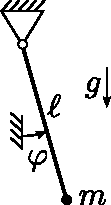
\includegraphics[width=0.12\textwidth]{Bilder/02MathematischesPendel.pdf} \\[2mm]
Die Bewegungsgleichung folgt aus der Momentenbilanz um das Gelenk und lautet
\begin{align*}
&m \ell^2 \ddot \varphi + m g \ell \sin(\varphi) = 0& 
&\textrm{bzw.}&
&\ddot \varphi + \frac{g}{\ell}\sin(\varphi) = 0& 
\end{align*}
Diese DGL ist zun�chst nichtlinear. Bei der Bestimmung der Ruhelagen finden sich zwei L�sungen: 
\begin{align*}
	&\ddot \varphi=0&& \rightarrow&
	&\frac{g}{\ell}\sin(\varphi) = 0&
\end{align*}
also 
\begin{align*}
&\varphi_{0,1} = 0, &&\varphi_{0,2} = \pi.&\\
&\textrm{(H�ngelage)} &&\textrm{(�berkopflage)} &
\end{align*}
\paragraph{Linearisierung um die H�ngelage:} Die Linearisierung der Nichtlinearit�t um die Ruhelage $\varphi_{0,1}=0$ lautet 
\begin{align*}
	\frac{g}{\ell}\sin(\varphi) \approx \frac{g}{\ell}\sin(\varphi_{0,1}) + \frac{g}{\ell}\cos(\varphi_{0,1})\cdot (\varphi - \varphi_{0,1}) = \frac{g}{\ell}(\varphi - \varphi_{0,1}) = \frac{g}{\ell}\Delta \varphi
\end{align*}
wobei $\Delta\varphi$ die St�rung um die Ruhelage ist. Au�erdem ist 
\begin{align*}
	\Delta \ddot \varphi = \ddot \varphi -0 = \ddot \varphi
\end{align*}
Somit lautet die linearisierte DGL
\begin{align*}
&\Delta \ddot \varphi + \frac{g}{\ell}\Delta \varphi = 0&
&\textrm{oder}&
&\Delta \ddot \varphi + \omega_0^2\Delta \varphi = 0&
\end{align*}
mit $\omega_0^2 = \frac{g}{\ell}$. Die DGL hat nun exakt die Form der Gl. (2.2), weshalb die L�sung direkt angegeben werden kann: 
\begin{align*}
\varphi(t) &=  \varphi_0 \cos(\omega_0 t) + \frac{\dot\varphi_0}{\omega_0} \sin(\omega_0 t)  
\end{align*}
Interpretation: F�r kleine Anfangswinkel $\varphi_0$ und kleine Anfangsgeschwindigkeiten $\dot \varphi_0$ bleibt die L�sung $\varphi(t)$ f�r alle Zeiten klein. Die Linearisierung beschriebt das Systemverhalten gut. 
\paragraph{Linearisierung um die �berkopflage:} Die Linearisierung der Nichtlinearit�t um die Ruhelage $\varphi_{0,2}=\pi$ lautet 
\begin{align*}
\frac{g}{\ell}\sin(\varphi) \approx \frac{g}{\ell}\sin(\varphi_{0,2}) + \frac{g}{\ell}\cos(\varphi_{0,2})\cdot (\varphi - \varphi_{0,2}) = -\frac{g}{\ell}(\varphi - \varphi_{0,2}) = -\frac{g}{\ell}\Delta \varphi
\end{align*}
Somit lautet die linearisierte DGL
\begin{align*}
&\Delta \ddot \varphi - \frac{g}{\ell}\Delta \varphi = 0&
\end{align*}
Dies entspricht wegen des negativen Vorzeichens nicht der Form der Gl. (2.2), kann aber trotzdem mithilfe eines Exponentialansatzes $\Delta \varphi = C e^{\lambda t}$ gel�st werden. Dieser ergibt nach Einsetzen die Eigenwerte 
\begin{align*}
	\lambda_{1,2}=\pm \sqrt{\frac{g}{\ell}}=\pm \delta
\end{align*}
also zwei reelle Eigenwerte. Die zwei Fundamentall�sungen 
\begin{align*}
&\Delta \varphi_1 =C_1 e^{\delta t}&&\Delta \varphi_2 = C_2 e^{-\delta t}&
\end{align*}
ergeben die Gesamtl�sung 
\begin{align*}
\Delta \varphi = C_1 e^{\delta t}+C_2 e^{-\delta t}
\end{align*}
Anpassen an die Anfangslage $\varphi(t=0)$ und Anfangsgeschwindigkeit $\dot \varphi(t=0)$ liefert schlie�lich die Gesamtl�sung 
\begin{align*}
\Delta \varphi = \frac{\varphi_0+\frac{\dot \varphi_0}{\delta}}{2} e^{\delta t}+ \frac{\varphi_0-\frac{\dot \varphi_0}{\delta}}{2}  e^{-\delta t}
\end{align*}
Interpretation: Nach einer St�rung in der Auslenkung und/oder Geschwindigkeit zum Zeitpunkt $t=0$ klingt die L�sung in der N�he der �berkopflage exponentiell auf. Sie ist im Gegensatz zur H�ngelage nicht schwingungsf�hig. Die linearisierte L�sung beschreibt das qualitative Verhalten korrekt, ist aber quantitativ h�chstens f�r eine sehr kurze Zeitdauer richtig. 
\end{beispiel}

\paragraph{Fazit.} Eine Linearisierung um unterschiedliche Ruhelagen liefert im Allgemeinen verschiedene Bewegungsgleichungen, die verschiedene Eigenschaften haben k�nnen. 
\section{Freie ged�mpfte Schwingungen}
Im ged�mpften Einmassenschwinger wird zus�tzlich parallel zur Federkraft ein D�mpfer geschaltet, sodass sich das System um die D�mpferkraft erweitert: 
\begin{figure}[h]
	\centering
	\subfloat{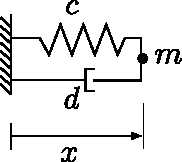
\includegraphics[width=0.11\textheight,valign=c]{Bilder/02EinMassenSchwingerDamped.pdf}}\hspace{15mm}
	\subfloat{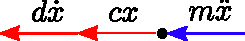
\includegraphics[width=0.15\textheight,valign=c]{Bilder/02EinMassenSchwingerDampeddAlembert.pdf}}
	\caption{Linearer ged�mpfter Einmassenschwinger sowie dessen Kr�ftefreischnitt nach d'Alembert, wobei $m\ddot x$ die d'Alembert'sche Tr�gheitskraft ist, $c x$ die Federkraft und $d\dot x$ die D�mpferkraft.}
\end{figure}\\
Der unged�mpfte Einmassenschwinger (Kapitel \ref{kap:UngedaempftEMS}) stellt somit den Sonderfall $d=0$ dar. 
Die Kr�ftebilanz liefert
\begin{align}
	&m\ddot x + d\dot x + c x= 0 &&\textrm{bzw.}&\label{eq:GedEMS}\\
	&\ddot x + \frac{d}{m}\dot x + \frac{c}{m} x= 0 &\nonumber 
\end{align}
\begin{lem}[Parameter des ged�mpften Einmassenschwingers]{lem:ged1ms}
	Zur einheitlichen Beschreibung werden die folgenden Parameter eingef�hrt: 
	\begin{itemize}
		\item Unged�mpfte Eigenkreisfrequenz: $\omega_0 = \sqrt{\frac{c}{m}}$
		\item Exponentielle Abklingrate: $\delta = \frac{d}{2m}$
		\item Lehr'sches D�mpfungsma�: $D = \frac{d}{2 m \omega_0}$
		\item Ged�mpfte Eigenkreisfrequenz $\omega_d = \omega_0 \sqrt{1-D^2}$
		\item Schwingungsdauer $T = 2\pi/\omega_d$
	\end{itemize}
\end{lem}
Die vereinfachte Gleichung des homogenen ged�mpften Einmassenschwingers lautet nach (Mechanik 2.2): 
\begin{align}
\ddot x + 2D \omega_0 \dot x +\omega_0^2 x =0\label{eq:GedEMSD}
\end{align}
\begin{beispiel}[Nichlinearer Einmassenschwinger mit D�mpfung]{beispiel:EMSDamp}
Die DGL lautet in diesem Beispiel
\begin{align}
(J + m R^2 )\ddot x + d\dot x \cos(x) + c_0 x + c_3 x^3 = 0 \nonumber
\end{align}
wobei alle Koeffizienten positive Werte haben sollen. Das Ziel ist, auf die Form (2.11) zu kommen. Dazu werden zun�chst die Ruhelagen bestimmt. Mit $x=x_0$, $\dot x=0$, $\ddot x=0$ folgt 
\begin{align}
&c_0 x_0 + c_3 x_0^3 = 0,&&\textrm{ weshalb}&&x_{0,1}=0,&&x_{0,2/3}=\pm\sqrt{-c_0/c_3}&\nonumber
\end{align}
Mit $c_0>0$, $c_3>0$ ist nur die Ruhelagen $x_{0,1}$ physikalisch sinnvoll. Also wird um diese Ruhelage linearisiert. Es ist 
\begin{align}
f(x,\dot x) &= d\dot x \cos(x) + c_0 x + c_3 x^3\nonumber \\
f(x_{0,1}+\Delta x,\Delta \dot x) &= d \Delta \dot x \cos(x_{0,1}+\Delta x) + c_0 (x_{0,1}+\Delta x) + c_3 (x_{0,1}+\Delta x)^3\nonumber \\
&= d \Delta \dot x \cos(\Delta x) + c_0 \Delta x + c_3 \Delta x^3\nonumber \\
&\approx d \Delta \dot x \cdot (\cos(0)-\cancel{\sin(0)\cdot \Delta x})+ c_0 \Delta x + \cancel{c_3 \Delta x^3}\nonumber \\
&= d \Delta \dot x +c_0 \Delta x\nonumber
\end{align}
Also folgt die linearisierte DGL 
\begin{align}
(J + m R^2 )\Delta \ddot x + d\Delta \dot x + c_0 \Delta x \nonumber 
\end{align}
Sie l�sst sich auf die Form der Gl. (2.11) bringen, wenn die Koeffizienten 
\begin{align}
& \omega_0^2 = \frac{c_0}{J + m R^2 } && D = \frac{d}{2}\sqrt{\frac{1}{c_0 (J+mR^2)}}&\nonumber
\end{align}
gew�hlt werden. \\
\end{beispiel}
Die Fundamentall�sung der Gl. \ref{eq:GedEMSD} ist mit $\lambda_{1,2}=-D\omega_0\pm\omega_0\sqrt{D^2-1}$
\begin{align}
x = C_1 e^{\lambda_1 t} + C_2 e^{\lambda_2 t}
\end{align}
Welchen qualitativen Verlauf die L�sung annimmt, h�ngt ma�geblich mit der Gr��e des Lehr'schen D�mpfungsma�es $D$ zusammen: 
\paragraph{Fall 1: starke D�mpfung.} Bei $D>1$ gilt 
\begin{align}
&	\lambda_1 = -D\omega_0+\omega_0\sqrt{D^2-1}<0&& \lambda_2 = -D\omega_0-\omega_0\sqrt{D^2-1}<0
\end{align}
Die L�sung $x = C_1 x_1 + C_2 x_2$ setzt sich also aus zwei Anteilen zusammen, deren Verlauf wegen der $\lambda_i<0$ immer expontiell abklingt. Da hiermit Schwingungen ausgeschlossen sind, wird die Bewegung auch \emph{Kriechbewegung} genannt. 
\paragraph{Fall 2: aperiodischer Grenzfall.} Bei $D=1$ fallen die zwei Eigenwerte zusammen: 
\begin{align}
&	\lambda_1 = \lambda_2 = -D\omega_0=-\delta &
\end{align}
Aufgrund des doppelten Eigenwerts ist die L�sung $x=C_1 e^{\lambda t}+C_2 t e^{\lambda t}$.
\paragraph{Fall 3: schwache D�mpfung.} Bei $0<D<1$ ist 
\begin{align}
&	D^2-1<0,& &\textrm{also}&& \omega_0\sqrt{D^2-1}=i\omega_0\sqrt{1-D^2}=i\omega_d& 
\end{align}
mit $i$ der komplexen Zahl. Die (komplexe) Fundamentall�sung kann hier transformiert werden in reellwertige Funktionen: 
\begin{align}
	x &= \tilde{C}_1 e^{-\delta t+i \omega_d t} + \tilde{C}_2 e^{-\delta t-i \omega_d t}\\
	 &= e^{-\delta t}\left(\tilde{C}_1 e^{i \omega_d t} + \tilde{C}_2 e^{-i \omega_d t}\right)\nonumber\\
	 &= e^{-\delta t}\left(C_1\cos(\omega_d t) + C_2\sin(\omega_d t)\right)\nonumber
\end{align}
Es handelt sich bei der Bewegung um eine ged�mpfte Schwingung mit Kreisfrequenz $\omega_d<\omega_0$, deren Amplitude mit zunehmender Zeit exponentiell abklingt. 
\begin{figure}[h]
	\centering
	\begin{tikzpicture}
	\begin{axis}[
	domain=0:10,
	xmin=0,xmax=10,ymin=-1.2,ymax=1.2, 
	samples=1000,
	grid=both,
	x label style={at={(axis description cs:0.5,-0.1)},anchor=north},
	y label style={at={(axis description cs:-0.1,.5)},rotate=0,anchor=south},
	xlabel={$t$},
	ylabel={$x(t)$}]
	\addplot[blue, ultra thick] {exp(-x/2)*cos(2*pi*deg(x))};
	\addplot[black, dashed] {-exp(-x/2)};
	\addplot[black, dashed] { exp(-x/2)};
	\end{axis}
	\end{tikzpicture}
	\caption{Verlauf einer ged�mpften Schwingung.}
\end{figure}\\
Es l�sst sich zeigen, dass das Ma� der Amplitudenreduktion gegeben ist durch 
\begin{align}
	\frac{x(t)}{x(t+T_d)} = e^{\delta T_d}
\end{align} 
Daraus folgt direkt das \emph{logarithmische Dekrement}: 
\begin{align}
\Lambda := \ln\left(\frac{x(t)}{x(t+T_d)}\right) = \delta T_d = D \omega_0 T_d
\end{align} 
Mit bekanntem $\omega_0$, gemessenen $T_d$ und $\Lambda$ l�sst sich so aus einer Messung das Lehr'sche D�mpfungsma� bestimmen. 
\section*{Aufgaben zu Kapitel 2}
\paragraph{2.1} Welche Unterschiede gibt es zwischen unged�mpften und ged�mpften Schwingungen?
\paragraph{2.2} Mit welchen standardisierten Parametern (Konstanten) l�sst sich ein lineares mechanisches Schwingungssystem mit einem Freiheigsgrad beschreiben? Welche Bedeutung haben sie?
\paragraph{2.3} Welche Eigenschaften muss eine DGL haben, damit sie mit einem Exponentialansatz gel�st werden kann?
\paragraph{2.4} Linearisieren Sie die folgenden Ausdr�cke in der Variable $x$ um den Entwicklungspunkt $x=0$: 
\begin{align}
	& y = x^2+\sin(x) + \frac{e^x}{1+x} && y = \frac{a x +b}{c x + d}&
\end{align}
\paragraph{2.5} Bestimmen Sie die Ruhelage(n) der folgenden DGLn: 
\begin{align}
	& \ddot x + c_1 x - c_3 x^3=0 && \ddot x + d\dot x + c_1 \sin(k x)=0&\\
	& \ddot x + (d_1 + d_2 )\dot x + c_1 x + c_2 x^2=0&
\end{align}
Linearisieren Sie die DGL anschlie�end f�r kleine St�rungen $\Delta x = x-x_0$ um jede berechnete Ruhelage $x_0$! 
\paragraph{2.6} Bestimmen Sie f�r die DGL
\begin{align}
	(m+R^2 J) \ddot x + m e \Omega^2\dot x + c_0 x=0
\end{align}
die Ersatzparameter $\omega_0$, $\omega_d$, $D$, $\delta$, und geben Sie die L�sung der DGL in allgemeiner Form an! Passen Sie die Integrationskonstanten an die Anfangsbedingungen $x (t=0)=0$ und $\dot{x}(t=0) = v_0$ an. 
% !TeX spellcheck = de_DE
\chapter{Erzwungene Schwingungen}
In diesem Kapitel wird die Situation betrachtet, dass der Einmassenschwinger harmonisch wirkenden Kr�ften oder vorgegebenen Bewegungen ausgesetzt ist:
\begin{figure}[h]
	\centering
	\subfloat[Kraft]{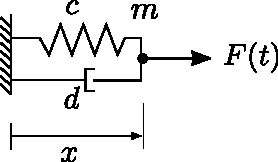
\includegraphics[height=0.13\textwidth]{Bilder/03EinMassenSchwinger}\label{abb:ErzKraft}}\hfill
	\subfloat[Fu�punkt (Maxwell)]{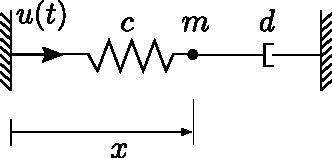
\includegraphics[height=0.13\textwidth]{Bilder/03EinMassenSchwingeruMaxwell}\label{abb:ErzMaxwell}}\hfill
	\subfloat[Fu�punkt (Voigt)]{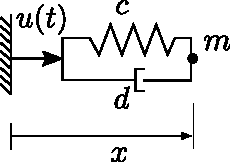
\includegraphics[height=0.13\textwidth]{Bilder/03EinMassenSchwingeru}\label{abb:ErzVoigt}}\hfill
	\subfloat[Unwucht]{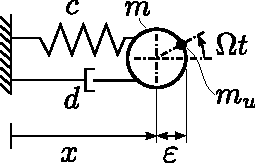
\includegraphics[height=0.13\textwidth]{Bilder/03EinMassenSchwingerExz}\label{abb:ErzUnwucht}}
	\caption{Einmassenschwinger mit Anregung durch �u�ere Kraft, durch Fu�punkt- und durch und durch Unwuchterregung.}
	\label{abb:Anregungen}
\end{figure}\\
Dies �ndert die Sachlage insofern, als dass die Bewegung $x(t)$ aus zwei Anteilen besteht: einer \emph{homogenen} und einer \emph{partikul�ren} Bewegung bzw. L�sung der DGL. 
\begin{align}
	x(t) = x_h(t) + x_p(t)
\end{align}
\begin{figure}[h]
	\centering
	\subfloat{
		\begin{tikzpicture}
		\begin{axis}[
		scale=0.55,
		domain=0:10,
		xmin=0,xmax=10,ymin=-2,ymax=2, 
		samples=1000,
		grid=both,
		x label style={at={(axis description cs:0.5,-0.1)},anchor=north},
		y label style={at={(axis description cs:-0.1,.5)},rotate=0,anchor=south},
		xlabel={$t$},
		ylabel={$x_h(t)$}]
		\addplot[blue, ultra thick] {exp(-x/2)*cos(2*pi*deg(x))};
		\addplot[black, dashed] {-exp(-x/2)};
		\addplot[black, dashed] { exp(-x/2)};
		\end{axis}
		\end{tikzpicture}}
	\subfloat{
		\begin{tikzpicture}
		\begin{axis}[
		scale=0.55,
		domain=0:10,
		xmin=0,xmax=10,ymin=-2,ymax=2, 
		samples=1000,
		grid=both,
		x label style={at={(axis description cs:0.5,-0.1)},anchor=north},
		y label style={at={(axis description cs:-0.1,.5)},rotate=0,anchor=south},
		xlabel={$t$},
		ylabel={$x_p(t)$}]
		\addplot[red, ultra thick,dashed] {sin(2*pi/3.2*deg(x))};
		\end{axis}
		\end{tikzpicture}}
	\subfloat{
		\begin{tikzpicture}
		\begin{axis}[
		scale=0.55,
		domain=0:10,
		xmin=0,xmax=10,ymin=-2,ymax=2, 
		samples=1000,
		grid=both,
		x label style={at={(axis description cs:0.5,-0.1)},anchor=north},
		y label style={at={(axis description cs:-0.12,.5)},rotate=0,anchor=south},
		xlabel={$t$},
		ylabel={$x(t)=x_h(t)+x_p(t)$}]
		\addplot[red, ultra thick,dashed] {sin(2*pi/3.2*deg(x))};
		\addplot[blue, ultra thick] {exp(-x/2)*cos(2*pi*deg(x))+sin(2*pi/3.2*deg(x))};
		\end{axis}
		\end{tikzpicture}}
	\caption{Erzwungene Schwingung, die sich als Summe von $x_h(t)$ und $x_p(t)$ zusammensetzt.}
\end{figure}\\
\begin{itemize}
	\item Die homogene L�sung wurde bereits in Kapitel 2 betrachtet. Dieser Anteil, der die Bewegung und bzw. den Eigenschwingvorgang infolge von Anfangsauslenkungen wiedergibt, wird ab jetzt $x_h(t)$ genannt. 
	\item Die partikul�re L�sung, die durch die �u�ere Anregung vorgegeben wird, nennt sich $x_p(t)$. Er wird auch Zwangsschwingung genannt, da er die Reaktion des Schwingungssystems auf die �u�ere Anregung darstellt. 
\end{itemize}
Ferner wird von nun an vorausgesetzt, dass schwache D�mpfung (Fall 3) vorliegt. Damit klingen die harmonischen Schwingungen $x_h(t)$ mit zunehmender Zeit ab; nach kurzer Zeit bleibt die Zwangsschwingung �brig. 
Die hier betrachteten Erregungsarten umfassen gem�� Abb. \ref{abb:Anregungen}
\begin{itemize}
	\item Kraftanregung: der Einmassenschwinger wird durch eine periodische Kraft der Art ${F(t) = \hat F \cos(\Omega t+\alpha)}$ zur Schwingung angeregt. Hierbei handelt es sich bei $\Omega$ um die Kreisfrequenz der �u�eren Anregung. 
	\item Fu�punktanregung: der Fu�punkt des Einmassenschwingers wird durch eine periodische Bewegung der Art ${u(t) = \hat u \cos(\Omega t+\alpha)}$ verschoben. Hierbei handelt es sich bei $\Omega$ um die Kreisfrequenz der Verschiebung. 
	\item Unwuchtanregung: Als eine spezielle Art der Kraftanregung wird davon ausgegangen, dass die Masse des Einmassenschwingers aus einer Kreisscheibe besteht, worauf sich eine exzentrische sitzende Masse befindet. Durch Drehung der Scheibe mit Drehzahl $\Omega$ entsteht so die Fliehkraft, deren $x-$Komponente lautet: $F_u(t) = m_u\varepsilon \Omega^2 \cos(\Omega t+\alpha)$.
\end{itemize}
Der Einfachheit halber wird hier $\alpha=0$ gew�hlt, d.h. die Erregung $F(t)$ bzw. $u(t)$ beginnt bei $t=0$ mit maximaler Intensit�t. Dies stellt keine Einschr�nkung der Allgemeinheit dar: mit Transformation auf einen anderen Beobachtungsbeginn durch $t = \tilde{t}+\alpha/\Omega$ wird stets $\cos(\Omega t)=\cos(\Omega \tilde{t}+\alpha)$.
\section{Unged�mpfte krafterregte Schwingungen}
Die Bewegungsgleichung des unged�mpften Einmassenschwingers mit harmonischer Kraftanregung ergibt sich mit $F(t) = \hat F \cos(\Omega t)$ aus dem Prinzip von d'Alembert
\begin{align}
	m\ddot x + c x = F(t) = \hat F\cos (\Omega t) \label{eq:32}
\end{align}
\begin{figure}[h]
	\centering
	\subfloat{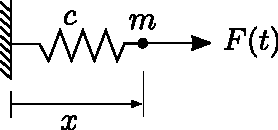
\includegraphics[height=0.11\textwidth,valign=c]{Bilder/03EinMassenSchwingerF}}\hspace{2cm}
	\subfloat{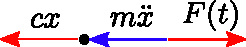
\includegraphics[height=0.04\textwidth,valign=c]{Bilder/03EinMassenSchwingerFdAlembert}}
	\caption{Einmassenschwinger ohne D�mpfung sowie die zugeh�rige Kr�ftebilanz nach dem Prinzip von d'Alembert}
\end{figure}\\
\begin{lem}[Berechnung der L�sung mit �u�erer Anregung]{lem:Gesamtl�sung}
	Das Vorgehen zur Berechnung der Gesamtl�sung $x(t)$ eines durch $y(t)$ zwangserregten Systems 
	\begin{align*}
		\ddot x(t) +2D\omega_0 \dot x(t) +\omega_0^2 x(t) = y(t)
	\end{align*}
	ist wie folgt:
	\begin{enumerate}
		\item Berechnung der homogenen L�sung gem�� Kapitel 2. Setze hierzu zun�chst die Anregung $y(t)$ zu Null, um das homogene System 
		\begin{align*}
		\ddot x(t) +2D\omega_0\dot x(t) +\omega_0^2 x(t) = 0
		\end{align*}
		zu l�sen. Die L�sung lautet $x_h(t) = e^{-\delta t}\left(C_1\cos(\omega_d t) + C_2\sin(\omega_d t)\right)$. Die Integrationskonstanten der einzelnen Fundamentall�sungen werden noch nicht an die Anfangsbedingungen angepasst. 
		\item Berechnung der partikul�ren L�sung. Hierzu wird ein \textbf{Ansatz vom Typ der rechten Seite} ben�tigt. Bei einer Anregung der Art $y(t) = y_0 + y_c \cos(\Omega t)+y_s \sin(\Omega t)$ und $i\Omega\neq \lambda$ lautet dieser Ansatz 
		\begin{align*}
		x_p(t) = X_0 + A \cos (\Omega t) + B \sin (\Omega t)
		\end{align*}
		\item Aus dem Ansatz $x_p(t)$ werden die Ableitungen $\dot x_p(t)$ und $\ddot x_p(t)$ gebildet und in die DGL eingesetzt. Nach Koeffizientenvergleich resultieren $X_0$, $A$ und $B$.
		\item Die Gesamtl�sung $x(t) = x_h(t) + x_p(t)$ beinhaltet nun noch die Integrationskonstanten $C_1$ und $C_2$, die jetzt an die Anfangsbedingungen 
		\begin{align*}
		&x(t=0) = x_0&&\dot x(t=0) = v_0&
		\end{align*}
		angepasst werden.
	\end{enumerate}
\end{lem}
Mit Einf�hrung der unged�mpften Eigenfrequenz entsteht aus Gl. \ref{eq:32} 
\begin{align}
\ddot x + \omega_0^2 x = \frac{\hat F}{m}\cos(\Omega t)\label{eq:33}
\end{align}
Die homogene L�sung lautet 
\begin{align}
x_h(t) = C_1 \cos(\omega_0 t) + C_2 \sin(\omega_0 t)
\end{align}
Die rechte Seite ist rein harmonisch, ohne Konstantanteil -- daher ist schon jetzt absehbar, dass $X_0=0$. Der Vollst�ndigkeit halber wird hier dennoch der gegebene Ansatz verwendet:  
\begin{align}
& x_p(t) = X_0 + A \cos(\Omega t) + B \sin(\Omega t)& \\
& \dot x_p(t) = -A \Omega \sin(\Omega t) + B \Omega \cos(\Omega t)& \\
& \ddot x_p(t) = -A \Omega^2\cos(\Omega t) - B \Omega^2 \sin(\Omega t)&
\end{align}
Einsetzen in Gl. \ref{eq:33} ergibt
\begin{align}
	&-A \Omega^2\cos(\Omega t) - B \Omega^2 \sin(\Omega t) +\omega_0^2(X_0 + A \cos(\Omega t) + B \sin(\Omega t)) = \frac{\hat F}{m}\cos(\Omega t)
\end{align}
Die Parameter $A$ und $B$ werden durch Koeffizientenvergleich bestimmt: 
\begin{align}
&\textrm{Konstantanteile:}& &\omega_0^2 X_0 =0& \\
&\cos(\Omega t):&& -A \Omega^2 +\omega_0^2 A = \frac{\hat F}{m}&\\
&\sin(\Omega t):&& -B \Omega^2 +\omega_0^2 B =0&
\end{align}
Die Aufl�sung des Gleichungssystems liefert 
\begin{align}
X_0=&0\\
A =&  \frac{\hat F}{m}\frac{1}{\omega_0^2-\Omega^2}\\
B =& 0
\end{align}
und mit dem dimensionslosen Frequenzverh�ltnis $\eta = \Omega/\omega_0$ ist dann 
\begin{align}
x_p(t)&=\frac{\hat F}{m}\frac{1}{\omega_0^2-\Omega^2}\cos(\Omega t) = \frac{\hat F}{m}\frac{1}{\omega_0^2}\frac{1}{1-\left(\frac{\Omega}{\omega_0}\right)^2}\cos(\Omega t)\\
&= \frac{\hat F}{c}\frac{1}{1-\eta^2}\cos(\Omega t)\\
& = \hat x \cos(\Omega t+\varphi(\eta))
\end{align}
mit der (positiven) Amplitude $\hat x = \frac{\hat F}{c}\left|\frac{1}{1-\eta^2}\right| = \frac{\hat F}{c}\frac{1}{\left|1-\eta^2\right|} $. Das Verh�ltnis 
\begin{align}
	V(\eta) = \frac{1}{\left|1-\eta^2\right|}
\end{align}
wird Vergr��erungsfunktion genannt; sie ist der ver�nderliche Teil der Amplitude $\hat x$ in Abh�ngigkeit von der Drehzahl. Ferner ist 
\begin{align}
\varphi(\eta) = \left\{\begin{array}{cc}
0,&\eta<1\\
-\pi & \eta>1
\end{array}\right.
\end{align}
die Phasenverschiebung zwischen $x_p(t)$ und der Anregung $F(t)$.
\begin{figure}[h]
	\centering
	\subfloat{
		\begin{tikzpicture}
		\begin{axis}[
		scale=0.55,
		domain=0:10,
		xmin=0,xmax=2,ymin=0,ymax=5, 
		samples=1000,
		grid=both,
		x label style={at={(axis description cs:0.5,-0.1)},anchor=north},
		y label style={at={(axis description cs:-0.1,.5)},rotate=0,anchor=south},
		xlabel={$\eta$},
		ylabel={$V(\eta)$}]
		\addplot[blue, ultra thick] {abs(1/(1-x*x))};
		\end{axis}
		\end{tikzpicture}}\hspace{1cm}
		\subfloat{
		\begin{tikzpicture}
		\begin{axis}[
		scale=0.55,
		domain=0:10,
		xmin=0,xmax=2,ymin=-4,ymax=1.2, 
		samples=1000,
		grid=both,
		x label style={at={(axis description cs:0.5,-0.1)},anchor=north},
		y label style={at={(axis description cs:-0.25,.5)},rotate=0,anchor=south},
		xlabel={$\eta$},
		ylabel={$\varphi(\eta)$},	
		ytick ={0,-1.5705,-3.141},
		yticklabels={0,$-\pi/2$,$-\pi$}
		]
		\addplot[blue, ultra thick] {3.141*(-sign(x-1)-1)/2};
		\end{axis}
		\end{tikzpicture}}
	\caption{Betrag der Vergr��erungsfunktion $V(\eta)$ und Phasenverschiebung $\varphi(\eta)$.}
\end{figure}
\begin{lem}[Resonanz]{lem:Resonanz}
Bei $\eta=1$, also $\Omega=\omega_0$, strebt die Amplitude $\hat x$ gegen $\infty$. In diesem Zustand regt die �u�ere Anregung das System genau mit \emph{Resonanz}frequenz zum Schwingen an. Es kann gezeigt werden, dass die L�sung im Fall $\Omega=\omega_0$ den zeitlichen Verlauf 
\begin{align}
	x_p(t) = \frac{\hat F}{2 c}\sin(\omega_0 t)\cdot t
\end{align}
hat, also eine Schwingung mit linear in der Zeit anwachsender Amplitude. 
\end{lem}
Die Gesamtl�sung ergibt sich schlie�lich zu 
\begin{align}
	x(t) = C_1 \cos(\omega_0 t) + C_2 \sin(\omega_0 t) + \hat x \cos(\Omega t+\varphi(\eta))
\end{align}
Die Anpassung an die Anfangsbedingungen liefert die zwei Gleichungen 
\begin{align}
x(0) &= C_1  + \hat x \cos(\varphi(\eta)) = x_0 \\
\dot x(0) &= \omega_0 C_2  - \Omega \hat x \sin(\varphi(\eta))= v_0
\end{align}
woraus $C_1$ und $C_2$ bestimmt werden. 
\section{Ged�mpfte krafterregte Schwingungen}
Die Kr�ftebilanz zum krafterregten Einmassenschwinger mit harmonischer Anregung lautet gem�� Abb. \ref{abb:ErzKraft}
\begin{align}
	\ddot x + 2D\omega_0 \dot x + \omega_0^2 x = F(t) = \frac{\hat F}{m} \cos(\Omega t) \label{eq:Krafterregung}
\end{align}
Die homogene L�sung wird angegeben als 
\begin{align}
	x_h(t)= e^{-\delta t}\left(C_1 \cos (\omega_d t) + C_2 \sin (\omega_d t)\right)
\end{align}
Der Ansatz zur partikul�ren L�sung lautet gemeinsam mit den Zeitableitungen 
\begin{align}
& x_p(t) = A \cos(\Omega t) + B \sin(\Omega t)& \\
& \dot x_p(t) = -A \Omega \sin(\Omega t) + B \Omega \cos(\Omega t)& \\
& \ddot x_p(t) = -A \Omega^2\cos(\Omega t) - B \Omega^2 \sin(\Omega t)&
\end{align}
Einsetzen in die DGL liefert zun�chst 
\begin{align}
	&-A \Omega^2\cos(\Omega t) - B \Omega^2 \sin(\Omega t) \\
	&+ 2D (-A \Omega \sin(\Omega t) + B \Omega \cos(\Omega t))\nonumber\\ 
	&+ \omega_0^2(A \cos(\Omega t) + B \sin(\Omega t)) = \frac{\hat F}{m}\nonumber \cos(\Omega t)
\end{align}
Aus dem Koeffizientenvergleich folgen die Gleichungen 
\begin{align}
	&\cos(\Omega t):& &(\omega_0^2-\Omega^2) A + 2 D \omega_0 B =\frac{\hat F}{m}&\\
	&\sin(\Omega t):& &- 2 D \omega_0 A + (\omega_0^2-\Omega^2) B= 0& 
\end{align}
Das Gleichungssystem f�r die Unbekannten $A$ und $B$ lautet in Matrix-Vektor-Schreibweise
\begin{align}
\left[\begin{array}{cc}
\omega_0^2-\Omega^2& 2 D \omega_0 \\
- 2 D \omega_0 & \omega_0^2-\Omega^2
\end{array}\right]
\left[\begin{array}{c}
A\\
B
\end{array}\right]
= 
\left[\begin{array}{c}
\frac{\hat F}{m}\\
0
\end{array}\right]
\end{align}
dessen L�sung lautet
\begin{align}
	\left[\begin{array}{c}
	A\\
	B
	\end{array}\right]
	&= 
	\frac{1}{(\omega_0^2-\Omega^2)^2 + (2D\Omega \omega_0)^2}
	\frac{\hat F}{m}
	\left[\begin{array}{c}
	\omega_0^2 -\Omega^2\\
	2D\omega_0 \Omega 
	\end{array}\right]\\
	&= 
	\frac{1}{(1-\eta^2)^2 + (2D\eta)^2}
	\frac{\hat F}{c}
	\left[\begin{array}{c}
	1 -\eta^2\\
	2D\eta 
	\end{array}\right]
\end{align}
\begin{theo}[L�sung eines linearen Gleichungssystems im $\mathbb{R}^2$]{theo:LGS}
Ein lineares Gleichungssystem (LGS) im $\mathbb{R}^2$
\begin{align}
	\left[\begin{array}{cc}
		a_{11}& a_{12} \\
		a_{21} & a_{22}
	\end{array}\right]
	\left[\begin{array}{c}
		x_1\\
		x_2
	\end{array}\right]
	= \nonumber 
	\left[\begin{array}{c}
		y_1\\
		y_2
	\end{array}\right]
\end{align}
hat die L�sung 
\begin{align}
	\left[\begin{array}{c}
		x_1\\
		x_2
	\end{array}\right]
	= \nonumber 
	\left[\begin{array}{cc}
	a_{11}& a_{12} \\
	a_{21} & a_{22}
\end{array}\right]^{-1}
	\left[\begin{array}{c}
		y_1\\
		y_2
	\end{array}\right]
\end{align}
Die Inverse der Matrix ist gegeben durch  
\begin{align}
	\left[\begin{array}{cc}
		a_{11}& a_{12} \\
		a_{21} & a_{22}
	\end{array}\right]^{-1}
= \nonumber
	\frac{1}{a_{11} a_{22}-a_{12}a_{21}}
	\left[\begin{array}{cc}
	a_{22}& -a_{12} \\
	-a_{21} & a_{11}
	\end{array}\right]
\end{align}
Also folgt die L�sung
\begin{align}
	\left[\begin{array}{c}
	x_1\\
	x_2
\end{array}\right]
= \nonumber
\frac{1}{a_{11} a_{22}-a_{12}a_{21}}\left[\begin{array}{c}
	a_{22}y_1- a_{12}y_2 \\
	-a_{21}y_1 + a_{11}y_2
\end{array}\right]
\end{align}
\end{theo}
Folglich ist die Zwangsschwingung 
\begin{align}
	x_p(t) = A\cos (\Omega t) + B\sin(\Omega t)
\end{align}
oder auch 
\begin{align}
x_p(t) = \hat x\cos (\Omega t+\varphi)
\end{align}
mit 
\begin{align}
\hat x  &= \sqrt{A^2+B^2} = \frac{\hat F}{c}\frac{1}{\sqrt{(1-\eta^2)^2 + (2D\eta)^2}}\\
\tan \varphi &= -\frac{B}{A} =-\frac{2D\eta}{1-\eta^2}
\end{align}
Hier lautet die Vergr��erungsfunktion, die das Verh�ltnis zwischen dynamischer Amplitude und station�rer Auslenkung angibt, 
\begin{align}
V(\eta) &= \frac{1}{\sqrt{(1-\eta^2)^2 + (2D\eta)^2}}
\end{align}
Sowohl die Vergr��erungsfunktion als auch der Phasenwinkel konvergieren f�r $D\rightarrow 0 $ mit dem Verhalten des unged�mpften Einmassenschwingers. 
\begin{figure}[h]
	\centering
	\subfloat{
		\begin{tikzpicture}
		\begin{axis}[
		scale=0.7,
		domain=0:10,
		xmin=0,xmax=3,ymin=0,ymax=6, 
		samples=1000,
		grid=both,
		x label style={at={(axis description cs:0.5,-0.1)},anchor=north},
		y label style={at={(axis description cs:-0.1,.5)},rotate=0,anchor=south},
		xlabel={$\eta$},
		ylabel={$V(\eta)$}]
		\addplot[blue, ultra thick] {1/sqrt((1-x*x)*(1-x*x) + (2*0.0*x)*(2*0.0*x))};
		\addplot[red, ultra thick] {1/sqrt((1-x*x)*(1-x*x) + (2*0.1*x)*(2*0.1*x))};
		\addplot[orange, ultra thick] {1/sqrt((1-x*x)*(1-x*x) + (2*0.2*x)*(2*0.2*x))};
		\addplot[black, ultra thick] {1/sqrt((1-x*x)*(1-x*x) + (2*1.0*x)*(2*1.0*x))};
		\addplot[black, domain=0:0.999, dashed] {1/sqrt(1-x*x*x*x)};		
 		\addplot[black, only marks,mark=*] coordinates { (0.989949494,5.013047721) (0.959166305,2.5525403) };
		\legend{$D=0.0$,$D=0.1$,$D=0.2$,$D=1.0$}
		\end{axis}
		\end{tikzpicture}}\hspace{1cm}
		\subfloat{
		\begin{tikzpicture}
		\begin{axis}[
		scale=0.7,
		domain=0:10,
		xmin=0,xmax=3,ymin=-4,ymax=1.2, 
		samples=1000,
		grid=both,
		x label style={at={(axis description cs:0.5,-0.1)},anchor=north},
		y label style={at={(axis description cs:-0.2,.5)},rotate=0,anchor=south},
		xlabel={$\eta$},
		ylabel={$\varphi(\eta)$}, 
		ytick ={0,-1.5705,-3.141},
		yticklabels={0,$-\pi/2$,$-\pi$}
		]
		\addplot[blue, ultra thick,domain=0:1] {atan(-2*0.0*x/(1-x*x))*3.141/180};
		\addplot[red, ultra thick,domain=0:1] {atan(-2*0.1*x/(1-x*x))*3.141/180};
		\addplot[orange, ultra thick,domain=0:1] {atan(-2*0.2*x/(1-x*x))*3.141/180};
		\addplot[black, ultra thick,domain=0:1] {atan(-2*1*x/(1-x*x))*3.141/180};
		\addplot[blue, ultra thick,domain=1.01:3] {atan(-2*0*x/(1-x*x))*3.141/180-3.141};
		\addplot[blue, ultra thick] coordinates { (1,0) (1,-3.141) };
		\addplot[red, ultra thick,domain=1.01:3] {atan(-2*0.1*x/(1-x*x))*3.141/180-3.141};		
		\addplot[orange, ultra thick,domain=1.01:3] {atan(-2*0.2*x/(1-x*x))*3.141/180-3.141};		
		\addplot[black, ultra thick,domain=1.01:3] {atan(-2*1*x/(1-x*x))*3.141/180-3.141};		
		\legend{$D=0.0$,$D=0.1$,$D=0.2$,$D=1.0$}
		\end{axis}
		\end{tikzpicture}}
	\caption{Vergr��erungsfunktion $V(\eta)$ und Phasenverschiebung $\varphi(\eta)$ f�r den Fall eines ged�mpften krafterregten Einmassenschwingers.}
	\label{abb:UebertragKraft}
\end{figure}\\
Als letzter Schritt fehlt noch die Anpassung an die Anfangsbedingungen, um die Integrationskonstanten $C_1$ und $C_2$ zu bestimmen. Dieser Schritt unterscheidet sich nicht bei den verschiedenen Schwingungssystemen und wird daher an dieser Stelle und im folgenden nicht ausgeschrieben. Der Leser ist dazu angehalten, die Rechnung selbst�ndig durchzuf�hren. 
\section{Ged�mpfte fu�punkterrekte Schwingungen -- Maxwell-Modell}
Die Kr�ftebilanz zum fu�punkterregten Einmassenschwinger mit harmonischer Wegvorgabe lautet gem�� Abb. \ref{abb:ErzMaxwell}
\begin{align}
	\ddot x + 2D\omega_0 \dot x + \omega_0^2 x = \omega_0^2 u = \omega_0^2 \hat u \cos(\Omega t) \label{eq:DGLFusspunktMaxwell}
\end{align}
Die Bewegungsgleichung ist von der Struktur her identisch wie die der Krafterregung (Gl. \ref{eq:Krafterregung}). Der Unterschied besteht in der Amplitude der rechten Seite, die hier $\omega_0^2 \hat u$ anstelle von $\frac{\hat F}{m}$ betr�gt. Insofern kann die L�sung direkt angegeben werden: 
\begin{align}
& \textrm{homogene L�sung:} & &	x_h(t)= e^{-\delta t}\left(C_1 \cos (\omega_d t) + C_2 \sin (\omega_d t)\right) &\\
& \textrm{partikul�re L�sung:} & &	x_p(t)= \hat x \cos(\Omega t +\varphi) &\\
&\textrm{wobei}& &\hat x  = \hat u\frac{1}{\sqrt{(1-\eta^2)^2 + (2D\eta)^2}}\\
&& &\tan \varphi = -\frac{2D\eta}{1-\eta^2}
&
\end{align}
Die normierten Verl�ufe von $\hat x$ und $\varphi$ sind damit identisch wie in Abb. \ref{abb:UebertragKraft}. \\
\section{Ged�mpfte fu�punkterrekte Schwingungen -- Voigt-Modell}
Die Kr�ftebilanz zum fu�punkterregten Einmassenschwinger mit harmonischer Wegvorgabe lautet gem�� Abb. \ref{abb:ErzVoigt}
\begin{align}
	\ddot x + 2D\omega_0 \dot x + \omega_0^2 x = \omega_0^2 u + 2D\omega_0 \dot u
\end{align}
Die homogene L�sung lautet 
\begin{align}
	x_h(t)= e^{-\delta t}\left(C_1 \cos (\omega_d t) + C_2 \sin (\omega_d t)\right)
\end{align}
Die rechte Seite ist ausgeschrieben
\begin{align}
&	u(t)= \hat u \cos(\Omega t) &&u(t)= -\Omega \hat u \sin(\Omega t)&
\end{align}
Der Ansatz zur partikul�ren L�sung lautet gemeinsam mit den Zeitableitungen 
\begin{align}
	& x_p(t) = A \cos(\Omega t) + B \sin(\Omega t)& \\
	& \dot x_p(t) = -A \Omega \sin(\Omega t) + B \Omega \cos(\Omega t)& \\
	& \ddot x_p(t) = -A \Omega^2\cos(\Omega t) - B \Omega^2 \sin(\Omega t)&
\end{align}
Einsetzen in die DGL liefert zun�chst 
\begin{align}
	&-A \Omega^2\cos(\Omega t) - B \Omega^2 \sin(\Omega t) \\
	&+ 2D (-A \Omega \sin(\Omega t) + B \Omega \cos(\Omega t))\nonumber\\ 
	&+ \omega_0^2(A \cos(\Omega t) + B \sin(\Omega t)) = \omega_0^2 \hat u \cos(\Omega t) - 2D \Omega \omega_0 \hat u \sin(\Omega t)\nonumber 
\end{align}
Aus dem Koeffizientenvergleich folgen die Gleichungen 
\begin{align}
	&\cos(\Omega t):& &(\omega_0^2-\Omega^2) A + 2 D \omega_0 B =\omega_0^2\hat u&\\
	&\sin(\Omega t):& &- 2 D \omega_0 A + (\omega_0^2-\Omega^2) B= -2D \omega_0\Omega \hat u& 
\end{align}
Das Gleichungssystem f�r die Unbekannten $A$ und $B$ lautet in Matrix-Vektor-Schreibweise
\begin{align}
	\left[\begin{array}{cc}
		\omega_0^2-\Omega^2& 2 D \omega_0 \\
		- 2 D \omega_0 & \omega_0^2-\Omega^2
	\end{array}\right]
	\left[\begin{array}{c}
		A\\
		B
	\end{array}\right]
	= 
	\left[\begin{array}{c}
		\omega_0^2\hat u\\
		-2D \omega_0\Omega \hat u
	\end{array}\right]
\end{align}
dessen L�sung lautet
\begin{align}
	\left[\begin{array}{c}
		A\\
		B
	\end{array}\right]
	&= 
	\frac{1}{(\omega_0^2-\Omega^2)^2 + (2D\Omega \omega_0)^2}
	\hat u\left[\begin{array}{c}
	\omega_0^2(\omega_0^2-\Omega^2)+(2D \omega_0\Omega)^2\\
	2D \omega_0\Omega^3
\end{array}\right]\\
	&= 
	\frac{1}{(1-\eta^2)^2 + (2D\eta)^2}
	\hat u
	\left[\begin{array}{c}
		1 -\eta^2 + (2D\eta)^2\\
		2D\eta^3 
	\end{array}\right]
\end{align}
Folglich ist die Zwangsschwingung 
\begin{align}
	x_p(t) = A\cos (\Omega t) + B\sin(\Omega t)
\end{align}
oder auch 
\begin{align}
	x_p(t) = \hat x\cos (\Omega t+\varphi)
\end{align}
mit 
\begin{align}
	\hat x  &= \sqrt{A^2+B^2} = \hat u \sqrt{\frac{1+(2D\eta)^2}{(1-\eta^2)^2 + (2D\eta)^2}}\\
	\tan \varphi &= -\frac{B}{A} = -\frac{2D\eta^3}{1-\eta^2+(2D\eta)^2}
\end{align}
In diesem Fall lautet die Vergr��erungsfunktion also 
\begin{align}
	V(\eta) &= \sqrt{\frac{1+(2D\eta)^2}{(1-\eta^2)^2 + (2D\eta)^2}}
\end{align}
\begin{figure}[h]
	\centering
	\subfloat{
		\begin{tikzpicture}
		\begin{axis}[
		scale=0.7,
		domain=0:10,
		xmin=0,xmax=3,ymin=0,ymax=6, 
		samples=1000,
		grid=both,
		x label style={at={(axis description cs:0.5,-0.1)},anchor=north},
		y label style={at={(axis description cs:-0.1,.5)},rotate=0,anchor=south},
		xlabel={$\eta$},
		ylabel={$V(\eta)$}]
		\addplot[blue, ultra thick] {sqrt((1+2*0*x*2*0*x)/((1-x*x)*(1-x*x) + (2*0.0*x)*(2*0.0*x)))};
		\addplot[red, ultra thick] {sqrt((1+2*0.1*x*2*0.1*x)/((1-x*x)*(1-x*x) + (2*0.1*x)*(2*0.1*x)))};
		\addplot[orange, ultra thick] {sqrt((1+2*0.2*x*2*0.2*x)/((1-x*x)*(1-x*x) + (2*0.2*x)*(2*0.2*x)))};
		\addplot[black, ultra thick] {sqrt((1+2*1*x*2*1*x)/((1-x*x)*(1-x*x) + (2*1*x)*(2*1*x)))};
%		\addplot[black, domain=0:0.999, dashed] {1/sqrt(1-x*x*x*x)};		
%		\addplot[black, only marks,mark=*] coordinates { (0.989949494,5.013047721) (0.959166305,2.5525403) };
		\legend{$D=0.0$,$D=0.1$,$D=0.2$,$D=1.0$}
		\end{axis}
		\end{tikzpicture}}\hspace{1cm}
	\subfloat{
		\begin{tikzpicture}
		\begin{axis}[
		scale=0.7,
		domain=0:10,
		xmin=0,xmax=3,ymin=-4,ymax=1.2, 
		samples=1000,
		grid=both,
		x label style={at={(axis description cs:0.5,-0.1)},anchor=north},
		y label style={at={(axis description cs:-0.2,.5)},rotate=0,anchor=south},
		xlabel={$\eta$},
		ylabel={$\varphi(\eta)$}, 
		ytick ={0,-1.5705,-3.141},
		yticklabels={0,$-\pi/2$,$-\pi$}
		]
		\addplot[blue, ultra thick,domain=0:0.99] {atan(-2*0.0*x*x*x/(1-x*x+2*0*x*2*0*x))*3.141/180};
		\addplot[red, ultra thick,domain=0:1.02] {atan(-2*0.1*x*x*x/(1-x*x+2*0.1*x*2*0.1*x))*3.141/180};
		\addplot[orange, ultra thick,domain=0:1.09] {atan(-2*0.2*x*x*x/(1-x*x+2*0.2*x*2*0.2*x))*3.141/180};
		\addplot[black, ultra thick,domain=0:0.99] {atan(-2*1.0*x*x*x/(1-x*x+2*1.0*x*2*1.0*x))*3.141/180};
		\addplot[blue, ultra thick,domain=1.01:3] {atan(-2*0.0*x*x*x/(1-x*x+2*0.0*x*2*0.0*x))*3.141/180-3.141};
		\addplot[blue, ultra thick] coordinates { (1,0) (1,-3.141) };
		\addplot[red, ultra thick,domain=1.03:3] {atan(-2*0.1*x*x*x/(1-x*x+2*0.1*x*2*0.1*x))*3.141/180-3.141};
		\addplot[orange, ultra thick,domain=1.1:3] {atan(-2*0.2*x*x*x/(1-x*x+2*0.2*x*2*0.2*x))*3.141/180-3.141};
		\addplot[black, ultra thick,domain=1.03:3] {atan(-2*1*x*x*x/(1-x*x+2*1*x*2*1*x))*3.141/180};
		\legend{$D=0.0$,$D=0.1$,$D=0.2$,$D=1.0$}
		\end{axis}
		\end{tikzpicture}}
	\caption{Vergr��erungsfunktion $V(\eta)$ und Phasenverschiebung $\varphi(\eta)$ f�r den Fall eines ged�mpften fu�punkterregten Einmassenschwingers (Voigt-Modell).}
\end{figure}\\
Beim Frequenzverh�ltnis $\eta=\sqrt{2}$ kreuzen sich die Verl�ufe der Vergr��erungsfunktion f�r alle Werte von $D$. Das bedeutet, dass im Bereich ab $\eta>\sqrt{2}$ eine Erh�hung der D�mpfung zu einer Amplitudensteigerung f�hrt. Dieser Effekt muss bei der Auswahl und Auslegung der D�mpfung in einer technischen Anwendung bekannt sein, sofern das Ziel darin besteht, Schwingungsamplituden zu minimieren. \\
\section{Ged�mpfte unwuchterregte Schwingungen}
Die Kr�ftebilanz zum fu�punkterregten Einmassenschwinger mit harmonischer Wegvorgabe lautet gem�� Abb. \ref{abb:ErzUnwucht}
\begin{align}
	(m_1 + m_u)\ddot x + d \dot x + c x = m_u e \Omega^2 \cos(\Omega t)
\end{align}
Mit $\omega_0^2=c\big/(m_1 + m_u)$, $2D \omega_0 = d\big/(m_1+m_u)$ und $\mu=m_u\big/(m_1 + m_u)$ wird die DGL vereinfacht zu 
\begin{align}
	\ddot x + 2D\omega_0 \dot x + \omega_0^2 x = \mu e \Omega^2 \cos(\Omega t)
\end{align}
Man erkenne die gleiche Struktur der linken Seite im Vergleich zur Krafterregung, sowie den Unterschied auf der rechten Seite: die Amplitude der Anregung ist jetzt porportional zu $\Omega^2$. Sie wird also mit zunehmender Drehzahl der Maschine gr��er. Dieser Effekt ist bedingt durch die Fliehkraft der Unwuchtmasse. \\
Die homogene L�sung lautet 
\begin{align}
	x_h(t)= e^{-\delta t}\left(C_1 \cos (\omega_d t) + C_2 \sin (\omega_d t)\right)
\end{align}
Der Ansatz zur partikul�ren L�sung lautet gemeinsam mit den Zeitableitungen 
\begin{align}
	& x_p(t) = A \cos(\Omega t) + B \sin(\Omega t)& \\
	& \dot x_p(t) = -A \Omega \sin(\Omega t) + B \Omega \cos(\Omega t)& \\
	& \ddot x_p(t) = -A \Omega^2\cos(\Omega t) - B \Omega^2 \sin(\Omega t)&
\end{align}
Einsetzen in die DGL liefert zun�chst 
\begin{align}
	&-A \Omega^2\cos(\Omega t) - B \Omega^2 \sin(\Omega t) \\
	&+ 2D (-A \Omega \sin(\Omega t) + B \Omega \cos(\Omega t))\nonumber\\ 
	&+ \omega_0^2(A \cos(\Omega t) + B \sin(\Omega t)) = \mu e \Omega^2 \cos(\Omega t)\nonumber 
\end{align}
Aus dem Koeffizientenvergleich folgen die Gleichungen 
\begin{align}
	&\cos(\Omega t):& (\omega_0^2-\Omega^2) A + 2 D \omega_0 B &=\mu e \Omega^2&\\
	&\sin(\Omega t):& - 2 D \omega_0 A + (\omega_0^2-\Omega^2) B&= 0& d..!&
\end{align}
Das Gleichungssystem f�r die Unbekannten $A$ und $B$ lautet in Matrix-Vektor-Schreibweise
\begin{align}
	\left[\begin{array}{cc}
		\omega_0^2-\Omega^2& 2 D \omega_0 \\
		- 2 D \omega_0 & \omega_0^2-\Omega^2
	\end{array}\right]
	\left[\begin{array}{c}
		A\\
		B
	\end{array}\right]
	= 
	\left[\begin{array}{c}
		\mu e \Omega^2\\
		0
	\end{array}\right]
\end{align}
dessen L�sung lautet
\begin{align}
	\left[\begin{array}{c}
		A\\
		B
	\end{array}\right]
	&= 
	\frac{1}{(\omega_0^2-\Omega^2)^2 + (2D\Omega \omega_0)^2}
	\mu e \Omega^2\left[\begin{array}{c}
		\omega_0^2-\Omega^2\\
		2D \omega_0 \Omega
	\end{array}\right]\\
	&= 
	\frac{\mu e}{(1-\eta^2)^2 + (2D\eta)^2}
	\left[\begin{array}{c}
		(1 -\eta^2)\eta^2\\
		2D\eta^3 
	\end{array}\right]
\end{align}
Folglich ist die Zwangsschwingung 
\begin{align}
	x_p(t) = A\cos (\Omega t) + B\sin(\Omega t)
\end{align}
oder auch 
\begin{align}
	x_p(t) = \hat x\cos (\Omega t+\varphi)
\end{align}
mit 
\begin{align}
	\hat x  &= \sqrt{A^2+B^2} = \mu e \frac{\eta^2}{\sqrt{(1-\eta^2)^2 + (2D\eta)^2}}\\
	\tan \varphi &= -\frac{B}{A} = -\frac{2D\eta}{1-\eta^2}
\end{align}
In diesem Fall lautet die Vergr��erungsfunktion also 
\begin{align}
	V(\eta) &= \frac{\eta^2}{\sqrt{(1-\eta^2)^2 + (2D\eta)^2}},
\end{align}
der Phasengang exakt gleich wie beim krafterregten Einmassenschwinger. 
\begin{figure}[h]
	\centering
	\subfloat{
		\begin{tikzpicture}
		\begin{axis}[
		scale=0.7,
		domain=0:10,
		xmin=0,xmax=3,ymin=0,ymax=6, 
		samples=1000,
		grid=both,
		x label style={at={(axis description cs:0.5,-0.1)},anchor=north},
		y label style={at={(axis description cs:-0.1,.5)},rotate=0,anchor=south},
		xlabel={$\eta$},
		ylabel={$V(\eta)$}]
		\addplot[blue, ultra thick] {x*x/sqrt((1-x*x)*(1-x*x) + (2*0.0*x)*(2*0.0*x))};
		\addplot[red, ultra thick] {x*x/sqrt((1-x*x)*(1-x*x) + (2*0.1*x)*(2*0.1*x))};
		\addplot[orange, ultra thick] {x*x/sqrt((1-x*x)*(1-x*x) + (2*0.2*x)*(2*0.2*x))};
		\addplot[black, ultra thick] {x*x/sqrt((1-x*x)*(1-x*x) + (2*1.0*x)*(2*1.0*x))};
		\addplot[black, domain=1.001:3, dashed] {x*x/sqrt((1-x*x)*(1-x*x)+4*x*x*(1-1/(x*x))/2)};		
		\addplot[black, only marks,mark=*] coordinates { (1.01,5.0) (1.05,2.6) };
		\legend{$D=0.0$,$D=0.1$,$D=0.2$,$D=1.0$}
		\end{axis}
		\end{tikzpicture}}\hspace{1cm}
	\subfloat{
		\begin{tikzpicture}
		\begin{axis}[
		scale=0.7,
		domain=0:10,
		xmin=0,xmax=3,ymin=-4,ymax=1.2, 
		samples=1000,
		grid=both,
		x label style={at={(axis description cs:0.5,-0.1)},anchor=north},
		y label style={at={(axis description cs:-0.2,.5)},rotate=0,anchor=south},
		xlabel={$\eta$},
		ylabel={$\varphi(\eta)$}, 
		ytick ={0,-1.5705,-3.141},
		yticklabels={0,$-\pi/2$,$-\pi$}
		]
		\addplot[blue, ultra thick,domain=0:1] {atan(-2*0.0*x/(1-x*x))*3.141/180};
		\addplot[red, ultra thick,domain=0:1] {atan(-2*0.1*x/(1-x*x))*3.141/180};
		\addplot[orange, ultra thick,domain=0:1] {atan(-2*0.2*x/(1-x*x))*3.141/180};
		\addplot[black, ultra thick,domain=0:1] {atan(-2*1*x/(1-x*x))*3.141/180};
		\addplot[blue, ultra thick,domain=1.01:3] {atan(-2*0*x/(1-x*x))*3.141/180-3.141};
		\addplot[blue, ultra thick] coordinates { (1,0) (1,-3.141) };
		\addplot[red, ultra thick,domain=1.01:3] {atan(-2*0.1*x/(1-x*x))*3.141/180-3.141};		
		\addplot[orange, ultra thick,domain=1.01:3] {atan(-2*0.2*x/(1-x*x))*3.141/180-3.141};		
		\addplot[black, ultra thick,domain=1.01:3] {atan(-2*1*x/(1-x*x))*3.141/180-3.141};		
		\legend{$D=0.0$,$D=0.1$,$D=0.2$,$D=1.0$}
		\end{axis}
		\end{tikzpicture}}
	\caption{Vergr��erungsfunktion $V(\eta)$ und Phasenverschiebung $\varphi(\eta)$ f�r den Fall eines ged�mpften unwuchterregten Einmassenschwingers.}
\end{figure}\\
Aus $V(\eta)$ ist abzulesen, dass bei $\eta=0$, also Stillstand der Maschine, keine statische Verschiebung auftritt. Au�erdem gilt $V(\eta\rightarrow\infty)=1$. Zur Interpretation des Verhaltens wird der Schwerpunktsatz betrachtet: F�r einen aus $m_1$ und $m_u$ zusammengesetzten K�rper gilt f�r den Gesamtschwerpunkt in $x-$Richtung
\begin{align}
	m_{ges} x_{ges} &= m_1 x_1 + m_u x_u&  &\textrm{, also}\\
	x_{ges} &= \frac{m_1}{m_{ges}} x_1 + \frac{m_u}{m_{ges}} x_u = \frac{m_1}{m_1+m_u} x_1 + \frac{m_u}{m_1+m_u} x_u&&\\\nonumber
  	&= (1-\mu) x_1 + \mu x_u &&\nonumber	
\end{align}
Weiterhin ist 
\begin{align}
	x_u = x_1 + h + e\cos(\Omega t)
\end{align}
weshalb 
\begin{align}
	x_{ges} = x_1 + \mu (h+e\cos(\Omega t)) 
\end{align}
F�r gro�e Frequenzverh�ltnisse ist 
\begin{align}
	x_1 = V(\eta)\mu e\cos(\Omega t+\varphi)\approx 1\cdot \mu e\cos(\Omega t-\pi)
	= -\mu e\cos(\Omega t)
\end{align}
woraus f�r den Gesamtschwerpunkt folgt 
\begin{align}
x_{ges}= \mu h.
\end{align}
Bei sehr gro�en Frequenzverh�ltnissen $\eta\gg 1$ (�berkritischer Frequenzbereich) bleibt also der Gesamtschwerpunkt $x_{ges}$ des zusammengesetzten Systems in Ruhe. Dieser Effekt nennt sich Selbstzentrierung. \\
\section{Alternative L�sungsans�tze f�r Zwangsschwingungen}
Bis jetzt wurde als L�sungsansatz die Form $x_p(t)=A\cos(\Omega t)+ B\sin(\Omega t)$ gew�hlt, womit durch Einsetzen in die DGL ein algebraisches Gleichungssystem zur L�sung von $A$ und $B$ entstand, wodurch letztlich $x_p(t)$ bestimmt war. Es gibt manche DGLn, f�r die alternative gleichwertige L�sungsans�tze zu geschickteren, ggf. k�rzeren Rechenwegen f�hren. Davon werden in diesem Abschnitt zwei St�ck pr�sentiert und anhand der Fu�punktanregung (Maxwell-Modell) demonstriert. Es sei vorweggeschickt, dass der bisherige Ansatz bereits vollst�ndig ist und durch einen alternativen vollst�ndigen Ansatz dieselbe L�sung resultiert. 
\subsection{Ansatz mit Phasenverschiebung}
Der Ansatz mit Phasenverschiebung lautet gemeinsam mit seinen Ableitungen 
\begin{align}
 x_p(t) &= \hat x \cos(\Omega t+\varphi)\\ 
 \dot x_p(t) &= -\Omega \hat x \sin(\Omega t+\varphi)\nonumber \\
 \ddot x_p(t)&=-\Omega^2\hat x \cos(\Omega t+\varphi)\nonumber 
\end{align}
In die DGL (Gl. \ref{eq:DGLFusspunktMaxwell}) eingesetzt resultiert zun�cht 
\begin{align}
	-\Omega^2\hat x \cos(\Omega t+\varphi) -2D \omega_0 \Omega \hat x \sin(\Omega t+\varphi) + \omega_0^2\hat x \cos(\Omega t+\varphi) = \omega_0^2\hat u \cos(\Omega t)
\end{align}
Der Koeffizientenvergleich wie bisher kann auf diese Art nicht durchgef�hrt werden, da die rechte Seite noch nicht in der Form mit Phasenverschiebung vorliegt. Dazu bedarf es der Additionstheoreme: 
\begin{theo}[Additionstheoreme der Trigonometrie]{theo:LGS}
	Die Additionstheoreme der Trigonometrie lauten 
	\begin{align}
 		\sin(x\pm y) = \sin(x)\cos (y) \pm \cos(x) \sin(y) \nonumber \\
 		\cos(x\pm y) = \cos(x)\cos (y) \mp \sin(x) \sin(y) \nonumber 
	\end{align}
\end{theo}
Dies wird verwendet f�r die folgende Umformung: 
\begin{align}
	\cos(\Omega t) = \cos(\Omega t+\varphi-\varphi) = \cos(\Omega t+\varphi)\cos(\varphi)+\sin(\Omega t+\varphi)\sin(\varphi)
\end{align}
Es folgt also aus der DGL mit Ansatz  
\begin{align}
	(\omega_0^2-\Omega^2)\hat x \cos(\Omega t+\varphi) -2D \omega_0 \Omega \hat x \sin(\Omega t+\varphi) \\
	 =\omega_0^2\hat u \left(\cos(\Omega t+\varphi)\cos(\varphi)+\sin(\Omega t+\varphi)\sin(\varphi)\right)\nonumber
\end{align}
Der Koeffizientenvergleich kann nun durchgef�hrt werden: 
\begin{align}
	&\cos(\Omega t+\varphi):& &(\omega_0^2-\Omega^2)\hat x = \omega_0^2\hat u \cos(\varphi)&\label{eq:coeffvlgphase1}\\
	&\sin(\Omega t+\varphi):& &-2D\omega_0 \Omega \hat x = \omega_0^2\hat u \sin(\varphi)\label{eq:coeffvlgphase2}&
\end{align}
Dann folgt aus Quadrieren und Addieren von \ref{eq:coeffvlgphase1} und \ref{eq:coeffvlgphase1}
\begin{align}
	& \left((\omega_0^2-\Omega^2)^2 + (2D\omega_0 \Omega)^2\right)\hat x^2 = \omega_0^4\hat u^2& &,\textrm{ also}&\\
	& \hat x = \frac{\omega_0^2\hat u }{\sqrt{(\omega_0^2-\Omega^2)^2 + (2D\omega_0 \Omega)^2}}.& &&	
\end{align}
Der Quotient von \ref{eq:coeffvlgphase1} und \ref{eq:coeffvlgphase1} liefert
\begin{align}
	-\frac{2D\omega_0 \Omega }{\omega_0^2-\Omega^2} = \tan(\varphi)
\end{align}
Dasselbe Ergebnis wurde bereits zu Beginn dieses Kapitels hergeleitet, wof�r aber ein l�ngerer Rechenweg notwendig war. Dadurch, dass hier bereits im Ansatz die betragsm��ige Amplitude $\hat x$ und der Nullphasenwinkel $\varphi$ verwendet wurden, kam das Ergebnis direkt in dieser Form vor. Insgesamt ist dieser Weg also k�rzer. \\
Gleichwohl wird erkannt, dass es sich bei den Gleichungen \ref{eq:coeffvlgphase1} und \ref{eq:coeffvlgphase2} um nichtlineare Zusammenh�nge zwischen $\hat x$ und $\varphi$ handelt, welche nur in speziellen Sonderf�llen -- so auch hier -- gel�st werden k�nnen. Der Ansatz mit Phasenverschiebung birgt also das Risiko eines Gleichungssystems, das keine analytische L�sung mehr besitzt. \\
\subsection{Komplexe Erweiterung}
Eine weitere M�glichkeit ist durch die komplexe Erweiterung gegeben. Dazu wird zun�chst sowohl die rechte Seite mithilfe der Euler-Formel umgeschrieben: 
\begin{align}
	u &= \hat u \cos(\Omega t)=\hat u Re\left( \cos(\Omega t)+i\sin(\Omega t)\right) = \hat u Re( e^{i\Omega t}) = Re(\hat u e^{i\Omega t})
\end{align}
wobei $Re(\cdot)$ der Realteil-Operator ist. Aus dem Ansatz f�r die partikul�re L�sung wird
\begin{align}
x_p &= \hat x \cos(\Omega t +\varphi) = \hat x Re\left(\cos(\Omega t +\varphi)+i\sin(\Omega t +\varphi)\right) = \hat x Re(e^{i(\Omega t+\varphi)})\\
= & Re(\underbrace{\hat x e^{i\varphi}}_{:=X}e^{i \Omega t})=Re(Xe^{i\Omega t})
\end{align}
mit $X$ dem \emph{komplexen Frequenzgang}, in dem sowohl die Amplitude als auch eine Phasenlage gegen�ber der Anregung $u$ enthalten sind: 
\begin{align}
	& \textrm{abs}(X) = \sqrt{Re(X)^2+Im(X)^2} = \sqrt{\hat x^2\cos^2(\varphi)+\hat x^2\cos^2(\varphi)} = \hat x\\
	&\tan(\textrm{arg}(X)) = \frac{Im(X)}{Re(X)} = \frac{\hat x \sin(\varphi)}{\hat x \cos(\varphi)}= \tan(\varphi)
\end{align}
\begin{theo}[Betrag und Phase einer komplexen Zahl]{theo:AbsPhase}
Eine komplexe Zahl $X=a+ib$ hat einen Real- und Imagin�rteil
	\begin{align}
		&a = Re(X),& &b = Im(X),& \nonumber 
	\end{align}
einen Betrag 
	\begin{align}
		& \textrm{abs}(X) =\sqrt{a^2+b^2} = \sqrt{Re(X)^2+Im(X)^2}& \nonumber 
	\end{align}
und ein ein Phasenwinkel $\varphi=\textrm{arg}(X)$, der �ber die Beziehung 
	\begin{align}
	& \tan(\textrm{arg}(X)) =\frac{b}{a} = \frac{Im(X)}{Re(X)}& \nonumber 
\end{align}
definiert ist. 
\end{theo}
Die komplexe Erweiterung besteht nun darin, den Realteil-Operator wegzulassen. Dann ist 
\begin{align}
	&u = \hat u e^{i\Omega t} & &x_p = Xe^{i\Omega t}&\\
	& \dot x_p = i\Omega Xe^{i\Omega t}& &\ddot x_p = -\Omega^2 Xe^{i\Omega t}&
\end{align}
In der DGL des fu�punkterregten Einmassenschwingers nach dem Maxwell-Modell wird dies zu 
\begin{align}
	-\Omega^2 Xe^{i\Omega t}+2D\omega_0 i\Omega Xe^{i\Omega t} + \omega_0^2 Xe^{i\Omega t} = \omega_0^2\hat u e^{i\Omega t}
\end{align}
Diese Gleichung wird direkt nach $X$ aufgel�st, um den komplexen Frequenzgang zu erhalten: 
\begin{align}
	X = \frac{\omega_0^2\hat u}{\omega_0^2-\Omega^2+2Di\omega_0 \Omega}
\end{align}
Zur weiteren Analyse ist es hier sinnvoll, die komplexe Zahl $i$ aus dem Nenner zu entfernen, was mithilfe einer Erweiterung gelingt: 
\begin{align}
	X = \frac{\omega_0^2\hat u}{\omega_0^2-\Omega^2+2Di\omega_0 \Omega}\cdot \frac{\omega_0^2-\Omega^2-2Di\omega_0 \Omega}{\omega_0^2-\Omega^2-2Di\omega_0 \Omega}
	= \frac{\omega_0^2\hat u\left(\omega_0^2-\Omega^2-2Di\omega_0 \Omega\right)}{(\omega_0^2-\Omega^2)^2+(2D \omega_0 \Omega)^2}
\end{align}
Es folgt wieder das bekannte Ergebnis 
\begin{align}
	\hat x =& \omega_0^2\hat u \frac{\sqrt{(\omega_0^2-\Omega^2)^2+(2D\omega_0 \Omega)^2}}{(\omega_0^2-\Omega^2)^2+(2D \omega_0 \Omega)^2} 
	=  \frac{\omega_0^2\hat u}{\sqrt{(\omega_0^2-\Omega^2)^2+(2Di\omega_0 \Omega)^2}}\\
	\tan(\varphi) =& -\frac{2D\omega_0 \Omega}{\omega_0^2-\Omega^2}
\end{align}
Diese Herangehensweise zur Berechnung zwangserregter Schwingungen hat den Vorteil der kompakten Schreibweise sowie der Linearit�t der entstehenden Gleichungssysteme; sie ist allerdings wegen der komplexen Ergebnisse schwerer zu interpretieren und daher insbesondere f�r die numerische Analyse vorteilhaft. \\\newpage
\section*{Aufgaben zu Kapitel 3}
\paragraph{3.1} Aus welchen L�sungsanteilen setzt sich die Schwingungsantwort zwangserregter Systeme zusammen?
\paragraph{3.2} Bestimmen Sie f�r das System $\ddot x + \frac{1}{2}\dot x + 4 x = 4 \cos(5 t)$ die Parameter $\omega_0$ und $D$. Geben Sie die homogene L�sung $x_h(t)$ an. Berechnen Sie anschlie�end die partikul�re L�sung $x_p(t)$. Passen Sie schlie�lich noch die Gesamtl�sung $x(t) = x_h(t) + x_p(t)$ an die Anfangsbedingungen $x(0)=1$ und $\dot x(0)=0$ an.
\paragraph{3.3} Das unged�mpfte System $\ddot x + 4 x = 4\Omega^2 \cos(\Omega t)$ hat die homogene L�sung $x_h(t)=C_1\cos(2 t) + C_2 \sin (2t)$. Berechnen Sie die partikul�re L�sung! Passen Sie au�erdem die Gesamtl�sung an die Anfangsbedingungen $x(0)=0$ und $\dot x(0)=0$ an.
\paragraph{3.4} Berechnen Sie die partikul�re L�sung $x_p(t)$ des ged�mpften unwuchterregten Einmassenschwingers mithilfe der komplexen Erweiterung. Vergleichen Sie das Ergebnis mit der in Abschnitt 3.5 gezeigten Variante. 
\paragraph{3.5} Wie lautet der Ansatz f�r die partikul�re L�sung im Fall eines 
\begin{enumerate}
	\item ged�mpften Einmassenschwingers mit harmonischer Anregung?
	\item unged�mpften Einmassenschwingers mit harmonischer Anregung au�erhalb der Resonanzfrequenz?
	\item unged�mpften Einmassenschwingers mit harmonischer Anregung bei Resonanzfrequenz?
\end{enumerate}
\paragraph{3.6} Kann ein ged�mpfter Einmassenschwinger mit $0<D<1$ durch harmonische Krafterregung derart angeregt werden, dass die Amplitude unendlich gro� wird? Wieso nicht?

% !TeX spellcheck = de_DE
\setcounter{chapter}{3}
\chapter{Anregungssignale und Fourieranalyse}
\section{Anregung durch Impuls}
\subsection{Sprungfunktion und Dirac-Impuls}
Die Sprung- und die Impulsfunktion geh�ren zur Funktionenklasse der Distributionen. Sie zeichnen sich dadurch aus, dass sie mengenwertige Eigenschaften besitzen -- beispielsweise die elementweise Definition. 
\begin{theo}[Sprungfunktion]{theo:Sprung}
Die Sprungfunktion $\sigma(t)$ ist definiert als 
\begin{align}
	\sigma(t) = \left\{
	\begin{array}{ll}
		0 & t < 0 \\
		1 & 0 \leq t \\
	\end{array}
	\right. \nonumber
\end{align}
\end{theo}
Formal betrachtet ist der Dicac-Impuls die Ableitung der Sprungfunktion. Wegen der unendlich gro�en Steigung bei $t=0$ wird die Definition �ber einen Grenzwert eingef�hrt:
\begin{theo}[Dirac-Impuls]{theo:Dirac}
	Der Dirac-Impuls $\delta(t)$ ist definiert als 
	\begin{align}
		\delta(t)& = \frac{\textrm{d} \sigma(t)}{\textrm{d} t}
		= 
		\left\{
		\begin{array}{ll}
			\infty & t =0\\
			0 & \textrm{sonst} \\
		\end{array}
		\right\}
		= \lim_{\varepsilon\rightarrow0}
		\left\{
		\begin{array}{ll}
			0 & t \leq -\varepsilon \\
			\frac{1}{2\varepsilon} & -\varepsilon  \leq t \leq \varepsilon  \\
			0 & \varepsilon \leq t \\
		\end{array}
		\right. \nonumber
	\end{align}
\end{theo}
%\begin{figure}[h]
%	\begin{tikzpicture}
%	\begin{axis}[
%	width=0.45\textwidth,
%	xmin=-1,xmax=1,ymin=-0.3,ymax=1.3, 
%	samples=1000,
%	grid=none,
%	x label style={at={(axis description cs:0.5,-0.1)},anchor=north},
%	y label style={at={(axis description cs:-0.1,.5)},rotate=0,anchor=south},
%	xlabel={$t$},
%	ylabel={$x(t)$}, 
%	xtick={-0.2,0,0.2}, 
%	xticklabels={$-\varepsilon$,0,$\varepsilon$}]
%	\addplot[blue, ultra thick] coordinates {(-1,0) (-0.2,0) (-0.2,1) (0.2,1) (0.2,0) (1,0)};
%	\end{axis}
%	\end{tikzpicture}
%\end{figure}\\
Es gilt der integrale Zusammenhang zwischen Sprungfunktion und Dirac-Impuls 
\begin{align}
\int_{-\infty}^{\infty}\delta(t) \textrm{d}t
= \lim_{\varepsilon\rightarrow0}\int_{-\varepsilon}^{\varepsilon}\frac{1}{2\varepsilon} \textrm{d}t
= \lim_{\varepsilon\rightarrow0}\left.\frac{1}{2\varepsilon}t\right|_{-\varepsilon}^{\varepsilon}
= \lim_{\varepsilon\rightarrow0}\frac{\varepsilon-(-\varepsilon)}{2\varepsilon}
=1
\end{align}
Die zu erw�hnenden Eigenschaften des Dirac-Impulses sind
\begin{itemize}
	\item Die Impulsdauer $2\varepsilon$ ist wegen $\varepsilon\rightarrow0$ unendlich kurz
	\item Die Impulsh�he $\frac{1}{2\varepsilon}$ ist unendlich gro�
	\item F�r jede Funktion $f(x)$ gilt die Ausblendeigenschaft 
	\begin{align}
		\int_{-\infty}^{\infty}f(t)\delta(t-t_0) \textrm{d}t = f(t_0)		
	\end{align}
\end{itemize}
\subsection{Sto�antwort}
Die Anregung eines Einmassenschwingers durch einen Sto� (z.B. Hammerschlag) kann formal �ber den Dirac-Impuls eingef�hrt werden. Zun�chst lautet die DGL 
\begin{align}
	m\ddot x + d\dot x + c x = \delta(t)
	\label{eq:EMSImpuls}
\end{align}
wobei f�r den Dirac-Impuls $\delta(t)$ die abschnittsweise Definition in Abh�ngigkeit von $\varepsilon$ verwendet wird. Dementsprechend ist die L�sung eine abschnittsweise definierte Funktion: 
\paragraph{Vor Sto� ($t \leq -\varepsilon $)}
Die Masse ist in Ruhe. Also sind Lage und Geschwindigkeit 
	\begin{align}
	&x(-\varepsilon)=0&  &\dot x(-\varepsilon)=0&
	\end{align}
\paragraph{W�hrend des Sto�es ($-\varepsilon  \leq t \leq \varepsilon$)}
Die Bewegungsgleichung lautet 
	\begin{align}
	m\ddot x + d\dot x + c x = \frac{1}{2\varepsilon}
	\end{align}
	Die Integration �ber die Sto�dauer ergibt in mehreren Schritten  
	\begin{align}
	\int_{-\varepsilon}^{\varepsilon}\left(m\ddot x + d\dot x + c x\right)\textrm{d}t = \int_{-\varepsilon}^{\varepsilon}\frac{1}{2\varepsilon}\textrm{d}t\\
	m\int_{-\varepsilon}^{\varepsilon}\ddot x\textrm{d}t 
	+ d\int_{-\varepsilon}^{\varepsilon}\dot x\textrm{d}t 
	+c \int_{-\varepsilon}^{\varepsilon}x\textrm{d}t = 1\\
	m (\dot x(\varepsilon)-\dot x(-\varepsilon)) + d(x(\varepsilon)-x(-\varepsilon)) 
	+c \int_{-\varepsilon}^{\varepsilon}x\textrm{d}t = 1
	\end{align}
	Unter der Annahme, dass die Lage $x(t)$ w�hrend der Sto�dauer stetig bleibt, folgt $x(-\varepsilon)= x(\varepsilon)=x_0$ und damit 
	\begin{align}
		\int_{-\varepsilon}^{\varepsilon}x\textrm{d}t = c \int_{-\varepsilon}^{\varepsilon}x_0\textrm{d}t = 2\varepsilon x_0 \underset{\varepsilon\rightarrow 0}{\rightarrow} 0
	\end{align}
	Somit verbleibt 
	\begin{align}
		m\left(\dot x(\varepsilon)-\underbrace{\dot x(-\varepsilon)}_{0}\right)=1
	\end{align}
	Zur Zeit $t=\varepsilon$ gilt also: 
	\begin{align}
		&x(\varepsilon)=x(-\varepsilon)=0&&\dot{x}(\varepsilon) = \frac{1}{m}&
	\end{align}
	Wegen $\varepsilon\rightarrow0$ gelten auch die Bezeichnungen 
	\begin{align}
		& t=-\varepsilon = 0^- && t=\varepsilon = 0^+ &
	\end{align}
\paragraph{Nach Sto� ($\varepsilon  \leq t $)} 
Die Bewegungsgleichung lautet mit Anfangsbedingungen
	\begin{align}
	& m\ddot x + d\dot x + c x = 0 &&x(0^+) = 0& &\dot x(0^+) = \frac{1}{m}&
	\end{align}
	Die L�sung ist gegeben durch 
	\begin{align}
		x(t) &= \frac{1}{m\omega_d}e^{-\delta t}\sin(\omega_d t)
	\end{align}
Die Impulsantwort (Antwort auf einen mechanischen Sto�) wird gerne als Testsignal verwendet. Es l�sst sich �ber einen Hammerschlag realisieren: Das System wird kurz angesto�en und dann sich selbst �berlassen. Aus der Sto�antwort lassen sich die Systemparameter $m$, $d$, $D$ bestimmen. 
\section{Periodische Anregung}
%%\subsection{Darstellung einer Schwingung durch komplexe Zeiger}
%%\fbox{\begin{minipage}{\textwidth}
%%\paragraph{Definition: Euler-Formel.} Es gilt die folgende Zerlegung der Exponentialfunktion: 
%%\begin{align}
%%e^{i\varphi}  = \cos (\varphi) + i \sin (\varphi)
%%\end{align}
%%\end{minipage}}\\[5mm]
%%Damit l�sst sich eine harmonische Schwingung $\hat x \cos (\omega t+\varphi)$ schreiben als Realteil der \emph{komplexen Erweiterung} $X$
%%\begin{align}
%%	X &= \hat x e^{i(\omega t + \varphi)}  = \hat x \left(\cos (\omega t+\varphi) + i \sin (\omega t+\varphi)\right)\\
%%	Re(X) &= \hat x \cos (\omega t+\varphi)
%%\end{align}
%%Die geometrische Interpretation der komplexen Erweiterung $X$ ist mit der Abbildung \ref{abb:Einheitskreis} gegeben. 
%%%\begin{figure}[H]
%%%	\subfloat{
%%%		\begin{tikzpicture}
%%%		\begin{axis}[
%%%		width=0.4\textwidth,
%%%		height=0.4\textwidth,
%%%		xmin=-1.2,xmax=1.2,
%%%		ymin=-1.2,ymax=1.2,
%%%		grid=both,
%%%		x label style={at={(axis description cs:0.3,-0.1)},anchor=north},
%%%		y label style={at={(axis description cs:-0.1,.5)},rotate=0,anchor=south},
%%%		xlabel={$Im(x)$},
%%%		ylabel={$Re(x)$}, 
%%%		xtick = {-1,0,1}, 
%%%		xticklabels = {1,0,-1}]
%%%		\addplot[samples=100, domain=0:2*pi] ({cos(deg(x))}, {sin(deg(x))});
%%%		\addplot[black] coordinates {(0,0) (-0.342020143, 0.939692621)};
%%%		\addplot[black] coordinates {(0,0) (-0.7, 0.7)};		\end{axis}
%%%		\end{tikzpicture}
%%%	}
%%%	\subfloat{
%%%		\begin{tikzpicture}
%%%		\begin{axis}[
%%%		width=0.4\textwidth,
%%%		height=0.4\textwidth,
%%%		xmin=-1.2,xmax=1.2,
%%%		ymin=-1.2,ymax=1.2,
%%%		grid=both,
%%%		x label style={at={(axis description cs:0.3,-0.1)},anchor=north},
%%%		y label style={at={(axis description cs:-0.1,.5)},rotate=0,anchor=south},
%%%		xlabel={$Im(x)$},
%%%		ylabel={$Re(x)$}, 
%%%		xtick = {-1,0,1}, 
%%%		xticklabels = {1,0,-1}]
%%%		\addplot[samples=100, domain=0:2*pi] ({cos(deg(x))}, {sin(deg(x))});
%%%		\end{axis}
%%%		\end{tikzpicture}
%%%	}
%%%	\caption{Einheitskreis und Projektion auf die reelle Achse.}
%%%\label{abb:Einheitskreis}
%%%\end{figure}
%%\begin{figure}[H]
%%	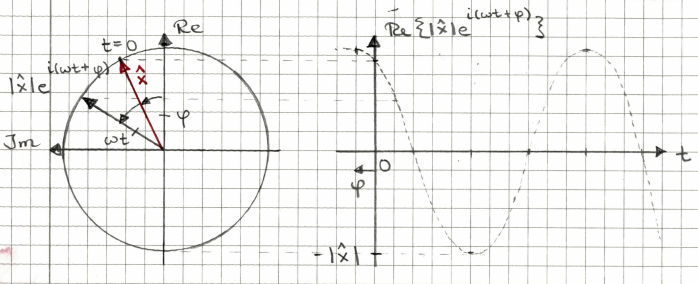
\includegraphics[width=\textwidth]{Bilder/04Einheitskreis.png}
%%	\caption{Einheitskreis und Projektion auf die reelle Achse.}
%%	\label{abb:Einheitskreis}
%%\end{figure}
%
\subsection{Darstellung von Singalen im Zeit- und im Frequenzbereich}
Eine harmonische Schwingung l�sst sich im Frequenzbereich vollst�ndig durch Amplitude $\hat x$, Kreisfrequenz $\Omega$ und Nullphasenwinkel $\varphi$ beschreiben. Diese Eigenschaft motiviert die Darstellung im Zeit- und im Frequenzbereich:
\begin{figure}[H]
	\subfloat[Zeitbereich]{
		\begin{tikzpicture}
			\begin{axis}[
			width=0.3\textwidth,
			height=3.5cm,
			domain=0:2*pi,
			xmin=0,xmax=2*pi,
			grid=both,
			x label style={at={(axis description cs:0.7,-0.1)},anchor=north},
			y label style={at={(axis description cs:-0.1,.5)},rotate=0,anchor=south},
			xlabel={$t$},
			ylabel={$x(t)$}, 
			xtick={0,3.141,6.282},
			xticklabels={0,,$2\pi/\Omega$}, 
			yticklabels={,$-\hat x$,0,$\hat x$}]
			\addplot[black, thick] {cos(deg(x)))};
			\end{axis}
		\end{tikzpicture}
	}
	\subfloat[Frequenzbereich]{
		\begin{tikzpicture}
			\begin{axis}[
			width=0.3\textwidth,
			height=3.5cm,
			xmin=0,xmax=2,ymin=0,ymax=1.8,
			grid=both,
			x label style={at={(axis description cs:0.9,-0.1)},anchor=north},
			y label style={at={(axis description cs:-0.1,.5)},rotate=0,anchor=south},
			xlabel={$\omega$},
			ylabel={Amplitude}, 
			xtick={0,1,2},
			xticklabels={0,$\Omega$,},
			ytick={0,1},
			yticklabels={0,$\hat x$}]
			\addplot[black, thick,mark=*] coordinates { (1,1)};
			\addplot[black, thick] coordinates {(1,0) (1,1)};
			\end{axis}
		\end{tikzpicture}
	}
	\subfloat[Frequenzbereich]{
		\begin{tikzpicture}
		\begin{axis}[
		width=0.3\textwidth,
		height=3.5cm,
		xmin=0,xmax=2,ymin=-1.2,ymax=1.2,
		grid=both,
		x label style={at={(axis description cs:0.9,-0.1)},anchor=north},
		y label style={at={(axis description cs:-0.1,.5)},rotate=0,anchor=south},
		xlabel={$\omega$},
		ylabel={Phase}, 
		xtick={0,1,2},
		xticklabels={0,$\Omega$,},
		ytick={-1,0,1},
		yticklabels={$-\pi$,0,$\pi$}
		]
		\addplot[black, thick,mark=*] coordinates { (1,0)};
		\end{axis}
	\end{tikzpicture}
}
\caption{Reines Cosinussignal $x(t) = \hat{x}\cos (\Omega t) = Re(\hat{x} e^{i \Omega t})$}
\end{figure}
\begin{figure}[H]
	\subfloat[Zeitbereich]{
		\begin{tikzpicture}
		\begin{axis}[
		width=0.3\textwidth,
		height=3.5cm,
		domain=0:2*pi,
		xmin=0,xmax=2*pi,
		grid=both,
		x label style={at={(axis description cs:0.7,-0.1)},anchor=north},
		y label style={at={(axis description cs:-0.1,.5)},rotate=0,anchor=south},
		xlabel={$t$},
		ylabel={$x(t)$}, 
		xtick={0,3.141,6.282},
		xticklabels={0,,$2\pi/\Omega$}, 
		yticklabels={,$-\hat x$,0,$\hat x$}]
		\addplot[black, thick] {sin(deg(x)))};
		\end{axis}
		\end{tikzpicture}
	}
	\subfloat[Frequenzbereich]{
		\begin{tikzpicture}
		\begin{axis}[
		width=0.3\textwidth,
		height=3.5cm,
		xmin=0,xmax=2,ymin=0,ymax=1.8,
		grid=both,
		x label style={at={(axis description cs:0.9,-0.1)},anchor=north},
		y label style={at={(axis description cs:-0.1,.5)},rotate=0,anchor=south},
		xlabel={$\omega$},
		ylabel={Amplitude}, 
		xtick={0,1,2},
		xticklabels={0,$\Omega$,},
		ytick={0,1},
		yticklabels={0,$\hat x$}]
		\addplot[black, thick,mark=*] coordinates { (1,1)};
		\addplot[black, thick] coordinates {(1,0) (1,1)};
		\end{axis}
		\end{tikzpicture}
	}
	\subfloat[Frequenzbereich]{
		\begin{tikzpicture}
		\begin{axis}[
		width=0.3\textwidth,
		height=3.5cm,
		xmin=0,xmax=2,ymin=-1.2,ymax=1.2,
		grid=both,
		x label style={at={(axis description cs:0.9,-0.1)},anchor=north},
		y label style={at={(axis description cs:-0.1,.5)},rotate=0,anchor=south},
		xlabel={$\omega$},
		ylabel={Phase}, 
		xtick={0,1,2},
		xticklabels={0,$\Omega$,},
		ytick={-1,0,1},
		yticklabels={$-\pi$,0,$\pi$}
		]
		\addplot[black, thick,mark=*] coordinates { (1,-0.5)};
		\addplot[black, thick] coordinates { (1,-0.5) (1,0)};
		\end{axis}
		\end{tikzpicture}
	}
	\caption{Reines Sinussignal $x(t) = \hat{x}\sin (\Omega t)  = Re(\hat{x} e^{i (\Omega t-\pi/2)})$}
\end{figure}
\begin{figure}[H]
\subfloat[Zeitbereich]{
	\begin{tikzpicture}
	\begin{axis}[
	width=0.3\textwidth,
	height=3.5cm,
	domain=0:2*pi,
	xmin=0,xmax=2*pi,
	grid=both,
	x label style={at={(axis description cs:0.7,-0.1)},anchor=north},
	y label style={at={(axis description cs:-0.1,.5)},rotate=0,anchor=south},
	xlabel={$t$},
	ylabel={$x(t)$}, 
	xtick={0,3.141,6.282},
	xticklabels={0,,$2\pi/\Omega$}, 
	yticklabels={,$-\hat x$,0,$\hat x$}]
	\addplot[black, thick] {cos(deg(x+pi/3)))};
	\end{axis}
	\end{tikzpicture}
}
\subfloat[Frequenzbereich]{
	\begin{tikzpicture}
	\begin{axis}[
	width=0.3\textwidth,
	height=3.5cm,
	xmin=0,xmax=2,ymin=0,ymax=1.8,
	grid=both,
	x label style={at={(axis description cs:0.9,-0.1)},anchor=north},
	y label style={at={(axis description cs:-0.1,.5)},rotate=0,anchor=south},
	xlabel={$\omega$},
	ylabel={Amplitude}, 
	xtick={0,1,2},
	xticklabels={0,$\Omega$,},
	ytick={0,1},
	yticklabels={0,$\hat x$}]
	\addplot[black, thick,mark=*] coordinates { (1,1)};
	\addplot[black, thick] coordinates {(1,0) (1,1)};
	\end{axis}
	\end{tikzpicture}
}
\subfloat[Frequenzbereich]{
	\begin{tikzpicture}
	\begin{axis}[
	width=0.3\textwidth,
	height=3.5cm,
	xmin=0,xmax=2,ymin=-1.2,ymax=1.2,
	grid=both,
	x label style={at={(axis description cs:0.9,-0.1)},anchor=north},
	y label style={at={(axis description cs:-0.1,.5)},rotate=0,anchor=south},
	xlabel={$\omega$},
	ylabel={Phase}, 
	xtick={0,1,2},
	xticklabels={0,$\Omega$,},
	ytick={-1,0,1},
	yticklabels={$-\pi$,0,$\pi$}
	]
	\addplot[black, thick,mark=*] coordinates { (1,0.3)};
	\addplot[black, thick] coordinates { (1,0.3) (1,0)};
	\end{axis}
	\end{tikzpicture}
}
\caption{Allgemeines Signal $x(t) = \hat{x}\cos (\Omega t+\varphi) = Re(\hat{x} e^{i (\Omega t+\varphi)})$}
\end{figure}
Die �berf�hrung einer harmonischen Funktion vom Zeit- in den Frequenzbereich ist eine �quivalenztransformation. Wird eine allgemeine periodische Funktion als �berlagerung vieler harmonischer Schwingungsanteile mit jeweiliger Kreisfrequenz, Amplitude und Nullphasenwinkel betrachtet, dann kommen in der Darstellung im Frequenzbereich entsprechende Komponenten hinzu. Dies motiviert den n�chsten Abschnitt: 
\section{Darstellung periodischer Funktionen durch Fourierreihen}
Es sei eine $T$-periodische Funktion mit der Grundfrequenz $\Omega = \frac{2\pi}{T}$ gegeben. Unter den Voraussetzungen 
\begin{itemize}
	\item endlich viele Sprungstellen endlicher H�he
	\item 2-Fache Integrierbarkeit von $x(t)$
\end{itemize}
l�sst sich die Funktion $x(t)$ als \emph{Fourierreihe} darstellen:
\begin{theo}[Fourierreihe]{theo:Fourierreihe}
Die Entwicklung von $x(t)$ als Fourierreihe lautet 
\begin{align}
	x(t) = C_0 + \sum_{k=1}^{\infty}C_k \cos (k\Omega t) + S_k \sin (k\Omega t) \nonumber 
\end{align}
wobei die Koeffizienten des Polynoms nach 
\begin{align}
	C_0 & = \frac{1}{T}\int_{-T/2}^{T/2}x(t) \textrm{d}t \nonumber\\
	C_k & = \frac{2}{T}\int_{-T/2}^{T/2}x(t)\cos(k\Omega t)\textrm{d}t& 
	&k\in \mathbb{N}&\nonumber\\
	S_k & = \frac{2}{T}\int_{-T/2}^{T/2}x(t)\sin(k\Omega t)\textrm{d}t& 
	&k\in \mathbb{N}&\nonumber
\end{align}
berechnet werden. 
\end{theo}
Alternativ gelten auch die folgenden Darstellungen:\\
\begin{theo}[Darstellung der Fourierreihe durch Amplitude und Phase]{theo:FourierreiheAmpPha}
\begin{align}
x(t) = C_0 + \sum_{k=1}^{\infty}\hat x_k \cos (k\Omega t+\varphi_k) \nonumber 
\end{align}
Die Folge $\hat x_1$, $\hat x_2$,... hei�t \emph{Amplitudenspektrum}, die Folge  $\varphi_1$, $\varphi_2$, ... hei�t \emph{Phasenspektrum}. Man spricht auch von der Spektraldarstellung der Funktion $x(t)$. 
\end{theo}
\begin{theo}[Darstellung der Fourierreihe als komplexes Polynom]{theo:Fourierreihekomplex}
		\begin{align}
		x(t) = \sum_{k=-\infty}^{\infty} a_k e^{i k\Omega t} \nonumber 
		\end{align}
		wobei die Koeffizienten des Polynoms nach 
		\begin{align}
		a_k & = \frac{1}{T}\int_{0}^{T}x(t)e^{-i k\Omega t}\textrm{d}t & 
		&k\in \{-n,n\}, n\in \mathbb{N}&\nonumber 
		\end{align}
		berechnet werden. 
\end{theo}
Anmerkungen: 
\begin{itemize}
	\item Die Darstellung der Funktion $x(t)$ als Fourierreihe bietet den Vorteil der Zerlegung in einzelne Frequenzanteile
	\item Der Anteil $\hat x_1\cos (\Omega t+\varphi_1)$ hei�t \emph{Grundschwingung} oder \emph{1. Harmonische}
	\item Der Anteil $\hat x_2\cos (2\Omega t+\varphi_2)$ hei�t \emph{1. Oberschwingung} oder \emph{2. Harmonische}
	\item Der Anteil $\hat x_k\cos (k \Omega t+\varphi_k)$ hei�t \emph{(k-1)-te Oberschwingung} oder \emph{k-te Harmonische}
	\item Bei der Berechnung der Fourierkoeffizienten muss nicht zwingend auf $t\in [-T/2, T/2]$ integriert werden. Wichtig ist, dass eine Periode vollst�ndig abgedeckt ist: Es muss gelten $t\in [t_0, t_0 + T]$ f�r beliebige $t_0$. 
	\item Periodische Funktionen k�nnen durch eine endliche Zahl von Elementen ihrer Fourierreihe approximiert werden. Der Fehler konvergiert im quadratischen Mittel. 
\end{itemize}
%\subsection{Berechnung der Fourierkoeffizienten bei symmetrischen Funktionen}
Es gelten insbesondere die zwei Spezialf�lle: 
\paragraph{Gerade Funktionen.} F�r gerade Funktionen $x(t)$ gilt $x(t)=x(-t)$. Dann folgt: 
\begin{align}
	&S_k = 0&
	&C_k = \frac{4}{T}\int_{0}^{T/2} x(t) \cos (k\Omega t) \textrm{d}t&
\end{align}
\paragraph{Ungerade Funktionen.} F�r ungerade Funktionen $x(t)$ gilt $x(t)=-x(-t)$. Dann folgt: 
\begin{align}
&S_k = \frac{4}{T}\int_{0}^{T/2} x(t) \sin (k\Omega t) \textrm{d}t&
&C_k = 0&
\end{align}
\begin{beispiel}[Rechteckschwingung]{beispiel:Rechteckschwingung}
Das Rechtecksignal ist definiert als 
\begin{align}
	x(t) = \left\{
	\begin{array}{ll}
		-1 & \frac{-T}{2} \leq t \leq 0\\
		1 & 0\leq t \leq \frac{T}{2}\\
	\end{array}
	\right. 
\end{align}
Die Grundfrequenz ist $\Omega=2\pi/T$. Diese Funktion ist punktsymmetrisch zum Ursprung, also ungerade. Daher ist
\begin{align}
	C_k&=0, k\in \mathbb N_0,\\
	S_k&=\frac{4}{T}\int_{0}^{T/2}x(t)\sin(k\Omega t)\textrm{d}t\\
	& =-\frac{4}{T k \Omega}\left(\cos\left(k\Omega \frac{T}{2}\right)-1\right)\\
	& = \frac{2}{k \pi}\left(1-(-1)^k\right)\\
	& = \left\{
	\begin{array}{ll}
		0 & k \textrm{ gerade}\\
		\frac{4}{k \pi} & k \textrm{ ungerade}\\
	\end{array}
	\right. 	
\end{align}
Die Reihenentwicklung der Rechteckfunktion $x(t)=\sum_{k} S_k \sin (k\Omega t)$ hat wegen $x(t)= \sum_{k} S_k \cos (k\Omega t-\pi/2)$ die Amplituden $\hat x_k=S_k$ und die Phasen $\varphi_k =-\pi/2$. Die Darstellung im Zeit- und im Frequenzbereich ist wie folgt: 
\begin{figure}[H]
	\subfloat[Zeitbereich]{
		\begin{tikzpicture}
		\begin{axis}[
		width=0.3\textwidth,
		height=3.5cm,
		domain=-1:7,
		xmin=-0.2,xmax=2*pi+0.2,
		grid=both,
		x label style={at={(axis description cs:0.7,-0.1)},anchor=north},
		y label style={at={(axis description cs:-0.1,.5)},rotate=0,anchor=south},
		xlabel={$t$},
		ylabel={$x(t)$}, 
		xtick={0,3.141,6.282},
		xticklabels={0,,$2\pi/\Omega$}, 
		%yticklabels={,$-\hat x$,0,$\hat x$}
		]
		\addplot[black, thick] coordinates {(-1,-1) (0,-1) (0,1) (3.141,1) (3.141,-1) (6.242,-1) (6.242,1) (6.5,1)};
		\end{axis}
		\end{tikzpicture}
	}
	\subfloat[Frequenzbereich]{
		\begin{tikzpicture}
		\begin{axis}[
		width=0.3\textwidth,
		height=3.5cm,
		%		xmin=0,xmax=2,ymin=0,ymax=1.8,
		grid=both,
		x label style={at={(axis description cs:0.9,-0.1)},anchor=north},
		y label style={at={(axis description cs:-0.1,.5)},rotate=0,anchor=south},
		xlabel={$\omega/\Omega$},
		ylabel={$S_k\cdot \pi/4$}, 
		xtick={1,3,5,7},
		%		xticklabels={0,$\Omega$,},
		ytick={0,1},
		%		yticklabels={0,$\hat x$}
		]
		\addplot[black, thick,mark=*,only marks] coordinates {(1,1) (2,0) (3,1/3) (4,0) (5,1/5) (6,0) (7,1/7)};
		%		\addplot[black, thick] coordinates {(1,0) (1,1)};
		\end{axis}
		\end{tikzpicture}
	}
	\subfloat[Frequenzbereich]{
		\begin{tikzpicture}
		\begin{axis}[
		width=0.3\textwidth,
		height=3.5cm,
		ymin=-3.2,ymax=0.2,%ymin=-1.2,ymax=1.2,
		grid=both,
		x label style={at={(axis description cs:0.9,-0.1)},anchor=north},
		y label style={at={(axis description cs:-0.15,.85)},rotate=0,anchor=south},
		xlabel={$\omega/\Omega$},
		ylabel={$\varphi_k$}, 
		xtick={1,3,5,7},
		%		xticklabels={0,$\Omega$,},
		ytick={-3.141,-1.505,0},
		yticklabels={$-\pi$,$-\pi/2$,$0$}
		]
		\addplot[black, thick,mark=*,only marks] coordinates {(1,-1.505) (2,0) (3,-1.505) (4,0) (5,-1.505) (6,0) (7,-1.505)};
		\end{axis}
		\end{tikzpicture}
	}
\end{figure}
Die Amplituden der $k$-ten Harmonischen fallen mit $\frac{1}{k}$ ab. Aufgrund der steilen Flanken der Rechteckfunktion spielen h�here Harmonische eine wichtige Rolle bei der Konvergenz der Reihe. Wegen der Unstetigkeit im Zeitverlauf tritt das \emph{Gibbs'sche Ph�nomen} auf, das zum �berschwingen der Fourierentwicklung gegen�ber der Rechteckfunktion f�hrt. 
\begin{figure}[H]
	\centering
	\begin{tikzpicture}
		\begin{axis}[
		width=0.6\textwidth,
		height=0.3\textwidth,
		domain=-1:7,
		xmin=-0.2,xmax=2*pi+0.2,
		grid=both,
		x label style={at={(axis description cs:0.7,-0.1)},anchor=north},
		y label style={at={(axis description cs:-0.1,.5)},rotate=0,anchor=south},
		xlabel={$t$},
		ylabel={$x(t)$}, 
		xtick={0,3.141,6.282},
		xticklabels={0,,$2\pi/\Omega$}, 
		yticklabels={,$-\hat x$,0,$\hat x$}]
		\addplot[black, thick] coordinates {(-1,-1) (0,-1) (0,1) (3.141,1) (3.141,-1) (6.242,-1) (6.242,1) (6.5,1)};
		\addplot[blue, thick,samples=200] {sin(deg(x))*4/pi + sin(3*deg(x))*4/pi/3 + sin(5*deg(x))*4/pi/5};
		\addplot[red, thick,samples=400] {sin(deg(x))*4/pi + sin(3*deg(x))*4/pi/3 + sin(5*deg(x))*4/pi/5+sin(7*deg(x))*4/pi/7+sin(9*deg(x))*4/pi/9+sin(11*deg(x))*4/pi/11+sin(13*deg(x))*4/pi/13+sin(15*deg(x))*4/pi/15};
		\legend{Rechteck,$k=5$,$k=15$}
		\end{axis}
	\end{tikzpicture}
\end{figure}
\end{beispiel}
\begin{beispiel}[Rechteckimpulsfolge]{beispiel:Rechteckimpulsfolge}
Eine Rechteckimpulsfolge ist definiert als die periodische Abfolge von Rechteckimpulsen. Die Periode sei gegeben durch $T$, die Impulsl�nge durch $\tau$. Analog zum Dirac-Sto� hat die Fl�che des Sto�es per Definition den Wert 1. 
\begin{figure}[H]
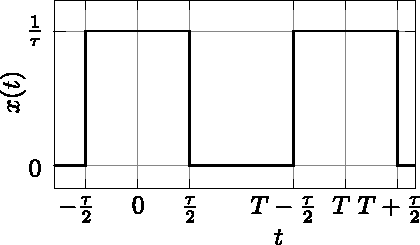
\includegraphics[width=0.5\textwidth]{Bilder/04Rechteckimpulsfolge.pdf}
\end{figure}
Es liegt eine gerade Funktion vor. Die Berechnung der Fourierkoeffizienten liefert
\begin{align}
S_k&=0, k\in \mathbb N_0,\\
C_0&=\frac{1}{T}\int_{0}^{T/2}x(t)\textrm{d}t = \frac{1}{T}\\
C_k& =\frac{2}{T}\int_{0}^{T}x(t)\cos (k \Omega t)\textrm{d}t =\frac{2}{T}\left(\int_{-\tau/2}^{\tau/2}\frac{1}{\tau}\cos (k \Omega t)\textrm{d}t +\int_{\tau/2}^{T-\tau/2}0\textrm{d}t\right)\\
& =2\cdot \frac{2}{T k \Omega}\frac{1}{\tau}\left(\sin\left(k\Omega \frac{\tau}{2}\right)\right)\\
&= \frac{2}{k\pi \tau}\sin\left(k\pi\frac{\tau}{T}\right)
\end{align}
Somit lautet die Fourierreihe der Rechteckimpulsfolge
\begin{align}
	x(t) = \frac{1}{T} + \sum_{k=1}^{\infty}\frac{2}{k\pi \tau}\sin\left(k\pi \frac{\tau}{T}\right)\cos (k\Omega t)
\end{align}
Der Sto�charakter wird unterschieden nach Verh�ltnis von $\tau$ und $T$: Bei einem kleinen Wert von $\tau$ (kurzer Sto�dauer) ist die Amplitude $\frac{2}{k\pi\tau}$ gro�. Die erste Nullstelle der $C_k$ liegt bei $\frac{\tau}{T}=\frac{1}{k}$. Es liegt viel Energie bei hohen Frequenzen vor. Man spricht vom \emph{harten Sto�}. Im Gegensatz dazu kommt die erste Nullstelle der $C_k$ umso fr�her, je gr��er das Verh�ltnis $\tau/T$. Es liegt viel Energie bei den kleinen Frequenzen. Die Verteilung der Amplituden in Abh�ngigkeit der Frequenz ist in der folgenden Abbildung zu sehen. 
\begin{figure}[H]
	\centering
	\begin{tikzpicture}
	\begin{axis}[
	width=0.6\textwidth,
	%		height=3.5cm,
	domain=1:20,
	xmin=1,xmax=20,
	grid=both,
	x label style={at={(axis description cs:0.7,-0.1)},anchor=north},
	y label style={at={(axis description cs:-0.1,.5)},rotate=0,anchor=south},
	xlabel={$k$},
	ylabel={$C_k$}, 
	]
	\addplot[blue, thick,samples=20, mark=*, only marks] {abs(2*sin(deg(x*0.25*pi))/(x*0.25*pi))};
	\addplot[red, thick,samples=20, mark=*, only marks] {abs(2*sin(deg(x*0.07*pi))/(x*0.07*pi))};
	\legend{weicher Sto� ($\tau/T=0.25$),harter Sto� ($\tau/T=0.07$)}
	\end{axis}
	\end{tikzpicture}
	\caption{Harter und weicher Sto�.}
%	\label{abb:HarterWeicherSto�}
\end{figure}
\end{beispiel}
\begin{beispiel}[Dreieckschwingung]{beispiel:Dreieckschwingung}
Die Dreieckschwingung ist definiert als 
\begin{align}
x(t) = \left\{
\begin{array}{ll}
t\cdot \frac{4}{T} & -\frac{T}{4} \leq t \leq \frac{T}{4}\\
2-t \cdot \frac{4}{T} &  \frac{T}{4} \leq t \leq \frac{3 T}{4}\\
\end{array}
\right. 
\end{align}
Auch diese Funktion ist ungerade, weshalb die Koeffizienten $C_k$ allesamt verschwinden. Ferner ist 
\begin{align}
S_k&=\frac{4}{T}\int_{0}^{T/2}x(t)\sin(k\Omega t)\textrm{d}t\\
& = \left\{
\begin{array}{ll}
0 & k \textrm{ gerade}\\
\frac{8}{k^2 \pi^2}\cdot (-1)^{(k-1)/2} & k \textrm{ ungerade}\\
\end{array}
\right. 	
\end{align}
Die Darstellung von Zeitsignal, Amplituden- und Phasenspektrum ist wie folgt: 
\begin{figure}[H]
	\subfloat[Zeitbereich]{
		\begin{tikzpicture}
		\begin{axis}[
		width=0.3\textwidth,
		height=3.5cm,
		domain=-1:7,
		xmin=-0.2,xmax=2*pi+0.2,
		grid=both,
		x label style={at={(axis description cs:0.7,-0.1)},anchor=north},
		y label style={at={(axis description cs:-0.1,.5)},rotate=0,anchor=south},
		xlabel={$t$},
		ylabel={$x(t)$}, 
		xtick={0,3.141,6.282},
		xticklabels={0,,$2\pi/\Omega$}, 
		%yticklabels={,$-\hat x$,0,$\hat x$}
		]
		\addplot[black, thick] coordinates {(0,0) (1.5705,1) (3.141,0) (4.712,-1) (6.242,0) };
		\end{axis}
		\end{tikzpicture}
	}
	\subfloat[Frequenzbereich]{
		\begin{tikzpicture}
		\begin{axis}[
		width=0.3\textwidth,
		height=3.5cm,
		%		xmin=0,xmax=2,ymin=0,ymax=1.8,
		grid=both,
		x label style={at={(axis description cs:0.9,-0.1)},anchor=north},
		y label style={at={(axis description cs:-0.1,.5)},rotate=0,anchor=south},
		xlabel={$\omega/\Omega$},
		ylabel={$S_k\cdot \pi^2/8$}, 
		xtick={1,3,5,7},
		%		xticklabels={0,$\Omega$,},
		ytick={0,1},
		%		yticklabels={0,$\hat x$}
		]
		\addplot[black, thick,mark=*,only marks] coordinates {(1,1) (2,0) (3,1/9) (4,0) (5,1/25) (6,0) (7,1/49)};
		%		\addplot[black, thick] coordinates {(1,0) (1,1)};
		\end{axis}
		\end{tikzpicture}
	}
	\subfloat[Frequenzbereich]{
		\begin{tikzpicture}
		\begin{axis}[
		width=0.3\textwidth,
		height=3.5cm,
		ymin=-1.7,ymax=1.7,%ymin=-1.2,ymax=1.2,
		grid=both,
		x label style={at={(axis description cs:0.9,-0.1)},anchor=north},
		y label style={at={(axis description cs:-0.15,.7)},rotate=0,anchor=south},
		xlabel={$\omega/\Omega$},
		ylabel={$\varphi_k$}, 
		xtick={1,3,5,7},
		%		xticklabels={0,$\Omega$,},
		ytick={-1.505,0,1.505},
		yticklabels={$-\pi/2$,$0$,$\pi/2$}
		]
		\addplot[black, thick,mark=*,only marks] coordinates {(1,-1.505) (2,0) (3,1.505) (4,0) (5,-1.505) (6,0) (7,1.505)};
		\end{axis}
		\end{tikzpicture}
	}
\end{figure}
\end{beispiel}
\section{Erzwungene Schwingungen mit periodischer Anregung}
Es wird der ged�mpfte Einmassenschwinger (Parameter $m$, $d$, $c$) mit periodischer Krafterregung $F(t)$ betrachtet. Die Krafterregung sei jetzt \emph{polyharmonisch}, d.h. sie setzt sich aus vielen Frequenzanteilen zusammen. Dies ist beispielsweise bei Rechtecks- oder Dreiecksanregung der Fall. Die allgemeine Darstellung sei als Fourierreihe gegeben: 
\begin{align}
	F(t) = \frac{F_0}{2} +\sum_{k=1}^{\infty} F_{C,k}\cos(k\Omega t) + F_{S,k}\sin(k\Omega t)
\end{align}
Somit lautet die DGL
\begin{align}
m\ddot x + d\dot x + c x = \frac{F_0}{2} +\sum_{k=1}^{\infty} F_{C,k}\cos(k\Omega t) + F_{S,k}\sin(k\Omega t)
\end{align}
Die Antwort $x(t)$ kann f�r drei isolierte F�lle separat betrachtet werden: 
\paragraph{Fall 1: $k=0$.} Die Anregung $F_1(t)=F_0/2$ ist konstant; die Antwort darauf (partikul�re L�sung) kann durch einen Ansatz vom Typ der rechten Seite bestimmt werden: 
\begin{align}
	&x_1(t) = K \textrm{ (konstant)}&&\dot x(t)=0&&\ddot x(t)=0& 
\end{align}
Nach kurzer Umformung folgt 
\begin{align}
x_1(t) = K = \frac{F_0}{2 c}
\end{align}
\paragraph{Fall 2: $k\geq 1$, $F_{S,k}=0$.} Die Anregung durch eine Drehzahlvielfache lautet $F_2(t)=F_{C,k}\cos(k\Omega t)$. Die Antwort darauf (partikul�re L�sung) lautet 
\begin{align}
x_2(t) &= V\left(\frac{k\Omega}{\omega_0}\right)\frac{F_{C,k}}{c}\cos\left(k\Omega t+\varphi_k\right)\\
V\left(\frac{k\Omega}{\omega_0}\right) &= \frac{1}{\sqrt{\left(1-\left(\frac{k\Omega}{\omega_0}\right)^2\right)^2+\left(2D\frac{k\Omega}{\omega_0}\right)^2}}\\
&= \frac{1}{\sqrt{\left(1-\left(k\eta\right)^2\right)^2+\left(2Dk\eta\right)^2}}
\end{align}
\begin{align}
\tan(\varphi_k) &= - \frac{2D\frac{k\Omega}{\omega_0}}{1-\left(\frac{k\Omega}{\omega_0}\right)^2} 
= -\frac{2Dk\eta}{1-\left(k\eta\right)^2}
\end{align}
\paragraph{Fall 3: $k\geq 0$ $F_{C,k}=0$.} Die Anregung durch eine Drehzahlvielfache lautet $F_3(t)=F_{C,k}\sin(k\Omega t)$. Die Antwort darauf (partikul�re L�sung) lautet in Analogie zu Fall 2
\begin{align}
x_3(t) &= V\left(\frac{k\Omega}{\omega_0}\right)\frac{F_{C,k}}{c}\sin\left(k\Omega t+\varphi_k\right)
\end{align}
Gem�� dem Superpositionsprinzip ist die Schwingungsantwort auf die Einzelanregungen $F(t) = F_1(t) + F_2(t) + F_3(t)$ die Summe der Einzelantworten $x(t) = x_1(t) + x_2(t) + x_3(t)$, also 
\begin{align}
x(t) = \frac{F_0}{2c} + \sum_{k=1}^{\infty}V\left(\frac{k\Omega}{\omega_0}\right)\left(\frac{F_{C,k}}{c}\cos\left(k\Omega t+\varphi_k\right) + \frac{F_{S,k}}{c}\sin\left(k\Omega t+\varphi_k\right)\right)
\label{eq:PolyH}
\end{align}
Diese L�sung hat Eigenschaften wie die Schwingungsantwort auf eine Einzelanregung. Die Resonanz des unged�mpften Einmassenschwingers wird jetzt nicht mehr nur bei $\Omega=\omega_0$, sondern bei $k \Omega=\omega_0$ mit allen $k\in \mathbb N$ angeregt. 
\begin{beispiel}[Motorblockanregung]{beispiel:Motorblockanregung}
Die Vertikalbewegung eines Motorblocks kann durch die bekannte DGL des 1-Massen-Schwingers beschrieben werden. Die Schwingungsanregung durch Z�ndung der 4 Zylinder hat ihre Hauptkomponente bei doppelter Motordrehzahl, eine weitere wichtige Komponente ist die 4. Dehzahlordnung. Wenn die Anregung vereinfachend konstante Amplituden hat, dann lautet die Bewegungsgleichung 
\begin{align}
	m\ddot x + d\dot x + c x = F_{C,2} \cos(2 \Omega t) + F_{C,4} \cos(4 \Omega t)
\end{align}
Gem�� Gleichung (4.41) lautet die partikul�re L�sung
\begin{align}
x(t) = & V_{Kraftanregung}\left(\frac{2\Omega}{\omega_0}\right)\frac{F_{C,2}}{c}\cos\left(2\Omega t+\varphi_2\right) \\
&+V_{Kraftanregung}\left(\frac{4\Omega}{\omega_0}\right)\frac{F_{C,4}}{c}\cos\left(2\Omega t+\varphi_4\right) 
\end{align}
Diese Aufgabe kann numerisch gel�st werden. In \emph{Octave} lautet eine m�gliche Implementierung 
\begin{lstlisting}[frame=single] 
function dy = Motorblock(t,y)
m = 1; d = 5; c = 1e4*(2*pi)^2;
Fc2 = 1; Fc4 = 0.5; 

Omega = t*500*2*pi/60; % Drehzahlhochlauf (500 rpm 
                       % pro Sekunde)
Phi = 1/2*Omega*t; 

dy = zeros(size(y)); 
dy(1) = y(2); 
dy(2) = (-c*y(1)-d*y(2) + Fc2*cos(2*Phi) + Fc4*cos(4*Phi))/m; 
\end{lstlisting}
\begin{lstlisting}[frame=single] 
% main function
close all; clear variables; clc;
tspan = linspace(0,10,10000);
y0 = [0,0];
[tout,yout] = ode45(@Motorblock,tspan,y0);
figure, plot(tout,yout(:,1)); 

Fs=length(tout)/(tout(end)-tout(1));
step=ceil(50*Fs/1000); window=ceil(500*Fs/1000);
[s,f,t] = specgram(yout(:,1), 2^10, Fs,window, window-step);
[t,f] = meshgrid(t,f);
figure, surf(t,f,abs(s),'edgecolor','none');
caxis([0.0 1e-3]); axis([0 10 10 200 0 1e-2]); 
\end{lstlisting}
\begin{figure}[H]
%	\centering
	\subfloat{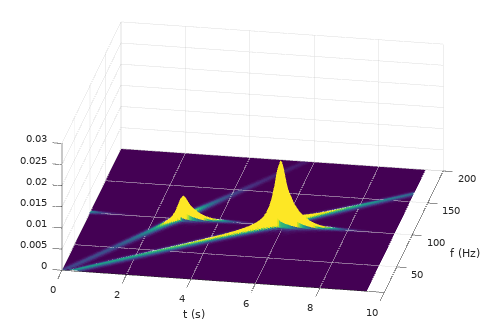
\includegraphics[width=0.5\textwidth]{Bilder/Hochlaufsimulation_Farbkarte.png}}
	\subfloat{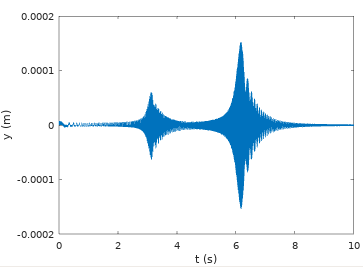
\includegraphics[width=0.4\textwidth]{Bilder/Hochlaufsimulation_y.png}}
	\caption{Spektrogramm der Auslenkung $y(t)$ bei Hochlaufsimulation und Anregung mit 2. und 4. Ordnung. Charakteristisch sind im Spektrogramm die Anregungsordnungen, mit denen die Resonanz jeweils getroffen wird. }
\end{figure}
\end{beispiel}
\section{Nichtperiodische Vorg�nge}
F�r periodische Funktionen gilt: $\Omega = \frac{2\pi}{T}$. Die Grundfrequenz ist also durch die endliche Periodenl�nge begrenzt. F�r nichtperiodische Funktionen (z.B. einmalige Vorg�nge) geht die Schwingungsdauer $T$ gegen unendlich. Damit ist auch die Grundfrequenz $\Omega\rightarrow \textrm{d}\omega$ (sie wird differenziell klein) bzw. $k\Omega\rightarrow\omega$. Mit Darstellung von (Mathematik 4.5) lauten die komplexen Schwingungskomponenten im Grenz�bergang
\begin{align}
x(t) &= \sum_{k=-\infty}^{\infty}a_k e^{i k\Omega t} = \sum_{k=-\infty}^{\infty}\frac{1}{T}\underbrace{\int_{0}^{T}x(t)e^{-i k\Omega t}\textrm{d}t}_{=: X_k = X(k\Omega)} e^{i k\Omega t}\\
&\rightarrow \frac{1}{2\pi}\int_{-\infty}^{\infty}\underbrace{\int_{0}^{\infty}x(t)e^{-i \omega t}\textrm{d}t}_{X(\omega)} e^{i \omega t}\textrm{d}\omega
\end{align}
Dies motiviert die folgende Definition:
\begin{theo}[Fouriertransformation]{theo:Fouriertransformation}
Die Fouriertransformation $\mathcal{F}(x)$ beschreibt die Transformation einer Funktion $x(t)$ in den Frequenzbereich. Sie ist definiert durch 
\begin{align}
X(\omega) = \mathcal F \{x(t)\}&= \int_{0}^{\infty} x(t)e^{-i \omega t}\textrm{d}t \nonumber
\end{align}
Die R�cktransformierte $x(t) = \mathcal{F}^{-1}\{X(\omega)\}$ wird berechnet als 
\begin{align}
x(t) = \frac{1}{2\pi}\int_{-\infty}^{\infty} X(\omega)e^{i \omega t}\textrm{d}\omega\nonumber
\end{align}
\end{theo}
Der Betrag $|X(\omega)|$ beschreibt das Amplitudenspektrum der nichtperiodischen Funktion $x(t)$. Es gilt der Zusamenhang zwischen Amplitude und Phase
\begin{align}
	X(\omega) &= |X(\omega)| e^{i\varphi(\omega)} =  Re\{X(\omega)\} +i\cdot Re\{X(\omega)\}\\
	\tan (\varphi(\omega)) & = \frac{Im\{X(\omega)\}}{Re\{X(\omega)\}}
\end{align}
In der Definition der Fouriertransformierten in (Mathematik 4.6) wurde angenommen, dass die aperiodischen Signale f�r $t<0$ den Wert $0$ haben. Um den Fall $x(t<0)\neq 0$ abzudecken, lautet die verallgemeinerte Fouriertransformierte
\begin{align}
	X(\omega)&= \int_{-\infty}^{\infty} x(t)e^{-i \omega t}\textrm{d}t
\end{align}
Die R�cktransformierte bleibt unver�ndert. F�r die Fouriertransformation gelten die folgenden Rechenregeln: 
\begin{itemize}
	\item Linearit�t
\begin{align}
\mathcal{F}\{c_1 x_1(t) + c_2 x_2(t)\} = c_1 X_1(\omega) + c_2 X_2(\omega)
\end{align}
	\item Differentiation im Urbildraum
\begin{align}
\mathcal{F}\left\{\frac{d^n x(t)}{\textrm{d} t}\right\} = (i \omega)^n X(\omega) - x(0^+)
\end{align}
mit der Anfangsbedingung $x(0^+)$, welche bei homogenen Anfangsbedingungen verschwindet.
\end{itemize}
\begin{beispiel}[Dirac-Impuls]{beispiel:Diracimpuls}
Die Fouriertransformierte des Dirac-Impuls berechnet sich unter Ber�cksichtigung der Ausblendeigenschaft zu  
\begin{align}
	\mathcal{F}(\delta(t))&=\int_{-\infty}^{\infty}\delta(t)e^{-i\omega t}\textrm{d}t = e^{-i\omega \cdot 0} = 1
\end{align}
Ein Dirac-Impuls ist ein unendlich harter Sto�. Folglich befinden sich in dessen Amplitudenspektrum alle Frequenzen mit der Spektraldichte 1. Man spricht von \emph{wei�em Rauschen}. 	
\end{beispiel}
\begin{beispiel}[Sprungfunktion]{beispiel:Sprung}
Die Fouriertransformierte der Sprungfunktion berechnet sich wegen $\delta (t) = \textrm{d}\sigma(t)/\textrm{d}t$ und 
\begin{align}
\mathcal{F}(\delta(t))&=i\omega \mathcal{F}(\sigma(t))-\delta(0^+)=i\omega \mathcal{F}(\sigma(t))
\end{align}
zu 
\begin{align}
\mathcal{F}(\sigma(t))&=\frac{1}{i\omega }
\end{align}
\end{beispiel}
\begin{beispiel}[Harmonische Funktion]{beispiel:harmonisch}
\begin{align}
\mathcal{F}(\sin(\Omega t)) &= i \pi \left(\delta(\omega+\Omega)-\delta(\omega-\Omega)\right)\\
\mathcal{F}(\cos(\Omega t)) &= \pi \left(\delta(\omega-\Omega)+\delta(\omega+\Omega)\right)
\end{align}
\end{beispiel}
\begin{beispiel}[Rechteckimpuls ohne Wiederholung]{beispiel:ImpulsOhneWdh}
In Analogie zur Rechteckimpulsfolge wird der einmalige Rechteckimpuls ohne Wiederholung, d.h. mit $T\rightarrow\infty$, im Frequenzbereich betrachtet. Daf�r eignet sich die Fouriertransformation: 
\begin{align}
	X(\omega) &= \int_{-\tau/2}^{\tau/2}\frac{1}{\tau}e^{-i\omega t}\textrm{d}t = \frac{e^{i\omega\tau/2}-e^{-i\omega\tau/2}}{i\tau\omega} = \frac{2}{\tau \omega}\sin(\omega\tau /2)
\end{align}
Bemerkenswert an diesem Ergebnis sind zwei Beobachtungen: Das bisherige diskrete Frequenzspektrum (Grundfrequenz $\Omega$) geht nun �ber in ein verteiltes Spektrum, f�r das alle reellen Werte von $\omega$ zugelassen sind; die weiteren Eigenschaften des bisherigen Ergebnisses sind beibehalten. Ferner folgt f�r den Grenz�bergang $\tau\rightarrow0$ das Ergebnis von Beispiel 4.5. 
\begin{figure}[H]
	\centering
	\begin{tikzpicture}
	\begin{axis}[
	width=0.6\textwidth,
	height=4cm,
	domain=1:20,
	xmin=1,xmax=20,
	grid=both,
	x label style={at={(axis description cs:0.7,-0.3)},anchor=north},
	y label style={at={(axis description cs:-0.1,.5)},rotate=0,anchor=south},
	xlabel={$\omega$},
	ylabel={$|X(\omega)|$}, 
	]
	\addplot[black, thick,samples=200] {abs(2*sin(deg(x*0.5)/2)/x/0.5)};
	\end{axis}
	\end{tikzpicture}
\end{figure}
\end{beispiel}\newpage
\begin{beispiel}[Impulsantwort des Einmassenschwingers]{beispiel:HarmOsz}
Die Fouriertransformation angewandt auf die Gleichung (4.3) lautet gem�� der Rechenregeln: 
\begin{align}
	-\omega^2 X(\omega) + 2Di\omega X(\omega)+\omega_0^2 X(\omega)& =\frac{1}{m}\mathcal{F}\{\delta(t)\}=\frac{1}{m}&&\textrm{bzw.}&\label{eq:GImpuls}\\
	X(\omega)& = \frac{1}{m}\frac{1}{\left(\omega_0^2-\omega^2 + 2Di\omega \right)}&
\end{align}
\end{beispiel}
Diese Darstellung der Fouriertransformierten erinnert stark an die komplexe Darstellung der �bertragungsfunktion und motiviert den n�chsten Abschnitt: 
\section{Berechnung der Schwingungsantwort mithilfe des komplexen Frequenzgangs}
Als Ausgangspunkt wird ein lineares System mit zeitunabh�ngigen Parametern und einer allgemeinen Eingangsgr��e $y(t)$ gew�hlt. Die Anwendung der Fouriertransformation auf die Differentialgleichung 
\begin{align}
& \sum_{k=0}^{n} a_k \frac{\textrm{d}^k x}{\textrm{d} t^k} = b_0 y& &n\in \mathbb N&
\end{align}
lautet 
\begin{align}
\left(\sum_{k=0}^{n} a_k \cdot (i\omega)^k \right) X(\omega) = b_0 Y(\omega)
\end{align}
Ferner wird die �bertragungsfunktion 
\begin{align}
G(\omega)=\frac{X(\omega)}{Y(\omega)} = \frac{b_0}{\sum_{k=0}^{n} a_k \cdot (i\omega)^k }
\end{align}
eingef�hrt, welche im Frequenzbereich den Zusammenhang zwischen Einheitsanregung und Antwort herstellt. \\
Wie im (Beispiel 4.9) ersichtlich, folgt aus der \emph{Einheitsanregung} $y(t)=\delta(t)$ im Frequenzbereich die �bertragungsfunktion. Au�erdem ist die �bertragungsfunktion $G(\omega)$ auch aus der Fouriertransformation der Impulsantwort $g(t)$ berechenbar: $\mathcal{F}\left\{\frac{1}{m\omega_d}e^{-D\omega_0 t}\sin(\omega_d t)\right\} = \frac{1}{m}\frac{1}{\left(\omega_0^2-\omega^2 + 2Di\omega \right)}$. Diese Beobachtung ist allgemein g�ltig: Es ist stets 
\begin{align}
	\mathcal{F}\left\{g(t)\right\} = G(\omega)
\end{align}
Die �bertragungsfunktion $G(\omega)$ beschreibt ein lineares zeitinvariantes System vollst�ndig. Ist sie bekannt, dann kann die Antwort auf eine beliebige Anregung im Frequenzbereich berechnet werden. Die R�cktransformation liefert die Schwingungsantwort im Zeitbereich: mit $X(\omega) = G(\omega) Y(\omega)$ ist 
\begin{align}
	\mathcal{F}\left\{x(t)\right\} &=X(\omega)= G(\omega) Y(\omega) = \int_{-\infty}^{\infty}g(z)e^{-i\omega t}\textrm{d}t \cdot \int_{-\infty}^{\infty}y(t)e^{-i\omega t}\textrm{d}t\\
	& = \int_{-\infty}^{\infty}\int_{-\infty}^{\infty}g(t-\tau)y(\tau)\textrm{d}\tau \cdot e^{-i\omega t}\textrm{d}t\\
	&= \mathcal{F}\left\{g(t)*y(t)\right\} 
\end{align}
mit 
\begin{align}
	g(t)*y(t) := \int_{-\infty}^{\infty}g(t-\tau)y(\tau)\textrm{d}\tau
\end{align}
der \emph{Faltung} zwischen der Gewichtsfunktion und einer beliebigen Anregungsfunktion. \\\newpage
\section*{Aufgaben zu Kapitel 4}
\paragraph{4.1} Berechnen Sie die Koeffizienten $C_0$, $C_k$ und $S_k$ der folgenden Funktionen: 
\begin{align}
	&\textrm{a.}& &f(t) = a \sin(\omega_0 t) + b \cos(2\omega_0 t), &&t\in [{0,2\pi/\omega_0}]& \\
	&\textrm{b.}& &f(t) = a \sin^2(\omega_0 t)-\cos(\omega_0 t),&&t\in [{0,2\pi/\omega_0}]& \\
	&\textrm{c.}& &f(t) = c + a \sin(\omega_0 t) + b \sin(\omega_0 t)\cos(\omega_0 t),&& t\in [{0,2\pi/\omega_0}]& \\
	&\textrm{d.}& &f(t) = \sigma(t) - \sigma(t-1),&& t\in [{0,2}]& \\
	&\textrm{d.}& &f(t) = t \cdot \sigma(t) + (1-t) \cdot \sigma(t-1),&& t\in [{0,2}]& 
\end{align}
\paragraph{4.2} Berechnen Sie die Koeffizienten $a_k$ der folgenden Funktionen: 
\begin{align}
	&\textrm{a.}& &f(t) = a \sin(\omega_0 t) + b \cos(2\omega_0 t), &&t\in [{0,2\pi/\omega_0}]& \\
	&\textrm{b.}& &f(t) = a \sin^2(\omega_0 t)-\cos(\omega_0t),&&t\in [{0,2\pi/\omega_0}]& \\
	&\textrm{c.}& &f(t) = c + a \sin(\omega_0t) + b \sin(\omega_0t)\cos(\omega_0t),&& t\in [{0,2\pi/\omega_0}]&
\end{align}
Vergleichen Sie das Ergebnis mit dem der Aufgabe 4.1.
\paragraph{4.3} Berechnen Sie jeweils die partikul�re L�sung $x_p(t)$ der DGL
\begin{align}
&\textrm{a.}& &\ddot x + 2D\omega_0 \dot x + \omega_0^2 x = c_1 + c_2\sin^2(\Omega t)& \\
&\textrm{b.}& &\ddot x + 2D\omega_0 \dot x + \omega_0^2 x = c_1|\sin(\Omega t)|& 
\end{align}
Verfolgen Sie dabei die folgenden Schritte: �berf�hrung der rechten Seite in eine Fourierreihe, Berechnung der partikul�ren L�sung zu jeder Anregungskomponente, Summation der L�sungsanteile. 
\paragraph{4.4} Berechnen Sie die Fouriertransformierte der Ausdr�cke 
\begin{align}
	&\textrm{a.}& &f(t) = \sigma(t)& \\
	&\textrm{b.}& &f(t) = \sigma(t-t_0)& \\
	&\textrm{c.}& &\ddot x + 2D\omega_0 \dot x +\omega_0^2 x = F\cos (\Omega t)& 
\end{align}
Berechnen Sie insbesondere f�r den Ausdruck von Aufgabe c. die Funktion $X(\omega)$.
\paragraph{4.5} F�hren Sie zum Aufgabenteil c. von 4.4 die R�cktransformation von $X(\omega)$ in den Zeitbereich durch, sodass Sie die $x(t)$ erhalten. 

% !TeX spellcheck = de_DE
% \setcounter{chapter}{4}
\chapter{Schwingungen mit 2 Freiheitsgraden}
\section{Beispiele}
Um die Dynamik einer realen Anwendung zu beschreiben, muss die Frage gekl�rt werden, wie viele Freiheitsgrade das Modell ben�tigt. In vielen F�llen reicht ein einziger Freiheitsgrad aus -- so im Beispiel der Schwingerkette (Abb. \ref{Abb:Schwingformen4DoF}), wo bei kleinen Anregungsfrequenzen nur eine einzige der vier Schwingformen angeregt wird. Bei h�heren Anregungsfrequenzen werden allerdings mehrere Schwingformen angeregt, weshalb eine Modellbeschreibung mehrere Freiheitsgrade enthalten muss. \\
Beispiele f�r Schwingungssysteme mit mehreren Schwingformen sind ein Balken mit zwei Punktmassen, sowie Torsionsschwingungen mit zwei Drehtr�gheiten und elastischer Verbindung (Abb. \ref{Abb:2DoFSchwinger}). Weitere Beispiele sind die ebene Bewegung einer konzentrierten Punktmasse oder gekoppelte Vertikal- und Drehschwingungen (Nickschwingungen) eines Fahrzeugs. 
\begin{figure}[h]
	\centering
	\subfloat[Biegeschwinger]{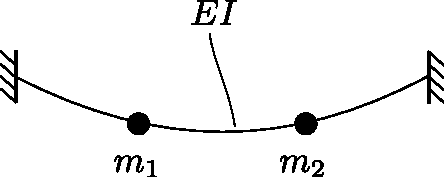
\includegraphics[height=0.14\textwidth]{Bilder/05Biegeschwinger.pdf}}
	\hspace{1.5cm}
	\subfloat[Torsionsschwingerkette]{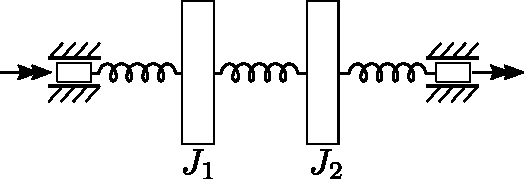
\includegraphics[height=0.15\textwidth]{Bilder/05Torsionsschwingerkette.pdf}}\\[5mm]
	\subfloat[Punktmasse]{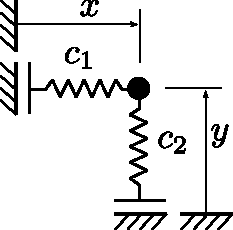
\includegraphics[height=0.17\textwidth]{Bilder/05EbeneSchwingung.pdf}}
	\hspace{2cm}
	\subfloat[Nickschwingungen im Fahrzeug]{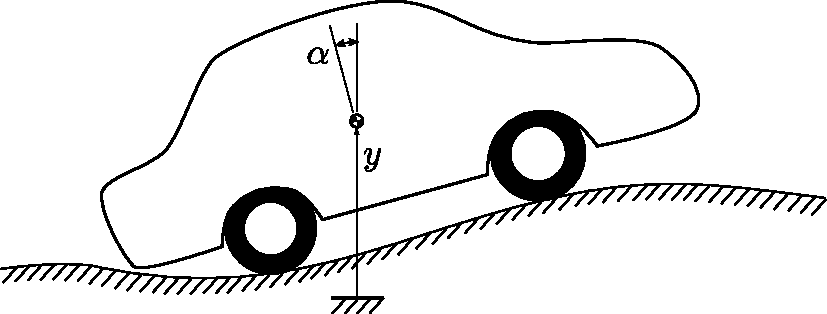
\includegraphics[height=0.23\textwidth]{Bilder/05Nickschwingungen.pdf}}
	\caption{2-Freiheitsgrad-Systeme}
	\label{Abb:2DoFSchwinger}
\end{figure}\\
Im folgenden Abschnitt wird das Ersatzmodell f�r die Vertikalschwingung einer Maschine auf einem Fundament behandelt. Hierbei ist die Maschine durch eine viskoelastische Verbindung auf einem Schwingfundament befestigt.  
\section{Bewegungsgleichung}
Die weiteren Untersuchungen von Zwei-Freiheitsgrad-Systemen werden im Folgenden anhand der Maschine auf Fundament durchgef�hrt. Zun�chst wird der Aufbau und der Freischnitt nach d'Alembert dargestellt: 
\begin{figure}[h]
	\centering
	\subfloat[]{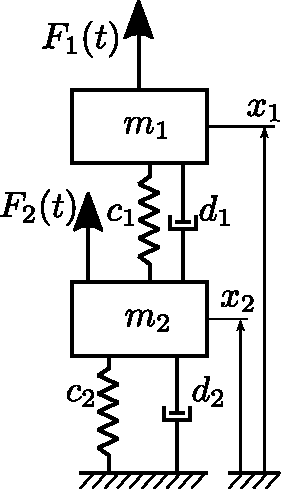
\includegraphics[height=0.38\textwidth]{Bilder/05ZweiMassenSchwinger.pdf}}\hspace{2cm}
	\subfloat[]{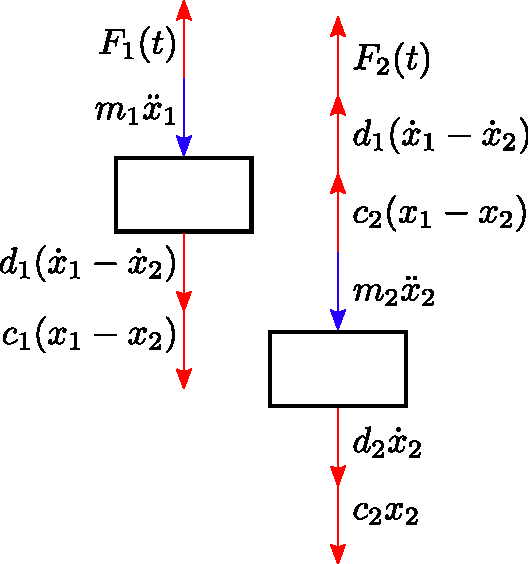
\includegraphics[height=0.41\textwidth]{Bilder/05ZMSdAlembert.pdf}}
	\caption{Schwingungssystem und Freischnitt im Sinne d'Alemberts}
\end{figure}\\
Die Bewegungsgleichung des dargestellten Systems lautet 
\begin{align}
	m_1 \ddot x_1 + d_1 (\dot x_1 - \dot x_2)+ c_1( x_1 - x_2)& = F_1(t) \\
	m_2 \ddot x_2 +d_2 \dot x_2 + d_1 (\dot x_2 - \dot x_1)+ c_2 x_2 +c_1( x_2 - x_1)& = F_2(t)
\end{align}
Diese Gleichungen lauten in Matrix-Vektor-Schreibweise
\begin{align}
\underbrace{
\left[\begin{array}{cc} 
m_1 & 0 \\ 0 & m_2 \\ 
\end{array}\right]}_{M}
\underbrace{\left[\begin{array}{c} 
\ddot x_1  \\ \ddot x_2\\ 
\end{array}\right]}_{\ddot{\vec {x}}}
&+
\underbrace{
\left[\begin{array}{cc} 
d_1 & -d_1 \\ -d_1 & d_1 +d_2 \\ 
\end{array}\right]}_{D}
\underbrace{
\left[\begin{array}{c} 
\dot x_1  \\ \dot x_2\\ 
\end{array}\right]}_{\dot {\vec {x}}}
+ 
\underbrace{
\left[\begin{array}{cc} 
c_1 & -c_1 \\ -c_1 & c_1 + c_2 \\ 
\end{array}\right]}_{K}
\underbrace{
\left[\begin{array}{c} 
x_1  \\ x_2\\ 
\end{array}\right]}_{{\vec {x}}}\nonumber \\
&= 
\underbrace{
\left[\begin{array}{c} 
F_1  \\ F_2\\ 
\end{array}\right]}_{{\vec {F}}}
\end{align}
Hier bei bezeichnet $M$ die Massenmatrix, $D$ die D�mpfungsmatrix, $K$ die Steifigkeitsmatrix, ${\vec {x}}$ den Vektor der Positionen und ${\vec {F}}$ den Vektor der Kraftanregung. Man spricht bei
\begin{align}
	M \ddot{\vec {x}} + D \dot{\vec {x}} + K{\vec {x}} ={\vec {F}}
\end{align}
von einem linearen, gekoppelten, inhomogenen System von Differentialgleichungen von zwei Freiheitsgraden mit konstanten Koeffizienten. 
\section{Unged�mpfte Schwingungen}
Bereits im Kapitel 3 dieser Vorlesung wurden freie und erzwungene Schwingungen von Einfreiheitsgradschwingern behandelt. Die Vorgehensweise ist bei Mehrfreiheitsgradsystemen grunds�tzlich identisch -- es ergeben sich allerdings ein paar Besonderheiten, auf die hier eingegangen werden soll. Es wird zun�chst das unged�mpfte System 
\begin{align}
	M \ddot{\vec {x}} + K{\vec {x}} ={\vec {F}} = \left[\begin{array}{c}
		F_1 \\F_2
	\end{array}\right]\cos(\Omega t)
\end{align}
betrachtet, welches die nun vektorwertige Gesamtl�sung $\vec{x}(t) = \vec{x}_h(t)+\vec{x}_p(t)$ (homogene und partikul�re L�sung) besitzt. Zur Berechnung der homogenen L�sung $\vec{x}_h(t)$ wird zun�chst das System 
\begin{align}
M \ddot{\vec {x}} + K{\vec {x}} = {\vec {0}}
\end{align}
betrachtet und mithilfe eines Exponentialansatz 
\begin{align}
{\vec {x}_h} = {\vec {r}}e^{\lambda t} = \left[\begin{array}{c} 
r_1  \\ r_2\\ 
\end{array}\right]e^{\lambda t}
\end{align}
gel�st. Hierbei ist $\vec r$ der \emph{Eigenvektor} und $\lambda$ der zu bestimmende Eigenwert. Ableiten und Einsetzen in die Bewegungsdifferentialgleichung liefert 
\begin{align}
\dot{\vec {x}}_h &= \lambda {\vec {r}} e^{\lambda t} \\
\ddot{\vec {x}}_h &= \lambda^2{\vec {r}} e^{\lambda t}\\
(M \lambda^2 + K ){\vec {r}} e^{\lambda t} & = {\vec {0}}
\end{align}
Die algebraische Gleichung 
\begin{align}
(M \lambda^2 + K ){\vec {r}} & = {\vec {0}}
\label{eq:EWP}
\end{align}
hei�t \emph{Eigenwertproblem}. Die Bilanz der Anzahl Gleichungen und Unbekannter zeigt: Es gibt zwei Gleichungen zur Bestimmung der zwei Komponenten von $\vec r$ sowie den Eigenwert $\lambda$ -- das Gleichungssystem ist also unterbestimmt. Diese Situation kennen wir schon vom 1-Freiheitsgrad-System, wo die Amplitude der Koeffizienten des Exponentialansatzes erst durch Zusatzbedingungen (Anpassung an die Anfangsbedingungen) gefunden werden kann. \\
Zur L�sung wird die folgende Betrachtung herangezogen:  Wenn die Matrix $(M \lambda^2 + K )$ invertierbar ist, dann folgt direkt die triviale L�sung ${\vec {r}}={\vec {0}}$, also ${\vec {x}}_h={\vec {0}}$. Um allgemeine nicht-triviale L�sungen zuzulassen, darf $(M \lambda^2 + K )$ also nicht invertierbar sein. Daher muss die Determinante dieser Matrix verschwinden: 
\begin{align}
	\det (M \lambda^2 + K ) = 0
\end{align}
Diese Gleichung ist im Fall von 2-Freihetsgrad-Systemen mit $M\in \mathbb{R}^{2\times2}$, $K\in \mathbb{R}^{2\times2}$ ein Polynom 4. Grades in $\lambda$. Die Eigenwerte $\lambda_i$, $i\in \{1,2,3,4\}$ treten in konjugiert komplexen Paaren auf: 
\begin{align}
&\lambda_{1/2}=\pm i \omega_1& &\lambda_{3/4}=\pm i \omega_3&
\end{align}
Zur Bestimmung der Eigenvektoren werden die Eigenwerte in das Eigenwertproblem \ref{eq:EWP} eingesetzt: 
\begin{align}
&\lambda_{i}:&  &( M \lambda_i^2 + K )\vec{r}_{i} = 0& &i\in\{1,2,3,4\}&
\label{eq:EV}
\end{align}
Wegen der Singularit�t der Matrix $( M \lambda_i^2 + K )$ sind die Zeilen des Gleichungssystems \ref{eq:EV} linear abh�ngig. Der L�sungsvektor $\vec{r}_i$ kann bis auf eine freie Konstante berechnet werden. Es verbleiben also insgesamt 4 Konstanten zur Bestimmung der freien Schwingung $\vec{x}_h(t)$, die durch die Anfangsbedingungen gew�hlt werden. \\
Die Quadrate der Eigenwerte sind $\lambda_{1/2}^2 = -\omega_{1}^2$,  $\lambda_{3/4}^2 =-\omega_3^2$. Daher sind die Bestimmungsgleichungen f�r $\vec{r}_1$ und $\vec{r}_2$ identisch, ebenso f�r $\vec{r}_3$ und $\vec{r}_4$; es folgt $\vec{r}_1 = \vec{r}_2$ und $\vec{r}_3 = \vec{r}_4$. Die homogene L�sung lautet schlussendlich 
\begin{align}
&\vec{x}_h(t) = \tilde C_1 \vec{r}_{1/2} e^{i\omega_{1} t} + \tilde C_2 \vec{r}_{1/2} e^{-i\omega_{1} t} + \tilde C_3 \vec{r}_{3/4} e^{i\omega_{3} t} + \tilde C_4 \vec{r}_{3/4} e^{-i\omega_{3} t}
\end{align}
oder in reeller Darstellung 
\begin{align}
&\vec{x}_h(t) = C_1 \vec{r}_1 \sin (\omega_1 t) + C_2 \vec{r}_1 \cos(\omega_1 t) + C_3 \vec{r}_3 \sin (\omega_3 t) + C_4 \vec{r}_3 \cos(\omega_3 t) 
\end{align}
Die Massenmatrix $M$ und die Steifigkeitsmatrix $K$ sind positiv definit, sprich, $\det(M)>0$ und $\det(K)>0$. Dann sind die Eigenwerte stets imagin�r und die Eigenvektoren reellwertig. \\
F�r die partikul�re L�sung $x_p(t)$ des zwangserregten Systems wird der vektorwertige Ansatz vom Typ der rechten Seite eingesetzt: 
\begin{align}
	&\vec{x}_p = \vec{p} \cos(\Omega t)+\vec{q} \sin(\Omega t)&
	&\ddot{\vec{x}}_p = -\Omega^2\vec{p} \cos(\Omega t)-\Omega^2\vec{q} \sin(\Omega t)&
\end{align}
Hierbei sind $\vec{p}$ und $\vec{q}$ die noch zu bestimmenden Amplituden. Einsetzen liefert 
\begin{align}
	&-\Omega^2 M \vec{p} \cos(\Omega t)-\Omega^2 M \vec{q} \sin(\Omega t)
	+ K \vec{p} \cos(\Omega t)+K \vec{q} \sin(\Omega t) = \vec{F}\cos(\Omega t)
\end{align}
Der Koeffizientenvergleich ergibt zwei Gleichungen 
\begin{align}
	&\cos(\Omega t):& &-\Omega^2 M \vec{p} + K \vec{p} = \vec{F} &\\
	&\sin(\Omega t):&&-\Omega^2 M \vec{q} +K \vec{q}  = \vec{0}&
\end{align}
Es folgen die L�sungen 
\begin{align}
	&\vec{p}=(K-\Omega^2 M)^{-1}\vec{F}& 
	&\vec{q} = \vec{0}&
	\label{eq:pqpar}
\end{align}
Als Gesamtl�sung ergibt sich durch Superposition 
\begin{align}
	\vec{x}(t) =& \vec{x}_h(t)+\vec{x}_p(t)\\
	=& C_1 \vec{r}_1 \sin (\omega_1 t) + C_2 \vec{r}_1 \cos(\omega_1 t) + C_3 \vec{r}_3 \sin (\omega_3 t) + C_4 \vec{r}_3 \cos(\omega_3 t)\nonumber\\
	&+ (K-\Omega^2 M)^{-1}\vec{F}\cos(\Omega t)\nonumber
\end{align}
Die freien Konstanten k�nnen jetzt mithilfe der Anfangsbedingungen bestimmt werden. Hierzu lauten die vier Gleichungen 
\begin{align}
	\vec{x}_0 = \vec{x}(t=0) =& C_2 \vec{r}_1 +C_4 \vec{r}_3 + (K-\Omega^2 M)^{-1}\vec{F}\\
	\vec{v}_0 = \dot{\vec{x}}(t=0) =& \omega_1 C_1 \vec{r}_1 +\omega_3 C_3 \vec{r}_3 - \Omega (K-\Omega^2 M)^{-1}\vec{F}	
\end{align}
welche die Gleichungssysteme 
\begin{align}
	\vec{x}_0 - (K-\Omega^2 M)^{-1}\vec{F} &= \left[\vec{r}_1, \vec{r}_3\right]\left[\begin{array}{c}
		C_1\\C_3
	\end{array}\right] \\
	\vec{v}_0 + \Omega (K-\Omega^2 M)^{-1}\vec{F} &= \left[\omega_1 \vec{r}_1,\omega_3 \vec{r}_3\right] \left[\begin{array}{c}
		C_2\\C_4
	\end{array}\right]	
\end{align}
ergeben. 
\begin{theo}[Ausz�ge aus der linearen Algebra]{theo:LinAlg}
	Transposition eines Vektors: 
	\begin{align*}
	x^T = \left[
	\begin{array}{c}
		x_{1} \\ x_{2} 
	\end{array}\right]^T
	=\left[
	\begin{array}{cc}
	x_{1} & x_{2} 
\end{array}\right]
\end{align*}
	Transposition einer Matrix: 
	\begin{align*}
		A^T = \left[
		\begin{array}{cc}
			A_{11} & A_{12} \\
			A_{21} & A_{22}
		\end{array}\right]^T
  	= \left[
	\begin{array}{cc}
		A_{11} & A_{21} \\
		A_{12} & A_{22}
	\end{array}\right]
\end{align*}
	Skalarprodukt: 
	\begin{align*}
		\vec{x}\cdot \vec{y}=
		\left[
		\begin{array}{c}
			x_{1} \\
			x_{2}
		\end{array}\right]\cdot
		\left[
		\begin{array}{c}
			y_{1} \\
			y_{2}
		\end{array}\right]
		=
		x_1 y_1 + x_2 y_2
	\end{align*}	
	oder in alternativer Schreibweise 
	\begin{align*}
		\vec{x}\cdot \vec{y}= \vec{x}^T \vec{y} =
		\left[
		\begin{array}{cc}
			x_{1} &	x_{2}
		\end{array}\right] \left[
		\begin{array}{c}
			y_{1} \\
			y_{2}
		\end{array}\right]
		=
		x_1 y_1 + x_2 y_2
	\end{align*}	
	Matrix-Vektor-Produkt: 
	\begin{align*}
		A \vec{x} = \left[
		\begin{array}{cc}
			A_{11} & A_{12} \\
			A_{21} & A_{22}
		\end{array}\right]
		\left[
		\begin{array}{c}
			x_{1} \\
			x_{2}
		\end{array}\right]
		=
		\left[
		\begin{array}{c}
			A_{11}x_{1}+A_{12}x_{2}\\
			A_{21}x_{1}+A_{22}x_{2}
		\end{array}\right]
	\end{align*}	
	Skalarprodukt mit Matrix-Vektor-Produkt: 
	\begin{align*}
		\vec{x}\cdot (A \vec{y}) &= 	\left[
		\begin{array}{c}
			x_{1} \\
			x_{2}
		\end{array}\right]\cdot \left(
		\left[
		\begin{array}{cc}
			A_{11} & A_{12} \\
			A_{21} & A_{22}
		\end{array}\right]
		\left[
		\begin{array}{c}
			y_{1} \\
			y_{2}
		\end{array}\right]\right)
		=
		\left[
		\begin{array}{c}
			x_{1} \\
			x_{2}
		\end{array}\right]\cdot \left[
		\begin{array}{c}
			A_{11}y_{1}+A_{12}y_{2}\\
			A_{21}y_{1}+A_{22}y_{2}
		\end{array}\right]\\
		&= x_1 y_{1} A_{11}+x_1 y_{2} A_{12} + x_2y_{1} A_{21}+x_2y_{2} A_{22}\\
		\vec{y}\cdot (A \vec{x}) &=x_{1}y_1 A_{11}+ x_{1}y_2 A_{21}+x_{2}y_1 A_{12}+x_{2}y_2 A_{22}
	\end{align*}	
	Gem�� der letzten Formel gilt die Vertauschungsrelation
	\begin{align*}
		\vec{x}\cdot (A \vec{y}) = \vec{y}\cdot (A^T \vec{x})
	\end{align*}
	Matrix-Matrix-Produkt: 
	\begin{align*}
		A B & = \left[
		\begin{array}{cc}
			A_{11} & A_{12} \\
			A_{21} & A_{22}
		\end{array}\right]
		\left[
		\begin{array}{cc}
			B_{11} & B_{12} \\
			B_{21} & B_{22}
		\end{array}\right]\\
		& = \left[
		\begin{array}{cc}
			A_{11}B_{11} + A_{12}B_{21} & A_{11}B_{12} + A_{12}B_{22} \\
			A_{21}B_{11} + A_{22}B_{21} & A_{21}B_{12} + A_{22}B_{22} 
		\end{array}\right]
	\end{align*}
	Aus Vektoren zusammengesetzte Matrix: 
	\begin{align*}
		R = \left[\vec{x},\vec{y}\right] 
		= \left[
		\begin{array}{cc}
			x_{1} & y_{1} \\
			x_{2} & y_{2}
		\end{array}\right]
	\end{align*}
\end{theo}
\begin{beispiel}[Unged�mpfter 2-Massen-Schwinger]{beispiel:Unged2MS}
Im betrachteten System zur Berechnung von Eigenwerten und Eigenvektoren sei $m_1=m$, $m_2=8m$,  $c_1=c$, $c_2=5c$, $d_1=d_2=0$. Die Bewegungsgleichung lautet 
\begin{align}
\underbrace{
	\left[\begin{array}{cc} 
	m & 0 \\ 0 & 8m \\ 
	\end{array}\right]}_{M}
\underbrace{\left[\begin{array}{c} 
	\ddot x_1  \\ \ddot x_2\\ 
	\end{array}\right]}_{\ddot{ \vec{x}}}
+
\underbrace{
	\left[\begin{array}{cc} 
	c & -c \\ -c & 6c \\ 
	\end{array}\right]}_{K}
\underbrace{
	\left[\begin{array}{c} 
	x_1  \\ x_2\\ 
	\end{array}\right]}_{\vec{x}}
= 
	\left[\begin{array}{c} 
	F_1  \\ 0\\ 
	\end{array}\right]\cos(\Omega t)
\end{align}
Mit dem Expontialansatz f�r die homogene L�sung $\vec{x}_h = \vec{r} e^{\lambda t}$ folgt $\ddot{\vec{x}}_h = \lambda^2 \vec{r} e^{\lambda t}$ und 
\begin{align}
(M\lambda^2 + K) \vec{r} e^{\lambda t}= \vec{0}
\label{eq:BEV}
\end{align}
Aus der Forderung nach der Existenz der nicht-trivialen L�sung $\vec{r}\neq \vec{0}$ folgt das charakteristische Polynom 
\begin{align}
	0 &= \det(M\lambda^2 + K) = \left|
	\left[\begin{array}{cc} 
	m\lambda^2+ c & -c \\ -c & 8m\lambda^2 + 6c \\ 
	\end{array}\right]
	\right| \\
	&= 8 m^2\lambda^4 + 14cm\lambda^2 + 5c^2 
\end{align}
Die Eigenwerte sind
\begin{align}
&\lambda_{1/2} = \pm i\sqrt{\frac{c}{2m}}&
&\lambda_{3/4} = \pm i\sqrt{\frac{5c}{4m}}&
\end{align}
Wird $\lambda_{1/2}$ in Gl. (5.19) eingesetzt, dann ist 
\begin{align}
0 &= (M\lambda_{1/2}^2 + K) \vec{r}_{1/2} = 
\left[\begin{array}{cc} 
m\lambda_{1/2}^2+ c & -c \\ -c & 8m\lambda_{1/2}^2 + 6c \\ 
\end{array}\right]
	\left[\begin{array}{c} 
r_1  \\ r_2\\ 
\end{array}\right]_{1/2}\\
&= \left[\begin{array}{cc} 
\frac{1}{2}c  & -c \\ 
-c  & 2c \\ 
\end{array}\right]
\left[\begin{array}{c} 
r_1  \\ r_2\\ 
\end{array}\right]_{1/2}
\end{align}
Mit $\vec{r}_{1/2}$ dem zum Eigenwertpaar $\lambda_{1/2}$ geh�rigen Eigenvektorpaar. Die Eigenvektoren $\vec{r}_{1}$ und $\vec{r}_{2}$ sind identisch. Die zwei Zeilen von Gl.(5.26) sind linear abh�ngig. Das Gleichungssystem hat unendlich viele L�sungen -- die L�sung kann also nur bis auf eine Konstante bestimmt werden. Setze $r_1 = z$, dann folgt
\begin{align}
\vec{r}_{1/2} = 
\left[\begin{array}{c} 
z \\ \frac{1}{2}z\\ 
\end{array}\right]
\end{align}
Die zus�tzliche Forderung nach $|\vec{r}_{1/2}|=\sqrt{5}z \overset{!}{=}1$ f�hrt zum \emph{normierten Eigenvektor}
\begin{align}
&\vec{r}_{1/2} = \frac{1}{\sqrt{5}}
\left[\begin{array}{c} 
2  \\ 1\\ 
\end{array}\right]&
&|\vec{r}_{1/2}|=1&
\end{align}
Beim Eigenwertpaar $\lambda_{3/4}$ ergibt sich 
\begin{align}
0 = (M\lambda_{3/4}^2 + K) \vec{r}_{3/4} 
= \left[\begin{array}{cc} 
\frac{1}{4}c & -c\\ 
-c  & 4c\\ 
\end{array}\right]
\left[\begin{array}{c} 
r_1  \\ r_2\\ 
\end{array}\right]_{3/4}
\end{align}
und der zugeh�rige normierte Eigenvektor ist 
\begin{align}
&\vec{r}_{3/4} = \frac{1}{\sqrt{17}}
\left[\begin{array}{c} 
4  \\ -1\\ 
\end{array}\right]&
\end{align}
Die homogene L�sung ist in reeller Darstellung 
\begin{align}
\vec{x}_h(t) = C_1 \vec{r}_{1/2} \sin (\omega_1 t) + C_2 \vec{r}_{1/2} \cos(\omega_1 t) + C_3 \vec{r}_{3/4} \sin (\omega_3 t) + C_4 \vec{r}_{3/4} \cos(\omega_3 t) 
\end{align}
Die Eigenvektoren $\vec{r}_{1/2}$ und $\vec{r}_{3/4}$ kennzeichnen die Eigenschwingungsformen: 
\begin{itemize}
	\item 1. Eigenschwingungsform bei $\omega_1 = \sqrt{\frac{c}{2m}}$. Die Bewegung beider Massen ist gleichphasig, da die Vorzeichen der Komponenten von $\vec{r}_{1/2}$ gleich sind
	\item 2. Eigenschwingungsform bei $\omega_3 = \sqrt{\frac{5c}{4m}}$. Die Bewegung beider Massen ist gegenphasig, da die Vorzeichen der Komponenten von $\vec{r}_{3/4}$ verschieden sind
\end{itemize}
Die partikul�re L�sung folgt direkt nach Gl. (5.22)
\begin{align}
	\vec{x}_p(t) & = (K-\Omega^2 M)^{-1}\vec{F} = 
	\left[\begin{array}{cc} 
		c-m\Omega^2+  & -c \\ -c & 6c-8m\Omega^2 \\ 
	\end{array}
	\right]^{-1}\left[\begin{array}{c}
		F_1\\ 0
	\end{array}\right]\cos(\Omega t)\\
& = \frac{F_1}{8 m^2\Omega^4 - 14cm\Omega^2 + 5c^2 }\left[\begin{array}{c}
	6 c-8m\Omega^2\\ c
\end{array}\right]\cos(\Omega t)
\end{align}
Die Konstanten $C_i$, $i\in \{1,...,4\}$ werden durch Anpassung an die Anfangsbedingungen zu 
\begin{align}
\left[
\begin{array}{c}
C_1 \\ C_3
\end{array}\right] &= 
\left[
\begin{array}{cc}
\frac{2\sqrt{5}}{3} & \frac{\sqrt{5}}{6} \\ 
\frac{\sqrt{17}}{3}&-\frac{\sqrt{17}}{6}
\end{array}\right]
\left[\vec x_0-\vec{p}\right] \\
&= \left[
\begin{array}{c}
\frac{\sqrt{5}}{6}(4 x_{01}+x_{02}) \\ \frac{\sqrt{17}}{6}(2 x_{01}-x_{02})
\end{array}\right]\\
&-\frac{F_1}{8 m^2\Omega^4 - 14cm\Omega^2 + 5c^2 }\left[\begin{array}{c}
	\frac{2\sqrt{5}}{3}(6 c-8m\Omega^2)+\frac{\sqrt{5}}{6} c\\
	\frac{\sqrt{17}}{3}(6 c-8m\Omega^2)+\frac{\sqrt{17}}{6} c	
\end{array}\right]\nonumber
\end{align}
\begin{align}
\left[
\begin{array}{c}
C_2 \\ C_4
\end{array}\right] &= 
\left[
\begin{array}{cc}
\frac{2\sqrt{5}}{3\omega_1} & \frac{\sqrt{5}}{6\omega_1} \\ 
\frac{\sqrt{17}}{3\omega_3} &-\frac{\sqrt{17}}{6\omega_3} \\ 
\end{array}\right]
\left[
\begin{array}{c}
	\vec{v}_0+\Omega \vec{p}
\end{array}\right] \\
&= \left[
\begin{array}{c}
\frac{\sqrt{5}}{6\omega_1}(4 v_{01}+v_{02}) \\ \frac{\sqrt{17}}{6\omega_3}(2 v_{01}-v_{02})
\end{array}\right] \\
&+\frac{\Omega F_1}{8 m^2\Omega^4 - 14cm\Omega^2 + 5c^2 }\left[\begin{array}{c}
	\frac{2\sqrt{5}}{3\omega_1}(6 c-8m\Omega^2)+\frac{\sqrt{5}}{6\omega_1} c\\
	\frac{\sqrt{17}}{3\omega_3}(6 c-8m\Omega^2)+\frac{\sqrt{17}}{6\omega_3} c	
\end{array}\right]\nonumber
\end{align}
\end{beispiel}
\section{Modale Entkopplung}
Die beiden Eigenwertpaare $(\omega_i,\vec{r}_i)$ und $(\omega_j,\vec{r}_j)$ erf�llen jeweils das Eigenwertproblem ${(-\omega_i^2 M +K)\vec{r}_i=\vec{0}}$ bzw. ${(-\omega_j^2 M +K)\vec{r}_j=\vec{0}}$. Die Multiplikation dieser Gleichungen mit dem jeweils anderen Eigenvektor liefert zwei skalare Gleichungen 
\begin{align}
	&-\omega_i^2 \vec{r}_j\cdot (M\vec{r}_i) + \vec{r}_j\cdot (K \vec{r}_i)=\vec{r}_j\cdot \vec{0} = 0\label{eq:EWPij1}\\
	&-\omega_j^2 \vec{r}_i\cdot (M\vec{r}_j) + \vec{r}_i\cdot (K \vec{r}_j)=\vec{r}_i\cdot \vec{0} = 0
\label{eq:EWPij2}
\end{align}
Ferner ist, gemeinsam mit der Vertauschungsrelation aus (Mathematik 5.1),
\begin{align}
&-\omega_i^2 \vec{r}_j\cdot (M\vec{r}_i) + \vec{r}_j\cdot (K \vec{r}_i)= 
-\omega_i^2 \vec{r}_i\cdot (M^T\vec{r}_j) + \vec{r}_i\cdot (K^T \vec{r}_j)
\end{align}
Sowohl Massen- als auch Steifigkeitsmatrix sind symmetrisch, weshalb $M^T=M$ und $K^T=K$.  Einsetzen in Gl. \ref{eq:EWPij1} und Subtraktion mit Gl. \ref{eq:EWPij2} f�hrt auf 
\begin{align}
&-(\omega_j^2 - \omega_i^2 )\vec{r}_i\cdot (M\vec{r}_j) = 0 
\end{align}
F�r einfache Eigenwerte gilt $\omega_i\neq\omega_j$ $(i\neq j)$; dann sind die Eigenvektoren \emph{bez�glich der Massenmatrix orthogonal}: 
\begin{align}
&\vec{r}_i\cdot (M\vec{r}_j) = 0 
\end{align}
Aus Gl. \ref{eq:EWPij2} folgt dann direkt die Orthogonalit�t bez�glich der Steifigkeitsmatrix
\begin{align}
&\vec{r}_i\cdot (K\vec{r}_j) = 0 
\end{align}
F�r $i=j$ ist 
\begin{align}
	&-\omega_i^2 \vec{r}_i\cdot (M\vec{r}_i) + \vec{r}_i\cdot (K \vec{r}_i)= 0
\end{align}
und damit der \emph{Rayleigh}-Quotient 
\begin{align}
&\omega_i^2  = \frac{\vec{r}_i\cdot (K \vec{r}_i)}{\vec{r}_i\cdot (M\vec{r}_i)}
\end{align}
definiert. Wenn die Eigenwerte massenbezogen normiert werden, d.h. ${\vec{r}_i\cdot (M\vec{r}_i)=1}$, dann vereinfacht sich der Rayleigh-Quotient zu ${\omega_i^2  = \vec{r}_i\cdot (K \vec{r}_i)}$. Ferner wird die \emph{Modalmatrix} definiert durch die Matrix der linear unabh�ngigen Eigenvektoren
\begin{align}
R  = [\vec{r}_1, \vec{r}_3]
\end{align}
Da die Eigenvektoren den Zustandsraum vollst�ndig aufspannen, kann der Zustandsvektor auch wie folgt dargestellt werden: 
\begin{align}
\vec{x} = \left[
\begin{array}{c}
x_1\\x_2
\end{array}
\right]
 = 
z_1 \vec{r}_1 + z_3 \vec{r}_3 = 
[\vec{r}_1,\vec{r}_3]\left[
\begin{array}{c}
z_1\\z_3
\end{array}
\right] = 
R  \vec{z}
\end{align}
und folglich ist das zwangserregte System
\begin{align}
	\vec{F} & = M\ddot{\vec{x}} + K \vec{x} 
	= M \left([\vec{r}_1,\vec{r}_3]\left[
	\begin{array}{c}
	\ddot z_1\\\ddot z_3
	\end{array}
	\right]\right) + K \left([\vec{r}_1,\vec{r}_3]\left[
	\begin{array}{c}
	z_1\\z_3
	\end{array}
	\right]\right)\\
	&=  M R  \ddot{ \vec{z}} + K R  \vec{z}
\end{align}
Linksmultiplikation mit $R^T$ f�hrt zu 
\begin{align}
R^T\vec{F} & = 
R^T M R  \ddot{ \vec{z}} + R^T K R  \vec{z}\\ 
&= 	\left[
\begin{array}{c}
\vec{r}_1^T\\\vec{r}_3^T
\end{array}\right]
M [\vec{r}_1,\vec{r}_3]\left[
\begin{array}{c}
\ddot z_1\\\ddot z_3
\end{array}
\right]
+ \left[
\begin{array}{c}
\vec{r}_1^T\\\vec{r}_3^T
\end{array}\right] K [\vec{r}_1,\vec{r}_3]\left[
\begin{array}{c}
z_1\\z_3
\end{array}
\right]
\end{align}
\begin{align}
& =  	\left[
\begin{array}{cc}
\vec{r}_1^T M \vec{r}_1& \vec{r}_1^T M \vec{r}_3\\
\vec{r}_3^T M \vec{r}_1& \vec{r}_3^T M \vec{r}_3
\end{array}\right]
\left[
\begin{array}{c}
\ddot z_1\\\ddot z_3
\end{array}
\right]+
\left[\begin{array}{cc}
\vec{r}_1^T K \vec{r}_1& \vec{r}_1^T K \vec{r}_3\\
\vec{r}_3^T K \vec{r}_1& \vec{r}_3^T K \vec{r}_3
\end{array}\right]
\left[\begin{array}{c}
z_1\\z_3
\end{array}
\right]0
\end{align}
Bzw.
\begin{align}
\left[
\begin{array}{c}
	\vec{r}_1\cdot \vec{F}\\\vec{r}_3\cdot \vec{F}
\end{array}
\right]&=  	\left[
\begin{array}{cc}
1& 0\\
0& 1
\end{array}\right]
\left[
\begin{array}{c}
\ddot z_1\\\ddot z_3
\end{array}
\right]+
\left[\begin{array}{cc}
\omega_1^2& 0\\
0& \omega_3^2
\end{array}\right]
\left[\begin{array}{c}
z_1\\z_3
\end{array}
\right]
\end{align}
Es liegen also zwei entkoppelte Einzeldifferentialgleichungen vor: 
\begin{align}
	& \ddot z_1+\omega_1^2 z_1 = \vec{r}_1\cdot \vec{F} &
	& \ddot z_3+\omega_3^2 z_3 = \vec{r}_3\cdot \vec{F} & 
\end{align}
Modale Entkopplung des Differentialgleichungssystems setzt die Kenntnis der Eigenvektoren voraus. Der Vorteil der modalen Entkopplung ist, dass die Gleichungen unabh�ngig voneinander gel�st werden k�nnen. Dies ist insbesondere bei erzwungenen Schwingungen vorteilhaft. 
\begin{beispiel}[Modale Entopplung]{beispiel:Modalmatrix}
Es wird das unged�mpfte System 
\begin{align}
	\left[\begin{array}{cc} 
		8m & 0 \\ 0 & m \\ 
	\end{array}\right]
	\left[\begin{array}{c} 
		\ddot x_1  \\ \ddot x_2\\ 
	\end{array}\right]
	+
	\left[\begin{array}{cc} 
		6c & -c \\ -c & c \\ 
	\end{array}\right]
	\left[\begin{array}{c} 
		x_1  \\ x_2\\ 
	\end{array}\right]
	= 
	\left[\begin{array}{c} 
		F_0\cos(\Omega t)  \\ 0\\ 
	\end{array}\right]
\end{align}
betrachtet. Die Eigenwertpaare sind vor Normierung 
\begin{align}
	& \omega_1 = \sqrt{\frac{c}{2m}}& 
	& \vec{r}_1 = C_1 \left[\begin{array}{c}
		1\\2
	\end{array}\right]& \\
	& \omega_3 = \sqrt{\frac{5c}{4m}}& 
	& \vec{r}_3 = C_3 \left[\begin{array}{c}
		1\\-4
	\end{array}\right]&
\end{align} 
Die Normierung bzgl. der Massenmatrix liefert die freien Konstanten
\begin{align}
	&\vec{r}_1\cdot (M\vec{r}_1) = 12 C_1^2 m \overset{!}{=} 1&
	&\rightarrow&
	&C_1 = \frac{1}{2\sqrt{3m}}&  \\
	&\vec{r}_3\cdot (M\vec{r}_3) = 24 C_3^2 m \overset{!}{=} 1&
	&\rightarrow&
	&C_3 = \frac{1}{2\sqrt{6m}}&  
\end{align}
Die Modalmatrix ist 
\begin{align}
	R = [\vec{r}_1, \vec{r}_3] = 
	\left[\begin{array}{cc}
		\frac{1}{2\sqrt{3m}}& \frac{1}{2\sqrt{6m}}\\
		\frac{1}{\sqrt{3m}}& -\frac{2}{\sqrt{6m}}
	\end{array}\right]
\end{align}
Die modal entkoppelte Massen- und Steifigkeitsmatrix lauten 
\begin{align}
	R^T M R  &= 
	\left[\begin{array}{cc}
		\frac{1}{2\sqrt{3m}}& \frac{1}{\sqrt{3m}}\\
		\frac{1}{2\sqrt{6m}}& -\frac{2}{\sqrt{6m}}
	\end{array}\right]
	\left[\begin{array}{cc}
		8m& 0\\
		0& m
	\end{array}\right]
	\left[\begin{array}{cc}
		\frac{1}{2\sqrt{3m}}& \frac{1}{2\sqrt{6m}}\\
		\frac{1}{\sqrt{3m}}& -\frac{2}{\sqrt{6m}}
	\end{array}\right]\\
	& = \left[\begin{array}{cc}
		1& 0\\
		0& 1
	\end{array}\right]
\end{align}
ferner 
\begin{align}
	R^T K R  &= 
	\left[\begin{array}{cc}
		\frac{1}{2\sqrt{3m}}& \frac{1}{\sqrt{3m}}\\
		\frac{1}{2\sqrt{6m}}& -\frac{2}{\sqrt{6m}}
	\end{array}\right]
	\left[\begin{array}{cc}
		6c& -c\\
		-c& c
	\end{array}\right]
	\left[\begin{array}{cc}
		\frac{1}{2\sqrt{3m}}& \frac{1}{2\sqrt{6m}}\\
		\frac{1}{\sqrt{3m}}& -\frac{2}{\sqrt{6m}}
	\end{array}\right]\\
	& = \left[\begin{array}{cc}
		\frac{c}{2m}& 0\\
		0& \frac{5c}{4m}
	\end{array}\right]
\end{align}
und 
\begin{align}
	R^T F  &= 
	\left[\begin{array}{cc}
		\frac{1}{2\sqrt{3m}}& \frac{1}{\sqrt{3m}}\\
		\frac{1}{2\sqrt{6m}}& -\frac{2}{\sqrt{6m}}
	\end{array}\right]
	\left[\begin{array}{c}
		F_0\cos(\Omega t)\\
		0
	\end{array}\right]
	= 
	\left[\begin{array}{c}
		\frac{F_0\cos(\Omega t)}{2\sqrt{3m}} \\
		\frac{F_0\cos(\Omega t)}{2\sqrt{6m}}
	\end{array}\right]
\end{align}
Das gekoppelte Differentialgleichungssystem $M\ddot{ \vec{x}} + K \vec{x} = \vec{F}$ wurde also transformiert in zwei voneinander entkoppelte Differentialgleichungen $\ddot z_1 + \omega_1^2 z_1 = F_0\cos(\Omega t)/(2\sqrt{3m})$ und $\ddot z_3 + \omega_3^2 z_3=F_0\cos(\Omega t)/(2\sqrt{6m}) $, die unabh�ngig voneinander gel�st werden k�nnen. \end{beispiel}
\section{Systeme mit modaler D�mpfung}
Im Fall von D�mpfung und ohne �u�ere Anregung lautet die Systembeschreibung 
\begin{align}
M \ddot{\vec {x}} + D \dot{\vec {x}} + K{\vec {x}} ={\vec {0}}
\end{align}
Unter \emph{modaler D�mpfung} versteht man eine spezielle Zusammensetzung der D�mpfungsmatrix der Form 
\begin{align}
D = \alpha M + \beta K
\end{align}
also massen- und steifigkeitsproportionale Anteile der D�mpfung mit Parametern $\alpha$ und $\beta$. Die homogene L�sung des ged�mpften Systems wird mithilfe des Exponentialansatzes $\vec{x}=\vec{r}e^{\lambda t}$ nach 
\begin{align}
&\left(\lambda^2 M + (\alpha M + \beta K)\lambda + K \right)\vec{r}e^{\lambda t}=\vec{0}\\
&\left[\left(\lambda^2 + \lambda \alpha \right)M  + \left(\lambda \beta + 1 \right) K \right]\vec{r}e^{\lambda t}=\vec{0}\\
&\left[\underbrace{\frac{\lambda^2 + \lambda \alpha }{\lambda \beta + 1 }}_{\mu_g} M +  K \right]\vec{r}e^{\lambda t}=\vec{0}\\
\end{align}
berechnet. Wie im unged�mpften Fall wird hier $\vec{r}\neq\vec{0}$ gefordert, weshalb die Bestimmung der Eigenwerte aus 
\begin{align}
	\det(\mu_g M + K)=0
\end{align}
folgt. Man stelle fest, dass es sich hier um dieselbe Struktur wie im zugeh�rigen unged�mpften Schwingungssystem $M\ddot{\vec{x}} + K\vec{x}=\vec{0}$ handelt, welche mit dem unged�mpften Eigenwertproblem $(\lambda_u^2M+K)\vec{r}_u=\vec{0}$ verbunden ist. Damit ist $\lambda_u^2 = \mu_g$ und $\vec{r} = \vec{r}_u$, sprich: \\[5mm]
\begin{lem}[Eigenwerte und -vektoren bei modaler D�mpfung]{lem:ModaleDaempfung}
Die Eigenvektoren im unged�mpften System 
\begin{align}
	M \ddot{\vec {x}} + K{\vec {x}} ={\vec {0}}
\end{align}
und im modal ged�mpften System 
\begin{align}
	M \ddot{\vec {x}} + (\alpha M + \beta K) \dot{\vec {x}} + K{\vec {x}} ={\vec {0}}
\end{align}
sind bei beliebigen $\alpha$, $\beta$ und ansonsten gleichen Parametern identisch. Die ged�mpften und unged�mpften Eigenwerte unterscheiden sich. 
\end{lem}
Die Schlussfolgerung ist, dass unged�mpften Eigenvektoren zur modalen Entkopplung verwendet werden k�nnen: 
\begin{align}
R^T M R &=  	\left[
\begin{array}{cc}
	1& 0\\
	0& 1
\end{array}\right]\\
R^T K R &=  	
\left[\begin{array}{cc}
	\omega_1^2& 0\\
	0& \omega_3^2
\end{array}\right]\\
R^T D R &=\alpha R^T M R + \beta R^T K R = 
\alpha \left[\begin{array}{cc}
1& 0\\
0& 1
\end{array}\right]+ 
\beta \left[\begin{array}{cc}
\omega_1^2& 0\\
0& \omega_3^2
\end{array}\right]
\end{align}
Mit der rechten Seite $R^T \vec{F}$ kann nun folglich das entkoppelte System gel�st werden, um freie und erzwungene Schwingungen zu berechnen. 
\section{Erzwungene Koppelschwingungen und Tilgung}
In diesem Abschnitt wird der unged�mpfte Zwei-Massen-Schwinger mit $F_2(t)=0$ und $F_1(t)=F_0\cos(\Omega t)$ betrachtet. 
\begin{figure}[H]
	\centering
	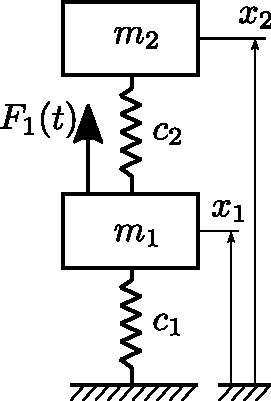
\includegraphics[width=0.2\textwidth]{Bilder/05ErzwungeneKoppelschwingungen.pdf}
	\caption{Zwei-Massen-Schwinger mit �u�erer Anregung}
\end{figure}
Die Bewegungsgleichungen sind in Matrix-Vektor-Schreibweise
\begin{align}
\underbrace{
	\left[\begin{array}{cc} 
	m_1 & 0 \\ 0 & m_2 \\ 
	\end{array}\right]}_{M}
\underbrace{\left[\begin{array}{c} 
	\ddot x_1  \\ \ddot x_2\\ 
	\end{array}\right]}_{\ddot{\vec {x}}}
+ 
\underbrace{
	\left[\begin{array}{cc} 
	c_1 +c_2 & -c_2 \\ -c_2 & c_2 \\ 
	\end{array}\right]}_{K}
\underbrace{
	\left[\begin{array}{c} 
	x_1  \\ x_2\\ 
	\end{array}\right]}_{{\vec {x}}}
= 
\underbrace{
	\left[\begin{array}{c} 
	F_0 \\ 0\\ 
	\end{array}\right]\cos(\Omega t) }_{{\vec {F}_0} \cos(\Omega t)}
\label{eq:BGTilgung}
\end{align}
An dieser Stelle sind lediglich die erzwungenen Schwingungen interessant, also die partikul�re L�sung. Der L�sungsansatz wird vom Typ der rechten Seite gew�hlt:
\begin{align}
	\vec{x} &= \vec{p} \cos(\Omega t) + \vec{q}\sin(\Omega t)
\end{align}
Gem�� der Gleichung \ref{eq:pqpar} folgen die L�sungen durch Einsetzen in die DGL
\begin{align}
\vec{p} &= \nonumber
\left[\begin{array}{c} 
p_1 \\ p_2\\ 
\end{array}\right] = 
(K-\Omega^2 M)^{-1}\vec{F}_0 \\
&=
\frac{1}{m_1 m_2 (\Omega^2 -\omega_1^2)(\Omega^2 -\omega_3^2 )}
\left[\begin{array}{c} 
(c_2-m_2\Omega^2) F_0 \\ c_2 F_0\\ 
\end{array}\right] 
\label{eq:AmpTilgung}\\
\vec{q} &= \vec{0}
\end{align}
wobei die Eigenkreisfrequenzen 
\begin{align}
	\omega_1^2 = & \frac{1}{2}\left(\frac{c_2}{m_2} + \frac{c_1 + c_2}{m_1}\right) + \sqrt{\frac{1}{4}\left(\frac{c_2}{m_2} + \frac{c_1 + c_2}{m_1}\right)^2 - \frac{c_1 c_2}{m_1 m_2}}\\
	\omega_3^2 =& \frac{1}{2}\left(\frac{c_2}{m_2} + \frac{c_1 + c_2}{m_1}\right) - \sqrt{\frac{1}{4}\left(\frac{c_2}{m_2} + \frac{c_1 + c_2}{m_1}\right)^2 - \frac{c_1 c_2}{m_1 m_2}}
\end{align}
In der Gleichung \ref{eq:AmpTilgung} ist zu erkennen, dass die Amplitudenkomponente $p_1$ bei einer \emph{Tilgungsfrequenz} $\Omega_T = \sqrt{c_2/m_2}$ verschwindet. Das Ph�nomen der \emph{Tilgung} besteht darin, dass die durch Anregung zugef�hrte Energie ausschlie�lich auf den Schwingungstilger (hier: K�rper mit Masse $m_2$) �bertragen wird. Dadurch �ndert sich die kinetische Energie des K�rpers mit Masse $m_1$ nicht; Er befindet sich trotz der �u�eren Anregung vollst�ndig in Ruhe. \\
Neben der Tilgungsfrequenz gibt es au�erdem Resonanzen mit unendlich gro�er Amplitude bei $\omega_1$ und $\omega_3$. Der Verlauf der Amplitude in Abh�ngigkeit von $\Omega$ ist f�r $m_1=8$, $m_2=1$, $c_1=5$, $c_2=1$ in der Abbildung \ref{Abb:Amp2Fhg} dargestellt. 
\begin{figure}[H]
	\centering
	\begin{tikzpicture}
	\begin{axis}[
	width=0.6\textwidth,
	height=7cm,
	xmin=0,xmax=1.3,
	ymin=-2.5,ymax=2.5,
	grid=both,
	x label style={at={(axis description cs:0.7,-0.3)},anchor=north},
	y label style={at={(axis description cs:-0.1,.5)},rotate=0,anchor=south},
	xlabel={$\Omega$},
	ylabel={$p$}, 
	xtick={0,0.71,1,1.118}, 
	xticklabels={$0$,$\omega_1$,$\Omega_T$,$\omega_3$}, 
	]
	\addplot[black,thick,samples=100,domain=0:0.706]{(1-1*x^2)/(8*(x^2-1.25)*(x^2-0.5))};
	\addplot[black,thick,samples=100,domain=0.71:1.118]{(1-1*x^2)/(8*(x^2-1.25)*(x^2-0.5))};
	\addplot[black,thick,samples=100,domain=1.1182:2]{(1-1*x^2)/(8*(x^2-1.25)*(x^2-0.5))};
	\addplot[black,thick,dashed,samples=100,domain=0.05:0.706]{(1)/(8*(x^2-1.25)*(x^2-0.5))};
	\addplot[black,thick,dashed,samples=100,domain=0.71:1.115]{(1)/(8*(x^2-1.25)*(x^2-0.5))};
	\addplot[black,thick,dashed,samples=100,domain=1.12:2]{(1)/(8*(x^2-1.25)*(x^2-0.5))};
	\legend{$p_1$,,,$p_2$,,,}
	\end{axis}
	\end{tikzpicture}
\caption{Verlauf der Amplituden beim Zwei-Freiheitsgrad-Schwinger f�r Parameterwerte $m_1=8$, $m_2=1$, $c_1=5$, $c_2=1$.}
\label{Abb:Amp2Fhg}
\end{figure}
Zur Plausibilisierung kann folgendes Gedankenexperiment durchgef�hrt werden: setzt man in der Bewegungsgleichung \ref{eq:BGTilgung} den Freiheitsgrad $x_1=0$, dann folgt aus der ersten Zeile 
\begin{align}
	- c_2 x_2 = F_0 \cos (\Omega t)
\end{align}
D.h. die Federkraft der Feder $c_2$ steht im Gleichgewicht mit der Anregung. Sie kompensiert also gerade die Anregungskraft, sodass die resultierende Kraft auf die Masse $m_1$ identisch $0$ ist. Daher ruht die Masse $m_1$.
\newpage
\section*{Aufgaben zu Kapitel 5}
\paragraph{5.1} Wie viele unterschiedliche Eigenwerte hat ein mechanisches System mit einem Freiheitsgrad?
\paragraph{5.2} Wie viele unterschiedliche Eigenwerte hat ein mechanisches System mit zwei Freiheitsgraden?
\paragraph{5.3} Wie viele unterschiedliche Eigenwerte hat ein mechanisches System mit drei Freiheitsgraden?
\paragraph{5.4} Bestimmen Sie die Eigenfrequenzen und Eigenvektoren des dynamischen Systems
\begin{align}
\left[\begin{array}{cc}
		1& 0\\ 0& 2
	\end{array}\right]
\left[\begin{array}{c}
\ddot x_1\\ \ddot x_2
\end{array}\right] +
\left[\begin{array}{cc}
	1& -1\\ -1& 3
\end{array}\right]
\left[\begin{array}{c}
	x_1\\ x_2
\end{array}\right] = 
\left[\begin{array}{c}
	F_0\\ 0
\end{array}\right]\cos(\Omega t)
\end{align}
\paragraph{5.5} Berechnen Sie f�r das System in Aufgabe 5.4 die partikul�re L�sung mithilfe eines Ansatzes vom Typ der rechten Seite.
\paragraph{5.6} Bestimmen Sie f�r das System in Aufgabe 5.4 die Modalmatrix und f�hren Sie die modale Entkopplung durch, sodass Sie zwei entkoppelte DGLn f�r $z_1$ und $z_2$ erhalten. 
\paragraph{5.7} Bestimmen Sie f�r das Ergebnis aus Aufgabe 5.6 die partikul�re L�sung der Gleichungen in $z_1$ und $z_2$. F�hren Sie die R�cktransformation der L�sung zu $x_1$ und $x_2$ durch. Vergleichen Sie das Ergebnis mit dem von Aufgabe 5.5.

%%% Anhang %%%%%%%%%%%%%%%%%%%%%%%%%%%%%%%%%%%%%%%%%%%%%%%%%%%%%%%%%%%%%

% \begin{appendix}
% \cleardoublepage
\pagenumbering{gobble}
\thispagestyle{empty}

\part*{Anhang}
\addcontentsline{toc}{part}{Anhang}

\pagenumbering{arabic}
\setcounter{page}{165}
\chapter{Simulationsparameter} \label{kap:Zahlenwerte}
\section{Kapitel \ref{kap:Starre Modellierung}}
Zu Abb. \ref{abb:MM_Stabi_DivFlutter} und \ref{abb:MM_Stabi_VarR}: 
\begin{center}
\begin{tabular}{r|l}
Par. &Wert\\\hline
$m_1$&$1$kg\\
$m_3$&$10$kg\\
&
\end{tabular}\hfill
\begin{tabular}{r|l}
Par. &Wert\\\hline
$c_{1a}$&$0.3\cdot10^{7}$N/m\\
$c_{1n}$&$0.7\cdot10^{7}$N/m \\
$c_{3}$ &$1.2\cdot10^{7}$N/m
\end{tabular}\hfill
\begin{tabular}{r|l}
Par. &Wert\\\hline
$\mu_k$& $0.3$\\
$R$&$0.1\textrm{m}$ \\
$r_{b1}$&$ 0.02\textrm{m}$ / variabel
\end{tabular}\hfill
\begin{tabular}{r|l}
Par. &Wert\\\hline
$d_{1a}$&$6$Ns/m\\
$d_{1n}$&$13$Ns/m\\
$d_{3}$&$23$Ns/m
\end{tabular}
\end{center}

Zu Abb. \ref{abb:ReImMinModel}:
\begin{center}
\begin{tabular}{r|l}
Par. &Wert\\\hline
$m_1$&$1$kg\\
$m_3$&$10$kg\\
$J_1$&$5\cdot 10^{-4}$kgm$^{2}$
\end{tabular}\hfill
\begin{tabular}{r|l}
Par. &Wert\\\hline
$c_{1a}$&$0.3\cdot10^{7}$N/m\\
$c_{1n}$&$0.7\cdot10^{7}$N/m \\
$c_{3}$ &$1.2\cdot10^{7}$N/m
\end{tabular}\hfill
\begin{tabular}{r|l}
Par. &Wert\\\hline
$\mu_k$& $0.3$\\
$R$&$0.1\textrm{m}$ \\
$r_{b1}$&$ 0.02\textrm{m}$
\end{tabular}\hfill
\begin{tabular}{r|l}
Par. &Wert\\\hline
$d_{1a}$&$6$Ns/m\\
$d_{1n}$&$13$Ns/m\\
$d_{3}$&$23$Ns/m
\end{tabular}
\end{center}

Zu Abb. \ref{abb:MMD1} und \ref{abb:MMD2}: 
\begin{center}
\begin{tabular}{r|l}
Par. &Wert\\\hline
$m_1$&$1$kg\\
$m_3$&$10$kg\\
$J_1$&$5\cdot 10^{-4}$kgm$^{2}$
\end{tabular} \hfill
\begin{tabular}{r|l}
Par. &Wert\\\hline
$c_{1a}$&$0.3\cdot10^{7}$N/m\\
$c_{1n}$&$0.7\cdot10^{7}$N/m \\
$c_{3}$ &$1.2\cdot10^{7}$N/m
\end{tabular} \hfill
\begin{tabular}{r|l}
Par. &Wert\\\hline
$\mu_k$& $0.3$\\
$R$&$0.1\textrm{m}$ \\
$r_{b1}$&$ 0.02\textrm{m}$
\end{tabular} \hfill
\begin{tabular}{r|l}
Par. &Wert\\\hline
$d_{1a}$&$110/280$Ns/m\\
$d_{1n}$&$13$Ns/m\\
$d_{3}$&$23/1330$Ns/m
\end{tabular} 
\end{center}

Zu Abb. \ref{abb:Selbstausrichtung1} und \ref{abb:Spektrum1}:
\begin{center}
\begin{tabular}{r|l}
Par. &Wert\\\hline
$m_1$&$1$kg\\
$m_3$&$10$kg\\
$F$&$0/3$kN\\
$\Omega_2$&$390/410$rad/s\\
$\Omega$&$400$rad/s / variabel
\end{tabular} \hfill
\begin{tabular}{r|l}
Par. &Wert\\\hline
$J_1$&$10^{-3}$kgm$^{2}$\\
$c_{1a}$&$0.3\cdot10^{7}$N/m\\
$c_{1n}$&$0.7\cdot10^{7}$N/m \\
$c_{1r}$ &$1.2\cdot10^{7}$N/m\\
$c_{3}$ & $1.2\cdot10^{7}$N/m
\end{tabular} \hfill
\begin{tabular}{r|l}
Par. &Wert\\\hline
$\mu_k$& $0.3$\\
$d_{1a}$&$6$Ns/m\\
$d_{1n}$&$13$Ns/m \\
$d_{1r}$ &$22$Ns/m\\
$d_{3}$ & $22$Ns/m
\end{tabular} \hfill
\begin{tabular}{r|l}
Par. &Wert\\\hline
$\beta_b$& $\pi/10$\\
$R$&$0.1\textrm{m}$ \\
$r_{b1}$&$ 0.03\textrm{m}$\\
$r_{b2}$&$ 0.03\textrm{m}$\\
$a_{W}$&$ 0.068\textrm{m}$
\end{tabular}
\end{center}

Zu Abb. \ref{abb:MR_Stabi}, \ref{abb:ReImMRModel}, \ref{abb:Eigenformen}:
\begin{center}
\begin{tabular}{r|l}
Par. &Wert\\\hline
$m_1$&$1$kg\\
$m_3$&$10$kg\\
$F$&$500$N\\
$\Omega_2$&$350/450$rad/s\\
$\Omega$&$400$rad/s
\end{tabular} \hfill
\begin{tabular}{r|l}
Par. &Wert\\\hline
$J_1$& variabel\\
$c_{1a}$&$0.3\cdot10^{7}$N/m\\
$c_{1n}$&$0.7\cdot10^{7}$N/m \\
$c_{1r}$ &variabel\\
$c_{3}$ & $1.2\cdot10^{7}$N/m
\end{tabular} \hfill
\begin{tabular}{r|l}
Par. &Wert\\\hline
$\mu_k$& $0.3$\\
$d_{1a}$&$6$Ns/m\\
$d_{1n}$&$13$Ns/m \\
$d_{1r}$ &$22$Ns/m\\
$d_{3}$ & $22$Ns/m
\end{tabular} \hfill
\begin{tabular}{r|l}
Par. &Wert\\\hline
$R$&$0.1\textrm{m}$ \\
$r_{b1}$&$ 0.03\textrm{m}$\\
$r_{b2}$&$ 0.03\textrm{m}$\\
$a_{W}$&$ 0.068\textrm{m}$\\
&
\end{tabular}
\end{center}

Zu Abb. \ref{abb:LCGrundmodell}:
\begin{center}
\begin{tabular}{r|l}
Par. &Wert\\\hline
$m_1$&$1$kg\\
$m_3$&$10$kg\\
$J_1$&$9\cdot 10^{-4}$kgm$^{2}$\\
$\Omega_2$ & variabel\\
$\Omega$ & $200$rad/s
\end{tabular}\hfill
\begin{tabular}{r|l}
Par. &Wert\\\hline
$c_{1a}$&$0.3\cdot10^{7}$N/m\\
$c_{1n}$&$0.7\cdot10^{7}$N/m \\
$c_{3}$ &$1.2\cdot10^{7}$N/m\\
$c_c$ & $10^{9}$N/m\\
$F$&$100$N
\end{tabular}\hfill
\begin{tabular}{r|l}
Par. &Wert\\\hline
$d_{1a}$&$6$Ns/m\\
$d_{1n}$&$13$Ns/m\\
$d_{3}$&$23$Ns/m\\
$d_{c}$&$10^{7}$Ns/m\\
&
\end{tabular}\hfill
\begin{tabular}{r|l}
Par. &Wert\\\hline
$\mu_k$& $0.3$\\
$R$&$0.1$m \\
$r_{b1}$&$ 0.02$m\\
$\beta_b$&$\tan^{-1}(1.2)$\\
$\varepsilon_R$&$10^{-6}$
\end{tabular}
\end{center}

Zu Abb. \ref{abb:LCGrundmodell2}:
\begin{center}
\begin{tabular}{r|l}
Par. &Wert\\\hline
$m_1$&$1$kg\\
$m_3$&$10$kg\\
$J_1$& $75\cdot10^{-3}$\\
$\Omega_2$&variabel\\
$\Omega$&$230$rad/s\\
&
\end{tabular} \hfill
\begin{tabular}{r|l}
Par. &Wert\\\hline
$c_{1a}$&$0.3\cdot10^{7}$N/m\\
$c_{1n}$&$0.7\cdot10^{7}$N/m \\
$c_{1r}$ & $1.2\cdot10^{7}$N/m\\
$c_{3}$ & $1.2\cdot10^{7}$N/m\\
$c_{c}$ & $2\cdot10^{8}$N/m\\
$F$&$500$N\\
\end{tabular} \hfill
\begin{tabular}{r|l}
Par. &Wert\\\hline
$\mu_k$& $0.3$\\
$d_{1a}$&$6$Ns/m\\
$d_{1n}$&$13$Ns/m \\
$d_{1r}$ &$22$Ns/m\\
$d_{3}$ & $22$Ns/m\\
$d_{c}$ & $2\cdot10^{4}$N/m
\end{tabular} \hfill
\begin{tabular}{r|l}
Par. &Wert\\\hline
$\beta_b$& $\tan^{-1}(1.15)$ \\
$R$&$0.1\textrm{m}$ \\
$r_{b1}$&$ 0.035\textrm{m}$\\
$r_{b2}$&$ 0.035\textrm{m}$\\
$a_{W}$&$ 0.077\textrm{m}$\\
$\varepsilon_R$&$10^{-6}$
\end{tabular}
\end{center}

Zu Abb. \ref{abb:LCGrundmodell3}:
\begin{center}
\begin{tabular}{r|l}
Par. &Wert\\\hline
$m_1$&$1$kg\\
$m_3$&$10$kg\\
$J_1$& $75\cdot10^{-3}$\\
$\Omega_2$&$65$rad/s\\
$\Omega$&$60$rad/s\\
&
\end{tabular} \hfill
\begin{tabular}{r|l}
Par. &Wert\\\hline
$c_{1a}$&$0.2\cdot10^{7}$N/m\\
$c_{1n}$&$0.7\cdot10^{7}$N/m \\
$c_{1r}$ & $1.2\cdot10^{7}$N/m\\
$c_{3}$ & $0.8\cdot10^{7}$N/m\\
$c_{c}$ & $2\cdot10^{8}$N/m\\
$F$&$50$ / $200$ / $200$ N\\
\end{tabular} \hfill
\begin{tabular}{r|l}
Par. &Wert\\\hline
$\mu_k$& $0.3$\\
$d_{1a}$&$6$Ns/m\\
$d_{1n}$&$13$Ns/m \\
$d_{1r}$ &$22$Ns/m\\
$d_{3}$ & $22$Ns/m\\
$d_{c}$ & $2\cdot10^{4}$N/m
\end{tabular} \hfill
\begin{tabular}{r|l}
Par. &Wert\\\hline
$\beta_b$& $\frac{\pi}{8}$ / $\frac{\pi}{8}$ / $\frac{\pi}{13}$ \\
$R$&$0.1\textrm{m}$ \\
$r_{b1}$&$ 0.035\textrm{m}$\\
$r_{b2}$&$ 0.035\textrm{m}$\\
$a_{W}$&$ 0.077\textrm{m}$\\
$\varepsilon_R$&$10^{-6}$
\end{tabular}
\end{center}

Zu Abb. \ref{abb:MR Druckplatte}:
\begin{center}
\begin{tabular}{r|l}
Par. &Wert\\\hline
$m_1$&$1$kg\\
$m_3$&$10$kg\\
$m_4$&variabel \\
$\Omega_2$&$350$/$450$rad/s\\
$\Omega$&$400$rad/s\\
\end{tabular} \hfill
\begin{tabular}{r|l}
Par. &Wert\\\hline
$c_{1a}$&$0.3\cdot10^{7}$N/m\\
$c_{1n}$&$0.7\cdot10^{7}$N/m \\
$c_{1r}$ & $1.2\cdot10^{7}$N/m\\
$c_{3}$ & $1.2\cdot10^{7}$N/m\\
$F$&$500$N\\
\end{tabular} \hfill
\begin{tabular}{r|l}
Par. &Wert\\\hline
$\mu_k$& $0.3$\\
$d_{1a}$&$6$Ns/m\\
$d_{1n}$&$13$Ns/m \\
$d_{1r}$ &$22$Ns/m\\
$d_{3}$ & $22$Ns/m\\
\end{tabular} \hfill
\begin{tabular}{r|l}
Par. &Wert\\\hline
$R$&$0.1\textrm{m}$ \\
$r_{b1}$&$ 0.03\textrm{m}$\\
$r_{b2}$&$ 0.03\textrm{m}$\\
$a_{W}$&$ 0.068\textrm{m}$\\
&
\end{tabular}
\end{center}

Zu Abb. \ref{abb:MR Torsionsfeder}:
\begin{center}
\begin{tabular}{r|l}
Par. &Wert\\\hline
$m_1$&$1$kg\\
$m_3$&$10$kg\\
$J_4$& $5\cdot10^{-5}$kgm$^2$ \\
$\Omega_2$&$350$/$450$rad/s\\
$\Omega$&$400$rad/s\\
$F$&$500$N\\
\end{tabular} \hfill
\begin{tabular}{r|l}
Par. &Wert\\\hline
$c_{1a}$&$0.3\cdot10^{7}$N/m\\
$c_{1n}$&$0.7\cdot10^{7}$N/m \\
$c_{1r}$ & $1.2\cdot10^{7}$N/m\\
$c_{3}$ & $1.2\cdot10^{7}$N/m\\
$c_{T}$ & variabel\\
&
\end{tabular} \hfill
\begin{tabular}{r|l}
Par. &Wert\\\hline
$\mu_k$& $0.3$\\
$d_{1a}$&$6$Ns/m\\
$d_{1n}$&$13$Ns/m \\
$d_{1r}$ &$22$Ns/m\\
$d_{3}$ & $22$Ns/m\\
&
\end{tabular} \hfill
\begin{tabular}{r|l}
Par. &Wert\\\hline
$R$&$0.1\textrm{m}$ \\
$r_{b1}$&$ 0.03\textrm{m}$\\
$r_{b2}$&$ 0.03\textrm{m}$\\
$a_{W}$&$ 0.068\textrm{m}$\\
&\\
&
\end{tabular}
\end{center}

Zu Abb. \ref{abb:MR TorsionsfederG}:
\begin{center}
\begin{tabular}{r|l}
Par. &Wert\\\hline
$m_1$&$1$kg\\
$m_3$&$10$kg\\
$J_2$& $5\cdot10^{-5}$kgm$^2$ \\
$\Omega_2$&$350$/$450$rad/s\\
$\Omega$&$400$rad/s\\
$F$&$500$N\\
\end{tabular} \hfill
\begin{tabular}{r|l}
Par. &Wert\\\hline
$c_{1a}$&$0.3\cdot10^{7}$N/m\\
$c_{1n}$&$0.7\cdot10^{7}$N/m \\
$c_{1r}$ & $1.2\cdot10^{7}$N/m\\
$c_{3}$ & $1.2\cdot10^{7}$N/m\\
$c_{T}$ & $15\cdot10^{3}$Nm\\
&
\end{tabular} \hfill
\begin{tabular}{r|l}
Par. &Wert\\\hline
$\mu_k$& $0.3$\\
$d_{1a}$&$6$Ns/m\\
$d_{1n}$&$13$Ns/m \\
$d_{1r}$ &$22$Ns/m\\
$d_{3}$ & $22$Ns/m\\
&
\end{tabular} \hfill
\begin{tabular}{r|l}
Par. &Wert\\\hline
$R$&$0.1\textrm{m}$ \\
$r_{b1}$&$ 0.03\textrm{m}$\\
$r_{b2}$& variabel\\
$a_{W}$&$ 0.068\textrm{m}$\\
&\\
&
\end{tabular}
\end{center}


Zu Abb. \ref{abb:MR Axial}:
\begin{center}
\begin{tabular}{r|l}
Par. &Wert\\\hline
$m_1$&$1$kg\\
$m_2$& $1$kg\\
$m_3$&$10$kg\\
$\Omega_2$&$350$/$450$rad/s\\
$\Omega$&$400$rad/s\\
$F$&$500$N\\
\end{tabular} \hfill
\begin{tabular}{r|l}
Par. &Wert\\\hline
$c_{1a}$&$0.3\cdot10^{7}$N/m\\
$c_{1n}$&$0.7\cdot10^{7}$N/m \\
$c_{1r}$ & $1.2\cdot10^{7}$N/m\\
$c_{2n}$& variabel \\
$c_{2r}$ & variabel \\
$c_{3}$ & $1.2\cdot10^{7}$N/m\\
\end{tabular} \hfill
\begin{tabular}{r|l}
Par. &Wert\\\hline
$\mu_k$& $0.3$\\
$d_{1a}$&$6$Ns/m\\
$d_{1n}$&$13$Ns/m \\
$d_{1r}$ &$22$Ns/m\\
$d_{3}$ & $22$Ns/m\\
&
\end{tabular} \hfill
\begin{tabular}{r|l}
Par. &Wert\\\hline
$R$&$0.1\textrm{m}$ \\
$r_{b1}$&$ 0.03\textrm{m}$\\
$r_{b2}$& variabel\\
$a_{W}$&$ 0.068\textrm{m}$\\
&\\
&
\end{tabular}
\end{center}

\section{Kapitel \ref{kap:Modell mit Betaetigung}}
Zu Abb. \ref{abb:vprofilemodeshape} und \ref{abb:Druckverteilung}:
\begin{center}
\begin{tabular}{r|l}
Par. &Wert\\\hline
$m_1$&$1$kg\\
$c_{1}$&$0.7\cdot10^{7}$N/m\\
$d_{1}$&$30$Ns/m \\
$\hat{F}$&$1$N\\
\end{tabular}\hfill
\begin{tabular}{r|l}
Par. &Wert\\\hline
$C_{h,1}$&$35\cdot10^{-14}$m$^3$/Pa\\
$C_{h,2}$&$35\cdot10^{-14}$m$^3$/Pa\\
$r_o$&$0.01$m, variabel\\
$\ell$&$0.11$m\\
\end{tabular}\hfill
\begin{tabular}{r|l}
Par. &Wert\\\hline
$E$&$1.46\cdot10^{8}$N/m\\
$\rho$&$890$kg/m$^3$\\
$\nu$&$26\cdot10^{-6}$m$^2$/s\\
&
\end{tabular}\hfill
\begin{tabular}{r|l}
Par. &Wert\\\hline
$n_m$& variabel \\
$n_{el}$& variabel \\
&\\
&
\end{tabular} 
\end{center}

Zu Abb. \ref{abb:trafusim}:
\begin{center}
\begin{tabular}{r|l}
Par. &Wert\\\hline
$m_1$&$1$kg\\
$c_{1}$& variabel\\
$d_{1}$&$65$Ns/m \\
$\hat{F}$&$1$N\\
\end{tabular}\hfill
\begin{tabular}{r|l}
Par. &Wert\\\hline
$C_{h,1}$&$55\cdot10^{-14}$m$^3$/Pa\\
$C_{h,2}$&$55\cdot10^{-14}$m$^3$/Pa\\
$r_o$&$0.01$m\\
$\ell$&$0.11$m\\
\end{tabular}\hfill
\begin{tabular}{r|l}
Par. &Wert\\\hline
$E$&$1.7\cdot10^{9}$N/m\\
$\rho$&$840$kg/m$^3$\\
$\nu$&$26\cdot10^{-6}$m$^2$/s\\
&
\end{tabular}\hfill
\begin{tabular}{r|l}
Par. &Wert\\\hline
$n_m$& $6$ \\
$n_{el}$& $12$ \\
&\\
&
\end{tabular} 
\end{center}

Zu Abb. \ref{abb:AmpMinFreqMinDrossel}:
\begin{center}
\begin{tabular}{r|l}
Par. &Wert\\\hline
$m_1$&$1$kg\\
$c_{1}$& variabel\\
$d_{1}$&$60$Ns/m \\
$\hat{F}$&$1$N\\
&\\
&
\end{tabular}\hfill
\begin{tabular}{r|l}
Par. &Wert\\\hline
$C_{h,1}$&$53\cdot10^{-14}$m$^3$/Pa,\\
&variabel\\
$C_{h,2}$&$53\cdot10^{-14}$m$^3$/Pa,\\
&variabel\\
$r_o$&$0.01$m\\
$\ell$&$0.11$m\\
\end{tabular}\hfill
\begin{tabular}{r|l}
Par. &Wert\\\hline
$E$&$1.7\cdot10^{9}$N/m\\
$\rho$&$840$kg/m$^3$\\
$\nu$&$26\cdot10^{-6}$m$^2$/s\\
$K_D$&$1.4\cdot10^{-8}$m$^4$/kg\\
&\\
&
\end{tabular}\hfill
\begin{tabular}{r|l}
Par. &Wert\\\hline
$n_m$& $6$ \\
$n_{el}$& $12$ \\
&\\
&\\
&\\
&
\end{tabular} 
\end{center}

Zu Abb. \ref{abb:Hydraulik Stabilitaet 1} und \ref{abb:HydraulikEW}:
\begin{center}
\begin{tabular}{r|l}
Par. &Wert\\\hline
$m_1$&$1$kg\\
$m_3$& $2$kg\\
$m_5$&$10$kg\\
$\Omega_2$&$500$/$700$rad/s\\
$\Omega$&$600$rad/s\\
$F$&$300$N\\
$\mu_k$& $0.3$\\
&\\
\end{tabular} \hfill
\begin{tabular}{r|l}
Par. &Wert\\\hline
$c_{1a}$&$0.3\cdot10^{7}$N/m\\
$c_{1n}$&$0.7\cdot10^{7}$N/m \\
$c_{1r}$ & $1.2\cdot10^{7}$N/m\\
$c_{3}$& $1.2\cdot10^{7}$N/m\\
$d_{1a}$&$6$Ns/m\\
$d_{1n}$&$13$Ns/m \\
$d_{1r}$ &$22$Ns/m\\
$d_{3}$ & $22$Ns/m\\
\end{tabular}\hfill
\begin{tabular}{r|l}
Par. &Wert\\\hline
$R$&$0.1\textrm{m}$ \\
$r_{b1}$&$0.03\textrm{m}$\\
$r_{b2}$&$0.03\textrm{m}$\\
$a_{W}$&$ 0.068\textrm{m}$\\
$n_m$&$8$\\
$n_{el}$&$5$\\
&\\
&
\end{tabular} \hfill
\begin{tabular}{r|l}
Par. &Wert\\\hline
$C_{h,1}$&$20\cdot10^{-14}$N/m\\
$C_{h,2}$&$20\cdot10^{-14}$N/m\\
$r_o$&$0.006$m\\
$\ell$&$0.3$m\\
$A_k$&$200\cdot10^{-6}$m$^2$\\
$E$&$1.46\cdot10^{8}$N/m\\
$\rho$&variabel\\
$\nu$&$26\cdot10^{-6}$m$^2$/s\\
\end{tabular}
\end{center}

Zu Abb. \ref{abb:Hydraulik Stabilitaet 2}:
\begin{center}
\begin{tabular}{r|l}
Par. &Wert\\\hline
$m_1$&$1$kg\\
$m_3$& $2$kg\\
$m_5$&$10$kg\\
$\Omega_2$&$500$/$700$rad/s\\
$\Omega$&$600$rad/s\\
$F$&$300$N\\
$\mu_k$& $0.3$\\
&\\
\end{tabular} \hfill
\begin{tabular}{r|l}
Par. &Wert\\\hline
$c_{1a}$&$0.3\cdot10^{7}$N/m\\
$c_{1n}$&$0.7\cdot10^{7}$N/m \\
$c_{1r}$ & $1.2\cdot10^{7}$N/m\\
$c_{3}$& $1.2\cdot10^{7}$N/m\\
$d_{1a}$&$6$Ns/m\\
$d_{1n}$&$13$Ns/m \\
$d_{1r}$ &$22$Ns/m\\
$d_{3}$ & $22$Ns/m\\
\end{tabular}\hfill
\begin{tabular}{r|l}
Par. &Wert\\\hline
$R$&$0.1\textrm{m}$ \\
$r_{b1}$&$0.03\textrm{m}$\\
$r_{b2}$&$0.03\textrm{m}$\\
$a_{W}$&$ 0.068\textrm{m}$\\
$n_m$&$5$\\
$n_{el}$&$10$\\
&\\
&
\end{tabular} \hfill
\begin{tabular}{r|l}
Par. &Wert\\\hline
$C_{h,1}$&$20\cdot10^{-14}$N/m\\
$C_{h,2}$&$20\cdot10^{-14}$N/m\\
$r_o$&$0.002$m\\
$\ell$&$0.08$m\\
$A_k$&$200\cdot10^{-6}$m$^2$\\
$E$&$1.46\cdot10^{8}$N/m\\
$\rho$&variabel\\
$\nu$&$26\cdot10^{-6}$m$^2$/s\\
\end{tabular}
\end{center}

Zu Abb. \ref{abb:Hydraulik Stabilitaet Ch GUIS} und \ref{abb:Hydraulik Stabilitaet nu GUIS}:
\begin{center}
\begin{tabular}{r|l}
Par. &Wert\\\hline
$m_1$&$1$kg\\
$m_3$& $2$kg\\
$m_5$&$10$kg\\
$\Omega_2$&$500$/$700$rad/s\\
$\Omega$&$600$rad/s\\
$F$&$300$N\\
$\mu_k$& $0.3$\\
&\\
\end{tabular} \hfill
\begin{tabular}{r|l}
Par. &Wert\\\hline
$c_{1a}$&$0.3\cdot10^{7}$N/m\\
$c_{1n}$&$0.7\cdot10^{7}$N/m \\
$c_{1r}$ & $1.2\cdot10^{7}$N/m\\
$c_{3}$& $1.2\cdot10^{7}$N/m\\
$d_{1a}$&$6$Ns/m\\
$d_{1n}$&$13$Ns/m \\
$d_{1r}$ &$22$Ns/m\\
$d_{3}$ & $22$Ns/m\\
\end{tabular}\hfill
\begin{tabular}{r|l}
Par. &Wert\\\hline
$R$&$0.1\textrm{m}$ \\
$r_{b1}$&$0.03\textrm{m}$\\
$r_{b2}$&$0.03\textrm{m}$\\
$a_{W}$&$ 0.068\textrm{m}$\\
$n_m$&$8$\\
$n_{el}$&$5$\\
&\\
&
\end{tabular} \hfill
\begin{tabular}{r|l}
Par. &Wert\\\hline
$C_{h,1}$&variabel\\
$C_{h,2}$&variabel\\
$r_o$&$0.006$m\\
$\ell$&$0.3$m\\
$A_k$&$200\cdot10^{-6}$m$^2$\\
$E$&$1.46\cdot10^{8}$N/m\\
$\rho$&$890$kg/m$^3$\\
$\nu$&variabel\\
\end{tabular}
\end{center}

Zu Abb. \ref{abb:Hydraulik Stabilitaet Ch GEH} und \ref{abb:Hydraulik Stabilitaet nu GEH}:
\begin{center}
\begin{tabular}{r|l}
Par. &Wert\\\hline
$m_1$&$1$kg\\
$m_3$& $2$kg\\
$m_5$&$10$kg\\
$\Omega_2$&$500$/$700$rad/s\\
$\Omega$&$600$rad/s\\
$F$&$300$N\\
$\mu_k$& $0.3$\\
&\\
\end{tabular} \hfill
\begin{tabular}{r|l}
Par. &Wert\\\hline
$c_{1a}$&$0.3\cdot10^{7}$N/m\\
$c_{1n}$&$0.7\cdot10^{7}$N/m \\
$c_{1r}$ & $1.2\cdot10^{7}$N/m\\
$c_{3}$& $1.2\cdot10^{7}$N/m\\
$d_{1a}$&$6$Ns/m\\
$d_{1n}$&$13$Ns/m \\
$d_{1r}$ &$22$Ns/m\\
$d_{3}$ & $22$Ns/m\\
\end{tabular}\hfill
\begin{tabular}{r|l}
Par. &Wert\\\hline
$R$&$0.1\textrm{m}$ \\
$r_{b1}$&$0.03\textrm{m}$\\
$r_{b2}$&$0.03\textrm{m}$\\
$a_{W}$&$ 0.068\textrm{m}$\\
$n_m$&$5$\\
$n_{el}$&$10$\\
&\\
&
\end{tabular} \hfill
\begin{tabular}{r|l}
Par. &Wert\\\hline
$C_{h,1}$&variabel\\
$C_{h,2}$&variabel\\
$r_o$&$0.002$m\\
$\ell$&$0.08$m\\
$A_k$&$200\cdot10^{-6}$m$^2$\\
$E$&$1.46\cdot10^{8}$N/m\\
$\rho$&$890$kg/m$^3$\\
$\nu$&variabel\\
\end{tabular}
\end{center}

\section{Kapitel \ref{kap:Modell mit Tangentialkontakt}}
Zu Abb. \ref{abb:Hochlauf}:
\begin{center}
\begin{tabular}{r|l}
Par.&Wert\\\hline
$m_1 $&$1$kg\\
$m_2 $&$ 4$kg\\
$J_1 $&$0.0015$kg m$^2$\\
$J_2 $&$ 0.005$kg m$^2$\\
$M(t) $&$7.5$Nm\\
$d_T$&$0.1$Nms/rad\\
\end{tabular}\hfill
\begin{tabular}{r|l}
Par.&Wert\\\hline
$r_{b1}$&$0.035\textrm{m}$\\
$r_{b2}$&$0.035\textrm{m}$\\
$r_{k1}$&$0.042\textrm{m}$\\
$r_{k2}$&$0.042\textrm{m}$\\
$n_{fl1}$&$30$\\
$n_{fl2}$&$30$\\
\end{tabular}\hfill
\begin{tabular}{r|l}
Par.&Wert\\\hline
$c_{r1}$&$10^{6}$N/m\\
$c_{r2}$&$10^{6}$N/m\\
$c_{a1}$&$10^{6}$N/m\\
$c_{a2}$&$10^{6}$N/m\\
$\beta_b $&$ \pi/8$\\
$d $&$ 0.02\textrm{m}$ \\
\end{tabular}\hfill
\begin{tabular}{r|l}
Par.&Wert\\\hline
$d_{r1}$&$60$Ns/m\\
$d_{r2}$&$60$Ns/m\\
$d_{a1}$&$60$Ns/m\\
$d_{a2}$&$60$Ns/m\\
$\mu_0$&$0$, $0.3$, variabel\\
$a_W $&$ 0.077$\\
\end{tabular}
\end{center}

Zu Abb. \ref{abb:forces}, \ref{abb:ellalpha}, \ref{abb:Translationsschwingungen}, \ref{abb:RotorenSchwingungenMittlDrehzahl}:
\begin{center}
\begin{tabular}{r|l}
Par.&Wert\\\hline
$m_1 $&$1$kg\\
$m_2 $&$ 4$kg\\
$J_2 $&$ 0.005$kg m$^2$\\
$\Omega_1$&$45$rad/s, variabel\\
$d_T$&$0.1$Nms/rad\\
&\\
\end{tabular}\hfill
\begin{tabular}{r|l}
Par.&Wert\\\hline
$r_{b1}$&$0.035\textrm{m}$\\
$r_{b2}$&$0.035\textrm{m}$\\
$r_{k1}$&$0.042\textrm{m}$\\
$r_{k2}$&$0.042\textrm{m}$\\
$n_{fl1}$&$30$\\
$n_{fl2}$&$30$\\
\end{tabular}\hfill
\begin{tabular}{r|l}
Par.&Wert\\\hline
$c_{r1}$&$10^{6}$N/m\\
$c_{r2}$&$10^{6}$N/m\\
$c_{a1}$&$10^{6}$N/m\\
$c_{a2}$&$10^{6}$N/m\\
$\beta_b $&$ \pi/8$\\
$d $&$ 0.02\textrm{m}$ \\
\end{tabular}\hfill
\begin{tabular}{r|l}
Par.&Wert\\\hline
$d_{r1}$&$60$Ns/m\\
$d_{r2}$&$60$Ns/m\\
$d_{a1}$&$60$Ns/m\\
$d_{a2}$&$60$Ns/m\\
$\mu_0$&$0.3$, $0$\\
$a_W $&$ 0.077$\\
\end{tabular}
\end{center}

Zu Abb. \ref{abb:muvariabel}: 
\begin{center}
\begin{tabular}{r|l}
Par.&Wert\\\hline
$m_1 $&$1$kg\\
$m_2 $&$ 4$kg\\
$J_1 $&$0.0015$kg m$^2$\\
$J_2 $&$ 0.005$kg m$^2$\\
$M(t) $&$7.5$Nm\\
$d_T$&$0.1$Nms/rad\\
&
\end{tabular}\hfill
\begin{tabular}{r|l}
Par.&Wert\\\hline
$r_{b1}$&$0.035\textrm{m}$\\
$r_{b2}$&$0.035\textrm{m}$\\
$r_{k1}$&$0.042\textrm{m}$\\
$r_{k2}$&$0.042\textrm{m}$\\
$n_{fl1}$&$30$\\
$n_{fl2}$&$30$\\
&
\end{tabular}\hfill
\begin{tabular}{r|l}
Par.&Wert\\\hline
$c_{r1}$&$10^{6}$N/m\\
$c_{r2}$&$10^{6}$N/m\\
$c_{a1}$&$10^{6}$N/m\\
$c_{a2}$&$10^{6}$N/m\\
$\beta_b $&$ \pi/8$\\
$d $&$ 0.02\textrm{m}$ \\
&
\end{tabular}\hfill
\begin{tabular}{r|l}
Par.&Wert\\\hline
$d_{r1}$&$60$Ns/m\\
$d_{r2}$&$60$Ns/m\\
$d_{a1}$&$60$Ns/m\\
$d_{a2}$&$60$Ns/m\\
$\mu_0$&$0.3$\\
$\mu_1$&$0.1$\\
$a_W $&$ 0.077$\\
\end{tabular}
\end{center}

Zu Abb. \ref{abb:err_galerkin}:
\begin{center}
\begin{tabular}{r|l}
Par.&Wert\\\hline
$m_1$&$1$kg\\
$m_3$&$10$kg\\
$J_1$&$10^{-3}$kgm$^2$\\
$\Omega_2$&$200$rad/s\\
$\Omega$&$400$rad/s\\
$\mu_k$& $0.3$\\
&
\end{tabular}\hfill
\begin{tabular}{r|l}
Par.&Wert\\\hline
$r_{b1}$&$0.03\textrm{m}$\\
$r_{b2}$&$0.03\textrm{m}$\\
$r_{k1}$&$0.042\textrm{m}$\\
$r_{k2}$&$0.042\textrm{m}$\\
$n_{fl1}$&$40$\\
$n_{fl2}$&$40$\\
$d $&$ 0.016\textrm{m}$ \\
\end{tabular}\hfill
\begin{tabular}{r|l}
Par.&Wert\\\hline
$c_{1a}$&$0.3\cdot10^{7}$N/m\\
$c_{1n}$&$0.7\cdot10^{7}$N/m\\
$c_{1r}$&$1.2\cdot10^{7}$N/m\\
$c_{3}$&$1.2\cdot10^{7}$N/m\\
$\beta_b $&$ \pi/8$\\
$F$&$600$N\\
$R$&$0.1$m\\
\end{tabular}\hfill
\begin{tabular}{r|l}
Par.&Wert\\\hline
$d_{1a}$&$6$Ns/m\\
$d_{1n}$&$13$Ns/m\\
$d_{1r}$&$22$Ns/m\\
$d_{3}$&$22$Ns/m\\
$\mu_0$&$0.2$\\
$a_W $&$ 0.068$\\
&
\end{tabular}
\end{center}
\newpage

Zu Abb. \ref{abb:StabilitaetGrundmodellReibung} und \ref{abb:FloquetAbs}:
\begin{center}
\begin{tabular}{r|l}
Par.&Wert\\\hline
$m_1$&$1$kg\\
$m_3$&$10$kg\\
$\Omega_2$&variabel\\
$\Omega$& variabel\\
$\mu_k$& $0.3$\\
$d $&$ 0.02\textrm{m}$ \\
\end{tabular}\hfill
\begin{tabular}{r|l}
Par.&Wert\\\hline
$r_{b1}$&$0.03\textrm{m}$\\
$r_{b2}$&$0.03\textrm{m}$\\
$r_{k1}$&$0.042\textrm{m}$\\
$r_{k2}$&$0.042\textrm{m}$\\
$n_{fl1}$&$40$\\
$n_{fl2}$&$40$\\
\end{tabular}\hfill
\begin{tabular}{r|l}
Par.&Wert\\\hline
$c_{1a}$&$0.3\cdot10^{7}$N/m\\
$c_{1n}$&$0.7\cdot10^{7}$N/m\\
$c_{1r}$&$1.2\cdot10^{7}$N/m\\
$c_{3}$&$1.2\cdot10^{7}$N/m\\
$F$&$600$N\\
$R$&$0.1$m\\
\end{tabular}\hfill
\begin{tabular}{r|l}
Par.&Wert\\\hline
$d_{1a}$&$6$Ns/m\\
$d_{1n}$&$13$Ns/m\\
$d_{1r}$&$22$Ns/m\\
$d_{3}$&$22$Ns/m\\
$\mu_0$&variabel\\
$a_W $&$ 0.068$\\
\end{tabular}
\end{center}

Zu Abb. \ref{abb:GZ Friction plus}:
\begin{center}
\begin{tabular}{r|l}
Par.&Wert\\\hline
$m_1$&$1$kg\\
$m_3$&$10$kg\\
$J_1$&$75\cdot10^{-3}$kgm$^{-2}$\\
$\Omega_2$&$65$rad/s\\
$\Omega$& $60$rad/s\\
$\mu_k$& $0.3$\\
$d $&$ 0.02\textrm{m}$ \\
&
\end{tabular}\hfill
\begin{tabular}{r|l}
Par.&Wert\\\hline
$r_{b1}$&$0.035\textrm{m}$\\
$r_{b2}$&$0.035\textrm{m}$\\
$r_{k1}$&$0.042\textrm{m}$\\
$r_{k2}$&$0.042\textrm{m}$\\
$a_W $&$ 0.077$\\
$n_{fl1}$&$30$\\
$n_{fl2}$&$30$\\
&
\end{tabular}\hfill
\begin{tabular}{r|l}
Par.&Wert\\\hline
$c_{1a}$&$0.3\cdot10^{7}$N/m\\
$c_{1n}$&$0.7\cdot10^{7}$N/m\\
$c_{1r}$&$1.2\cdot10^{7}$N/m\\
$c_{3}$&$1.2\cdot10^{7}$N/m\\
$c_{c}$&$1\cdot10^{8}$N/m\\
$\beta_b$ & $\tan^{-1}(1.15)$\\
$F$&$240$N\\
$R$&$0.1$m\\
\end{tabular}\hfill
\begin{tabular}{r|l}
Par.&Wert\\\hline
$d_{1a}$&$6$Ns/m\\
$d_{1n}$&$13$Ns/m\\
$d_{1r}$&$22$Ns/m\\
$d_{3}$&$22$Ns/m\\
$d_{c}$&$10^{5}$Ns/m\\
$\mu_0$&0.2\\
$\varepsilon_R $&$ 10^{-6}$\\
&
\end{tabular}
\end{center}

Zu Abb. \ref{abb:GZ Friction minus}:
\begin{center}
\begin{tabular}{r|l}
Par.&Wert\\\hline
$m_1$&$1$kg\\
$m_3$&$10$kg\\
$J_1$&$75\cdot10^{-3}$kgm$^{-2}$\\
$\Omega_2$&$65$rad/s\\
$\Omega$& $60$rad/s\\
$\mu_k$& $0.3$\\
$d $&$ 0.02\textrm{m}$ \\
&
\end{tabular}\hfill
\begin{tabular}{r|l}
Par.&Wert\\\hline
$r_{b1}$&$0.03\textrm{m}$\\
$r_{b2}$&$0.03\textrm{m}$\\
$r_{k1}$&$0.036\textrm{m}$\\
$r_{k2}$&$0.036\textrm{m}$\\
$a_W $&$ 0.066$\\
$n_{fl1}$&$30$\\
$n_{fl2}$&$30$\\
&
\end{tabular}\hfill
\begin{tabular}{r|l}
Par.&Wert\\\hline
$c_{1a}$&$0.3\cdot10^{7}$N/m\\
$c_{1n}$&$0.7\cdot10^{7}$N/m\\
$c_{1r}$&$1.2\cdot10^{7}$N/m\\
$c_{3}$&$1.2\cdot10^{7}$N/m\\
$c_{c}$&$1\cdot10^{8}$N/m\\
$\beta_b$ & $\pi/7|\pi/7|\pi/15$\\
$F$&$240|600|600$N\\
$R$&$0.1$m\\
\end{tabular}\hfill
\begin{tabular}{r|l}
Par.&Wert\\\hline
$d_{1a}$&$6$Ns/m\\
$d_{1n}$&$13$Ns/m\\
$d_{1r}$&$22$Ns/m\\
$d_{3}$&$22$Ns/m\\
$d_{c}$&$10^{5}$Ns/m\\
$\mu_0$&0.2\\
$\varepsilon_R $&$ 10^{-6}$\\
&
\end{tabular}
\end{center}

\section{Kapitel \ref{kap:Elastische Kupplung}}
Zu Abb. \ref{abb:Selbstzentrierung}:  
\begin{center}
	\begin{tabular}{r|l}
		Par.&Wert\\\hline
		$m_1$&$1$kg\\
		$r_i$&$0.08$m\\
		$r_o$&$0.12$m\\
		$\mu_k$& $0.3$\\
		$F$&variabel\\
	\end{tabular}\hfill
	\begin{tabular}{r|l}
		Par.&Wert\\\hline
		$h$&variabel\\
		$R$&$0.1$m\\
		$\Omega_1$&$300$rad/s\\
		$\Omega$& $200|400$rad/s\\
		$E$&$210\cdot10^9$N/m$^2$\\
	\end{tabular}\hfill
	\begin{tabular}{r|l}
		Par.&Wert\\\hline
		$c_{1a}$&$0.3\cdot10^{7}$N/m\\
		$c_{1n}$&$1.2\cdot10^{7}$N/m\\
		$c_{1r}$&$10^{3}$N/m\\
		$\rho$&$7800$kg/m$^3$\\
		&
	\end{tabular}\hfill
	\begin{tabular}{r|l}
		Par.&Wert\\\hline
		$d_{1a}$&$10$Ns/m\\
		$d_{1n}$&$10$Ns/m\\
		$d_{1r}$&$10$Ns/m\\
		$d_i$ &$5\cdot10^{-4}$Ns/m\\
		$\nu$&$0.3$\\
	\end{tabular}
\end{center}


Zu Abb. \ref{abb:Spektrum}:
\begin{center}
	\begin{tabular}{r|l}
		Par.&Wert\\\hline
		$m_1$&$1$kg\\
		$r_i$&$0.08$m\\
		$r_o$&$0.12$m\\
		$\mu_k$& $0.3$\\
		$F$&$5000$N\\
	\end{tabular}\hfill
	\begin{tabular}{r|l}
		Par.&Wert\\\hline
		$h$&variabel\\
		$R$&$0.1$m\\
		$\Omega_1$&$300$rad/s\\
		$\Omega$& variabel \\
		$E$&$210\cdot10^9$N/m$^2$\\
	\end{tabular}\hfill
	\begin{tabular}{r|l}
		Par.&Wert\\\hline
		$c_{1a}$&$0.3\cdot10^{7}$N/m\\
		$c_{1n}$&$1.2\cdot10^{7}$N/m\\
		$c_{1r}$&$1\cdot10^{7}$N/m\\
		$\rho$&$7800$kg/m$^3$\\
		&
	\end{tabular}\hfill
	\begin{tabular}{r|l}
		Par.&Wert\\\hline
		$d_{1a}$&$10$Ns/m\\
		$d_{1n}$&$10$Ns/m\\
		$d_{1r}$&$10$Ns/m\\
		$d_i$ &$5\cdot10^{-4}$Ns/m\\
		$\nu$&$0.3$\\
	\end{tabular}
\end{center}

Zu Abb. \ref{abb:StabilitaetElastisch}: 
\begin{center}
	\begin{tabular}{r|l}
		Par.&Wert\\\hline
		$m_1$&$0.5$kg\\
		$r_i$&$0.08$m\\
		$r_o$&$0.12$m\\
		$\mu_k$& $0.3$\\
		$F$&$5000$N\\
	\end{tabular}\hfill
	\begin{tabular}{r|l}
		Par.&Wert\\\hline
		$h$&variabel\\
		$R$&$0.1$m\\
		$\Omega_1$&$300$rad/s\\
		$\Omega$& variabel \\
		$E$&$210\cdot10^9$N/m$^2$\\
	\end{tabular}\hfill
	\begin{tabular}{r|l}
		Par.&Wert\\\hline
		$c_{1a}$&$0.3\cdot10^{7}$N/m\\
		$c_{1n}$&$1.2\cdot10^{7}$N/m\\
		$c_{1r}$&variabel\\
		$\rho$&$7800$kg/m$^3$\\
		&
	\end{tabular}\hfill
	\begin{tabular}{r|l}
		Par.&Wert\\\hline
		$d_{1a}$&$10$Ns/m\\
		$d_{1n}$&$10$Ns/m\\
		$d_{1r}$&$10$Ns/m\\
		$d_i$ &$5\cdot10^{-4}$Ns/m\\
		$\nu$&$0.3$\\
	\end{tabular}
\end{center}

Zu Abb. \ref{abb:Mode2}: 
\begin{center}
	\begin{tabular}{r|l}
		Par.&Wert\\\hline
		$m_1$&$0.5$kg\\
		$r_i$&$0.08$m\\
		$r_o$&$0.12$m\\
		$\mu_k$& $0.3$\\
		$F$&$5000$N\\
	\end{tabular}\hfill
	\begin{tabular}{r|l}
		Par.&Wert\\\hline
		$h$&$0.005$m\\
		$R$&$0.1$m\\
		$\Omega_1$&$300$rad/s\\
		$\Omega$& $390$rad/s \\
		$E$&$210\cdot10^9$N/m$^2$\\
	\end{tabular}\hfill
	\begin{tabular}{r|l}
		Par.&Wert\\\hline
		$c_{1a}$&$0.3\cdot10^{7}$N/m\\
		$c_{1n}$&$1.2\cdot10^{7}$N/m\\
		$c_{1r}$&$3.2\cdot10^{7}$N/m\\
		$\rho$&$7800$kg/m$^3$\\
		&
	\end{tabular}\hfill
	\begin{tabular}{r|l}
		Par.&Wert\\\hline
		$d_{1a}$&$10$Ns/m\\
		$d_{1n}$&$10$Ns/m\\
		$d_{1r}$&$10$Ns/m\\
		$d_i$ &$5\cdot10^{-4}$Ns/m\\
		$\nu$&$0.3$\\
	\end{tabular}
\end{center}

Zu Abb. \ref{abb:SelbstausrichtungK}: 
\begin{center}
	\begin{tabular}{r|l}
		Par.&Wert\\\hline
		$m_1$&$1$kg\\
		$r_i$&$0.08$m\\
		$r_o$&$0.12$m\\
		$J_1$&$10^{-3}$kg\\
		$\mu_k$& $0.3$\\
		$F$&variabel\\
		&
	\end{tabular}\hfill
	\begin{tabular}{r|l}
		Par.&Wert\\\hline
		$h$&$0.005$m\\
		$R$&$0.1$m\\
		$\Omega_1$&$390|410$rad/s\\
		$\Omega$& $400$rad/s \\
		$r_{b1}$&$0.035$m\\
		$r_{b2}$&$0.035$m\\
		$a_{W}$&$0.077$m\\
	\end{tabular}\hfill
	\begin{tabular}{r|l}
		Par.&Wert\\\hline
		$c_{1a}$&$0.2\cdot10^{7}$N/m\\
		$c_{1n}$&$0.7\cdot10^{7}$N/m\\
		$c_{1r}$&$1.2\cdot10^{7}$N/m\\
		$c_{3}$&$0.8\cdot10^{7}$N/m\\
		$\rho$&$7800$kg/m$^3$\\
		$E$&$210\cdot10^9$N/m$^2$\\
		&
	\end{tabular}\hfill
	\begin{tabular}{r|l}
		Par.&Wert\\\hline
		$d_{1a}$&$10$Ns/m\\
		$d_{1n}$&$10$Ns/m\\
		$d_{1r}$&$10$Ns/m\\
		$d_i$ &$5\cdot10^{-4}$Ns/m\\
		$\nu$&$0.3$\\
		$\beta_b$&$\pi/15$\\
		&
	\end{tabular}
\end{center}

Zu Abb. \ref{abb:SpektrumLamelle}: 
\begin{center}
	\begin{tabular}{r|l}
		Par.&Wert\\\hline
		$m_1$&$1$kg\\
		$r_i$&$0.08$m\\
		$r_o$&$0.12$m\\
		$J_1$&$10^{-3}$kg\\
		$\mu_k$& $0.3$\\
		$F$&$3000$N\\
		&
	\end{tabular}\hfill
	\begin{tabular}{r|l}
		Par.&Wert\\\hline
		$h$&variabel\\
		$R$&$0.1$m\\
		$\Omega_1$&$300$rad/s\\
		$\Omega$& variabel \\
		$r_{b1}$&$0.03$m\\
		$r_{b2}$&$0.03$m\\
		$a_{W}$&$0.077$m\\
	\end{tabular}\hfill
	\begin{tabular}{r|l}
		Par.&Wert\\\hline
		$c_{1a}$&$0.3\cdot10^{7}$N/m\\
		$c_{1n}$&$0.7\cdot10^{7}$N/m\\
		$c_{1r}$&$1.2\cdot10^{7}$N/m\\
		$c_{3}$&$1.2\cdot10^{7}$N/m\\
		$\rho$&$7800$kg/m$^3$\\
		$E$&$210\cdot10^9$N/m$^2$\\
		&
	\end{tabular}\hfill
	\begin{tabular}{r|l}
		Par.&Wert\\\hline
		$d_{1a}$&$100$Ns/m\\
		$d_{1n}$&$100$Ns/m\\
		$d_{1r}$&$100$Ns/m\\
		$d_i$ &$5\cdot10^{-4}$Ns/m\\
		$\nu$&$0.3$\\
		$\beta_b$&$\pi/10$\\
		&
	\end{tabular}
\end{center}

Zu Abb. \ref{abb:StabilitaetElastVerzahnung}: 
\begin{center}
	\begin{tabular}{r|l}
		Par.&Wert\\\hline
		$m_1$&$0.5$kg\\
		$r_i$&$0.08$m\\
		$r_o$&$0.12$m\\
		$J_1$&$10^{-3}$kg\\
		$\mu_k$& $0.3$\\
		$F$&$3000$N\\
		&
	\end{tabular}\hfill
	\begin{tabular}{r|l}
		Par.&Wert\\\hline
		$h$&variabel\\
		$R$&$0.1$m\\
		$\Omega_1$&$300$rad/s\\
		$\Omega$& variabel \\
		$r_{b1}$&$0.035$m\\
		$r_{b2}$&$0.035$m\\
		$a_{W}$&$0.077$m\\
	\end{tabular}\hfill
	\begin{tabular}{r|l}
		Par.&Wert\\\hline
		$c_{1a}$&$0.3\cdot10^{7}$N/m\\
		$c_{1n}$&$0.7\cdot10^{7}$N/m\\
		$c_{1r}$&variabel\\
		$c_{3}$&$1.2\cdot10^{7}$N/m\\
		$\rho$&$7800$kg/m$^3$\\
		$E$&$210\cdot10^9$N/m$^2$\\
		&
	\end{tabular}\hfill
	\begin{tabular}{r|l}
		Par.&Wert\\\hline
		$d_{1a}$&$1$Ns/m\\
		$d_{1n}$&$10$Ns/m\\
		$d_{1r}$&$10$Ns/m\\
		$d_i$ &$5\cdot10^{-4}$Ns/m\\
		$\nu$&$0.3$\\
		$\beta_b$&$\pi/15$\\
		&
	\end{tabular}
\end{center}

Zu Abb. \ref{abb:StabilitaetElastVerzahnungjd}: 
\begin{center}
	\begin{tabular}{r|l}
		Par.&Wert\\\hline
		$m_1$&$1$kg\\
		$r_i$&$0.08$m\\
		$r_o$&$0.12$m\\
		$\mu_k$& $0.3$\\
		$F$&$3000$N\\
		$a_{W}$&$0.068$m\\
	\end{tabular}\hfill
	\begin{tabular}{r|l}
		Par.&Wert\\\hline
		$h$&$0.005$mm\\
		$R$&$0.1$m\\
		$\Omega_1$&variabel\\
		$\Omega$& $400$rad/s \\
		$r_{b1}$&$0.03$m\\
		$r_{b2}$&$0.03$m\\
	\end{tabular}\hfill
	\begin{tabular}{r|l}
		Par.&Wert\\\hline
		$c_{1a}$&$0.3\cdot10^{7}$N/m\\
		$c_{1n}$&$0.7\cdot10^{7}$N/m\\
		$c_{1r}$&$2.7\cdot10^{7}$N/m\\
		$c_{3}$&$1.2\cdot10^{7}$N/m\\
		$\rho$&$7800$kg/m$^3$\\
		$E$&$210\cdot10^9$N/m$^2$\\
	\end{tabular}\hfill
	\begin{tabular}{r|l}
		Par.&Wert\\\hline
		$d_{1a}$&$10$Ns/m\\
		$d_{1n}$&$10$Ns/m\\
		$d_{1r}$&$10$Ns/m\\
		$d_i$ &$1\cdot10^{-4}$Ns/m\\
		$\nu$&$0.3$\\
		&
	\end{tabular}
\end{center}

Zu Abb. \ref{abb:StabilitaetElastVerzahnungslip}: 
\begin{center}
	\begin{tabular}{r|l}
		Par.&Wert\\\hline
		$m_1$&$1$kg\\
		$r_i$&$0.08$m\\
		$r_o$&$0.12$m\\
		$\mu_k$& $0.3$\\
		$F$&$3000$N\\
		$a_{W}$&$0.068$m\\
	\end{tabular}\hfill
	\begin{tabular}{r|l}
		Par.&Wert\\\hline
		$h$&$0.003|0.0018$mm\\
		$R$&$0.1$m\\
		$\Omega_1$&variabel\\
		$\Omega$& $400$rad/s \\
		$r_{b1}$&$0.03$m\\
		$r_{b2}$&$0.03$m\\
	\end{tabular}\hfill
	\begin{tabular}{r|l}
		Par.&Wert\\\hline
		$c_{1a}$&$0.3\cdot10^{7}$N/m\\
		$c_{1n}$&$0.7\cdot10^{7}$N/m\\
		$c_{1r}$&$2.7\cdot10^{7}$N/m\\
		$c_{3}$&$1.2\cdot10^{7}$N/m\\
		$\rho$&$7800$kg/m$^3$\\
		$E$&$210\cdot10^9$N/m$^2$\\
	\end{tabular}\hfill
	\begin{tabular}{r|l}
		Par.&Wert\\\hline
		$d_{1a}$&$10$Ns/m\\
		$d_{1n}$&$10$Ns/m\\
		$d_{1r}$&$10$Ns/m\\
		$d_i$ &$1\cdot10^{-4}$Ns/m\\
		$\nu$&$0.3$\\
		&
	\end{tabular}
\end{center}

Zu Abb. \ref{abb:GZ Typ III} und \ref{abb:TypIIIGrundbewegung}: 
\begin{center}
	\begin{tabular}{r|l}
		Par.&Wert\\\hline
		$m_1$&$1$kg\\
		$J_1$&$5\cdot10^{-4}$kgm$^2$\\
		$r_i$&$0.08$m\\
		$r_o$&$0.12$m\\
		$\mu_k$& $0.3$\\
		$F$&$3000$N\\
		$a_{W}$&$0.068$m\\
	\end{tabular}\hfill
	\begin{tabular}{r|l}
		Par.&Wert\\\hline
		$h$&$0.005$mm\\
		$R$&$0.1$m\\
		$\Omega_1$&$430$rad/s\\
		$\Omega$& $400$rad/s \\
		$r_{b1}$&$0.03$m\\
		$r_{b2}$&$0.03$m\\
		$\varepsilon_{c}$&$10^{-6}$\\
	\end{tabular}\hfill
	\begin{tabular}{r|l}
		Par.&Wert\\\hline
		$c_{1a}$&$0.3\cdot10^{7}$N/m\\
		$c_{1n}$&$0.7\cdot10^{7}$N/m\\
		$c_{1r}$&$2.7\cdot10^{7}$N/m\\
		$c_{3}$&$1.2\cdot10^{7}$N/m\\
		$c_{c}$&$10\cdot10^{7}$N/m\\
		$\rho$&$7800$kg/m$^3$\\
		$E$&$210\cdot10^9$N/m$^2$\\
	\end{tabular}\hfill
	\begin{tabular}{r|l}
		Par.&Wert\\\hline
		$d_{1a}$&$1$Ns/m\\
		$d_{1n}$&$10$Ns/m\\
		$d_{1r}$&$10$Ns/m\\
		$d_i$ &$1\cdot10^{-4}$Ns/m\\
		$d_c$ &$10^{5}$Ns/m\\
		$\nu$&$0.3$\\
		$\beta_b$&$\pi/12$
	\end{tabular}
\end{center}
\newpage
Zu Abb. \ref{abb:GZ Typ IVa}: 
\begin{center}
	\begin{tabular}{r|l}
		Par.&Wert\\\hline
		$m_1$&$1$kg\\
		$J_1$&$3\cdot10^{-3}$kgm$^2$\\
		$r_i$&$0.08$m\\
		$r_o$&$0.12$m\\
		$\mu_k$& $0.3$\\
		$F$&$3000$N\\
		$a_W$&$0.068$m\\
	\end{tabular}\hfill
	\begin{tabular}{r|l}
		Par.&Wert\\\hline
		$h$&$0.005$mm\\
		$R$&$0.1$m\\
		$\Omega_2$&$430$rad/s\\
		$\Omega$& $400$rad/s \\
		$r_{b1}$&$0.03$m\\
		$r_{b2}$&$0.03$m\\
		$\varepsilon_{c}$&$10^{-6}$\\
	\end{tabular}\hfill
	\begin{tabular}{r|l}
		Par.&Wert\\\hline
		$c_{1a}$&$0.3\cdot10^{7}$N/m\\
		$c_{1n}$&$0.7\cdot10^{7}$N/m\\
		$c_{1r}$&$2.7\cdot10^{7}$N/m\\
		$c_{3}$&$1.2\cdot10^{7}$N/m\\
		$c_{c}$&$10\cdot10^{7}$N/m\\
		$\rho$&$7800$kg/m$^3$\\
		$E$&$210\cdot10^9$N/m$^2$\\
	\end{tabular}\hfill
	\begin{tabular}{r|l}
		Par.&Wert\\\hline
		$d_{1a}$&$10$Ns/m\\
		$d_{1n}$&$10$Ns/m\\
		$d_{1r}$&$10$Ns/m\\
		$d_i$ &$1\cdot10^{-4}$Ns/m\\
		$d_c$ &$10^{5}$Ns/m\\
		$\nu$&$0.3$\\
		$\beta_b$&$\pi/10$
	\end{tabular}
\end{center}

Zu Abb. \ref{abb:ModeIVb}: 
\begin{center}
	\begin{tabular}{r|l}
		Par.&Wert\\\hline
		$m_1$&$1$kg\\
		$J_1$&$3\cdot10^{-3}$kgm$^2$\\
		$r_i$&$0.08$m\\
		$r_o$&$0.12$m\\
		$\mu_k$& $0.3$\\
		$F$&$3000$N\\
		$a_W$&$0.068$m\\
	\end{tabular}\hfill
	\begin{tabular}{r|l}
		Par.&Wert\\\hline
		$h$&$0.003$mm\\
		$R$&$0.1$m\\
		$\Omega_2$&$420$rad/s\\
		$\Omega$& $400$rad/s \\
		$r_{b1}$&$0.03$m\\
		$r_{b2}$&$0.03$m\\
		$\varepsilon_{c}$&$10^{-6}$\\
	\end{tabular}\hfill
	\begin{tabular}{r|l}
		Par.&Wert\\\hline
		$c_{1a}$&$0.3\cdot10^{7}$N/m\\
		$c_{1n}$&$0.7\cdot10^{7}$N/m\\
		$c_{1r}$&$2.7\cdot10^{7}$N/m\\
		$c_{3}$&$1.2\cdot10^{7}$N/m\\
		$c_{c}$&$10\cdot10^{7}$N/m\\
		$\rho$&$7800$kg/m$^3$\\
		$E$&$210\cdot10^9$N/m$^2$\\
	\end{tabular}\hfill
	\begin{tabular}{r|l}
		Par.&Wert\\\hline
		$d_{1a}$&$10$Ns/m\\
		$d_{1n}$&$10$Ns/m\\
		$d_{1r}$&$10$Ns/m\\
		$d_i$ &$1\cdot10^{-4}$Ns/m\\
		$d_c$ &$10^{5}$Ns/m\\
		$\nu$&$0.3$\\
		$\beta_b$&$\tan^{-1}(1.2)$
	\end{tabular}
\end{center}


\section{Kapitel \ref{Diskussion}}
Zu Abb. \ref{abb:TypII Amplitude Schlupf}
\begin{center}
	\begin{tabular}{r|l}
		Par.&Wert\\\hline
		$m_1$&$0.5$kg\\
		$r_i$&$0.08$m\\
		$r_o$&$0.12$m\\
		$\mu_k$& $0.3$\\
		$F$&$5000$N\\
	\end{tabular}\hfill
	\begin{tabular}{r|l}
		Par.&Wert\\\hline
		$h$&$0.005$m\\
		$R$&$0.1$m\\
		$\Omega_1$&$300$rad/s\\
		$\Omega$& variabel \\
		$E$&$210\cdot10^9$N/m$^2$\\
	\end{tabular}\hfill
	\begin{tabular}{r|l}
		Par.&Wert\\\hline
		$c_{1a}$&$0.3\cdot10^{7}$N/m\\
		$c_{1n}$&$1.2\cdot10^{7}$N/m\\
		$c_{1r}$&$3.2\cdot10^{7}$N/m\\
		$\rho$&$7800$kg/m$^3$\\
		&
	\end{tabular}\hfill
	\begin{tabular}{r|l}
		Par.&Wert\\\hline
		$d_{1a}$&$10$Ns/m\\
		$d_{1n}$&$10$Ns/m\\
		$d_{1r}$&$10$Ns/m\\
		$d_i$ &$5\cdot10^{-4}$Ns/m\\
		$\nu$&$0.3$\\
	\end{tabular}
\end{center}

Zu Abb. \ref{abb:Einfluss der Daempfung}
\begin{center}
	\begin{tabular}{r|l}
		Par.&Wert\\\hline
		$m_1$&$1$kg\\
		$r_i$&$0.08$m\\
		$r_o$&$0.12$m\\
		$\mu_k$& $0.3$\\
		$F$&$3000$N\\
		$a_W$&$0.068$m\\
	\end{tabular}\hfill
	\begin{tabular}{r|l}
		Par.&Wert\\\hline
		$h$&$0.003$mm\\
		$R$&$0.1$m\\
		$\Omega_1$&variabel\\
		$\Omega$& $400$rad/s \\
		$r_{b1}$&$0.03$m\\
		$r_{b2}$&$0.03$m\\
	\end{tabular}\hfill
	\begin{tabular}{r|l}
		Par.&Wert\\\hline
		$c_{1a}$&$0.3\cdot10^{7}$N/m\\
		$c_{1n}$&$0.7\cdot10^{7}$N/m\\
		$c_{1r}$&$2.7\cdot10^{7}$N/m\\
		$c_{3}$&$1.2\cdot10^{7}$N/m\\
		$\rho$&$7800$kg/m$^3$\\
		$E$&$210\cdot10^9$N/m$^2$\\
	\end{tabular}\hfill
	\begin{tabular}{r|l}
		Par.&Wert\\\hline
		$d_{1a}$&$1$Ns/m\\
		$d_{1n}$&$10$Ns/m\\
		$d_{1r}$&$10$Ns/m\\
		$d_i$ &$2|5|10\cdot10^{-4}$Ns/m\\
		$\nu$&$0.3$\\
		&
	\end{tabular}
\end{center}
% \end{appendix}


%\addcontentsline{toc}{chapter}{Abbildungsverzeichnis}
%\listoffigures



\newpage


% \currentpdfbookmark{Literaturverzeichnis}{Literaturverzeichnis}
\bibliographystyle{plaindin}%
\bibliography{Literaturliste}

%\include{Lebenslauf}
\end{document}
